\documentclass[aspectratio=169]{beamer}

% shared import of packages and command definitions for slides and text

\usepackage{epsfig} % Allows the inclusion of eps files
\usepackage{epic} % Enhanced picture mode
\usepackage{eepic} % Extensions for epic
\usepackage{url} % URL handling
\usepackage{longtable} % Tables that continue onto multiple pages
\usepackage{mathrsfs} % Support for \mathscr script
\usepackage{multirow} % Span rows in tables
\usepackage{bigstrut} % Space struts in tables up and down
\usepackage{amssymb} % AMS math symbols and helpers
\usepackage{graphicx} % Enhanced graphics support
\usepackage{setspace} % Adjust spacing in captions, single by default
\usepackage{xspace} % Automatically adjusting space after macros
\usepackage{amsmath} % \text, and other math formatting options
\usepackage{siunitx} % \num{} formatting and SI unit formatting
\usepackage{booktabs} % Enhanced tables with \toprule, etc.
\usepackage{hyperref} % Add clickable links to other parts of the document
\usepackage{subcaption}
\usepackage{graphicx} % Allows including images

\usepackage[noabbrev,capitalise]{cleveref} % Automatically determine \cref type

% Configure the cleveref package
\newcommand{\creflastconjunction}{, and } % Always use the serial comma

\usepackage[compat=1.1.0]{tikz-feynman} % for feynman diagrams
\tikzfeynmanset{
    warn luatex = {false}
}

\usepackage{hepunits}
% Configure the siunitx package
\sisetup{
    group-separator = {,}, % Use , to separate groups of digits, like 12,345
    list-final-separator = {, and } % Always use the serial comma in \SIlist
}

\newcommand{\fourgev}{\qty{4}{GeV}\xspace}
\newcommand{\eightgev}{\qty{8}{GeV}\xspace}
\newcommand{\ecal}{ECal}
\newcommand{\hcal}{HCal}

\usepackage{acronym}
\acrodef{dm}[DM]{Dark Matter}
\acrodef{sm}[SM]{Standard Model}
\acrodef{gr}[GR]{General Relativity}
\acrodef{cmb}[CMB]{Cosmic Microwave Background}
\acrodef{bao}[BAO]{Baryon Acoustic Oscillations}
\acrodef{hep}[HEP]{High Energy Physics}
\acrodef{wimp}[WIMP]{Weakly Interacting Massive Particle}
\acrodef{ecal}[ECal]{Electromagnetic Calorimeter}
\acrodef{hcal}[HCal]{Hadronic Calorimeter}
\acrodef{ldmx}[LDMX]{Light Dark Matter eXperiment}
\acrodef{hps}[HPS]{Heavy Photon Search experiment}
\acrodef{jlab}[JLab]{Thomas Jefferson National Accelerator Laboratory}
\acrodef{cebaf}[CEBAF]{Continuous Electron Beam Accelerator Facility}
\acrodef{kf}[KF]{Kalman Filter}
\acrodef{gbl}[GBL]{General Broken Lines}
\acrodef{svt}[SVT]{Silicon Vertex Tracker}
\acrodef{bdt}[BDT]{Boosted Decision Tree}
\acrodef{eot}[EoT]{Electrons on Target}
\acrodef{eat}[EaT]{\ac{ecal} as Target}
\acrodef{mm}[MM]{Missing Momentum}
\acrodef{vps}[VPS]{Vertex Projection Significance}

\def\minyzero{$y_{0,\min}$\xspace}
\def\maxyzeroerr{$\sigma_{y_0,\max}$\xspace}

%Environment for drawing on pictures using tikz
%   #1 Width to adjust image to (default: \textwidth)
%   #2 Filepath to image
%Use like:
%   \begin{tikzimage}[height]{filepath}
%       ...\draw...( coordinates are in fractions of width/height of image )
%   \end{tikzimage}
\newenvironment{tikzimage}[2][\textwidth]{%
    \begin{tikzpicture}
        \node[anchor=south west, inner sep=0] (image) at (0,0)
            {\includegraphics[width=#1]{{#2}}};
        \begin{scope}[x={(image.south east)},y={(image.north west)}]
}{%
        \end{scope}
    \end{tikzpicture}
}%


% HPS Diagrams
%   using tikz math library to name variables to helpful names
%   define command to draw boilerplate target/L1/L2
\usetikzlibrary{math}

% colors for diagram
\definecolor{HPSTarget}{rgb}{0.55,0.52,0.54}
\definecolor{HPSTracker}{rgb}{0.0,0.5,0.5}
\definecolor{HPSEcal}{rgb}{0.8,0.5,0.2}

\tikzmath{%
  \openingslope = 0.15; % y changer per x change
  \sensorsep = 0.12; % separation between sensors in a layer
  \sensorlen = 1.5; % length of sensors in vertical direction
  \targetx = -3.0;
  \layeronex = -0.2;
  \layertwox = 2.0;
  \targethalfthick = 0.1;
  \ecalbarlen=1.5;
  \ecalbarwidth=0.3;
  % can't have a blank line in this block
  %
  % compute locations
  \layeroney = (\layeronex - \targetx) * \openingslope;
  \layertwoy = (\layertwox - \targetx) * \openingslope;
  \sensorhalfsep = \sensorsep / 2;
  \reflineendx = \layertwox+0.5;
  \reflineendy = (\reflineendx - \targetx) * \openingslope;
}

\newcommand{\drawhpsfirsttwolayers}{%
  \draw[HPSTracker, very thick]
    (\layeronex-\sensorhalfsep,-\layeroney-\sensorlen)
    -- (\layeronex-\sensorhalfsep,-\layeroney)
    (\layeronex+\sensorhalfsep,-\layeroney-\sensorlen)
    -- (\layeronex+\sensorhalfsep,-\layeroney)
    (\layeronex-\sensorhalfsep,\layeroney+\sensorlen)
    -- (\layeronex-\sensorhalfsep,\layeroney)
    (\layeronex+\sensorhalfsep,\layeroney+\sensorlen)
    -- (\layeronex+\sensorhalfsep,\layeroney);
  \draw[HPSTracker] (\layeronex,\layeroney+\sensorlen) node[above] {L1};
  
  \draw[HPSTracker, very thick]
    (\layertwox-\sensorhalfsep,-\layertwoy-\sensorlen)
    -- (\layertwox-\sensorhalfsep,-\layertwoy)
    (\layertwox+\sensorhalfsep,-\layertwoy-\sensorlen)
    -- (\layertwox+\sensorhalfsep,-\layertwoy)
    (\layertwox-\sensorhalfsep,\layertwoy+\sensorlen)
    -- (\layertwox-\sensorhalfsep,\layertwoy)
    (\layertwox+\sensorhalfsep,\layertwoy+\sensorlen)
    -- (\layertwox+\sensorhalfsep,\layertwoy);
  \draw[HPSTracker] (\layertwox,\layertwoy+\sensorlen) node[above] {L2};
  
  \draw[gray,dashed] (\targetx,0) -- (\reflineendx,\reflineendy);
  \draw[gray,dashed] (\targetx,0) -- (\reflineendx,0);
  \draw[gray,dashed] (\targetx,0) -- (\reflineendx,-\reflineendy);
  
  \fill[HPSTarget] (\targetx-\targethalfthick,+1) rectangle (\targetx+\targethalfthick,-1);
  \draw[HPSTarget] (\targetx,-1) node[below] {Target};
}

\newcommand{\drawhps}{%
  \foreach \layerX/\layerY in {
    0.0/0.15,
    2.0/0.30,
    4.0/0.45,
    6.0/0.60,
    8.0/0.75,
    10.0/0.90
  }{
    \draw[HPSTracker, very thick]
      (\layerX-\sensorhalfsep,-\layerY-\sensorlen)
      -- (\layerX-\sensorhalfsep,-\layerY)
      (\layerX+\sensorhalfsep,-\layerY-\sensorlen)
      -- (\layerX+\sensorhalfsep,-\layerY)
      (\layerX-\sensorhalfsep,\layerY+\sensorlen)
      -- (\layerX-\sensorhalfsep,\layerY)
      (\layerX+\sensorhalfsep,\layerY+\sensorlen)
      -- (\layerX+\sensorhalfsep,\layerY);
  }
  \draw[HPSTracker] (9.0,0.75+\sensorlen) node[above,font=\LARGE] {SVT};

  \foreach \barY in {
    0.9,
    1.2,
    1.5,
    1.8,
    2.1
  }{
    \draw[draw=HPSEcal,fill=HPSEcal!20!white]
      (12.0,\barY) rectangle (12+\ecalbarlen,\barY+\ecalbarwidth)
      (12.0,-\barY) rectangle (12+\ecalbarlen,-\barY-\ecalbarwidth)
    ;
  }
  \draw[HPSEcal] (12+\ecalbarlen/2,2.1+\ecalbarwidth) node[above,font=\LARGE] {ECal};

  \draw[gray,dashed] (\targetx,0) -- (12+\ecalbarlen+0.5,0);
  
  \fill[HPSTarget] (\targetx-\targethalfthick,+1) rectangle (\targetx+\targethalfthick,-1);
  \draw[HPSTarget] (\targetx,-1) node[below left,font=\LARGE] {Target};

  \node (decay) at (\targetx+1.0,0.05) [circle,fill,inner sep=1.5pt] {};
  \node (production) at (\targetx,0.0) [circle,fill,inner sep=1.5pt] {};

  \draw[black,very thick,->]
    (\targetx-1.5,0.0) node[anchor=south east,font=\Large] {\(e^-\)} -- (\targetx-0.2,0.0);
  \draw[black,very thick,->]
    (decay) -- (11.8,1.6) node[anchor=south east,font=\Large] {\(e^-\)};
  \draw[black,very thick,->]
    (decay) -- (11.8,-2.2) node[anchor=north east,font=\Large] {\(e^+\)};
  \draw[black,very thick,->]
    (production) -- (-1.0,-0.5-\sensorlen) node[anchor=east,font=\Large] {\(e^-\)};

  \draw[blue,thick,->] (production) -- (decay) node[midway,above,font=\Large] {\(V_D\)};
}


\mode<presentation> {
  \usetheme{Madrid}

  \addtobeamertemplate{frametitle}{}{
      \begin{textblock*}{100mm}(0.8\textwidth,-0.95cm)
          
\includegraphics[height=0.95cm]{ldmx_logo}
      \end{textblock*}
      \begin{textblock*}{100mm}(0.7\textwidth,-0.95cm)
        
\includegraphics[height=0.95cm]{heavy_photon_logo}
      \end{textblock*}
  }

  \setbeamercolor{structure}{fg = UMNStormy }

  \setbeamercolor{palette primary}{fg = UMNMaroon, bg = UMNLightGray}
  \setbeamercolor{palette secondary}{fg = UMNMaroon, bg = white }
  \setbeamercolor{palette tertiary}{fg = UMNLightGold, bg = UMNStormy}

  \setbeamercolor{frametitle}{fg = UMNLightGold, bg = UMNMaroon }
  \setbeamercolor{title}{fg = UMNMaroon, bg = UMNLightGray }

  \setbeamercolor{section in toc}{fg = UMNMaroon}
  \setbeamercolor{section in toc shaded}{fg = UMNMaroon}
  
  \setbeamercolor{button}{fg = UMNLightGold, bg = UMNMaroon }
  
  \setbeamercolor{palette sidebar secondary}{fg = UMNMaroon }
  \setbeamercolor{section in sidebar shaded}{fg = UMNMaroon }

  \setbeamertemplate{itemize item}{\color{UMNMaroon}$\blacksquare$}
  \setbeamertemplate{itemize subitem}{\color{UMNLightGold}$\blacktriangleright$}
  \setbeamertemplate{enumerate items}[default]
  \setbeamertemplate{sections/subsections in toc}[sections numbered]

  \setbeamertemplate{navigation symbols}{} % To remove the navigation symbols from the bottom of all slides

  \setbeamercolor{block body alerted}{fg = UMNSunny, bg = UMNMaroon!20}
  \setbeamercolor{block title alerted}{fg = UMNLightGold, bg = UMNMaroon}
}

\def\with{}

\author{Tom Eichlersmith} % Your name
\institute[UMN] % Your institution as it will appear on the bottom of every slide, may be shorthand to save space
{
he/him/his \\ \medskip
University of Minnesota \\ \medskip
\href{mailto:eichl008@umn.edu}{eichl008@umn.edu} \\ \medskip
\begin{tabular}{p{0.4\textwidth}} \centering\with \end{tabular}
}





\usepackage{pgfpages}
\setbeamertemplate{note page}[plain]
\setbeameroption{show notes}
\addtobeamertemplate{note page}{}{\thispdfpagelabel{notes:\insertframenumber}}

\newcommand{\ssection}[1]{%
  \section{#1}%
  \sectionframe{#1}%
}%

\newenvironment{sframe}[1]{%
  \subsection{#1}%
  \begin{frame}{#1}%
}{%
  \end{frame}%
}%

\title[Fixed Target DM Searches: HPS and LDMX]{%
  Searches for Dark Matter Production in Two Fixed Target Experiments: HPS and LDMX%
}

\begin{document}

\begin{frame}
  \maketitle
\end{frame}

\note[itemize]{
\item Welcome, I'll be talking about my disseration research focused
  on two fixed target experiments (HPS and LDMX) looking for the production
  of dark matter.
\item Please offer feedback -- first attempt to unify the two experiments into one talk.
\item Trying to focus on making talk cohesive
}

\begin{frame}{Outline}
  \begin{columns}
    \begin{column}{0.5\textwidth}
      \tableofcontents
    \end{column}
    \begin{column}{0.5\textwidth}
      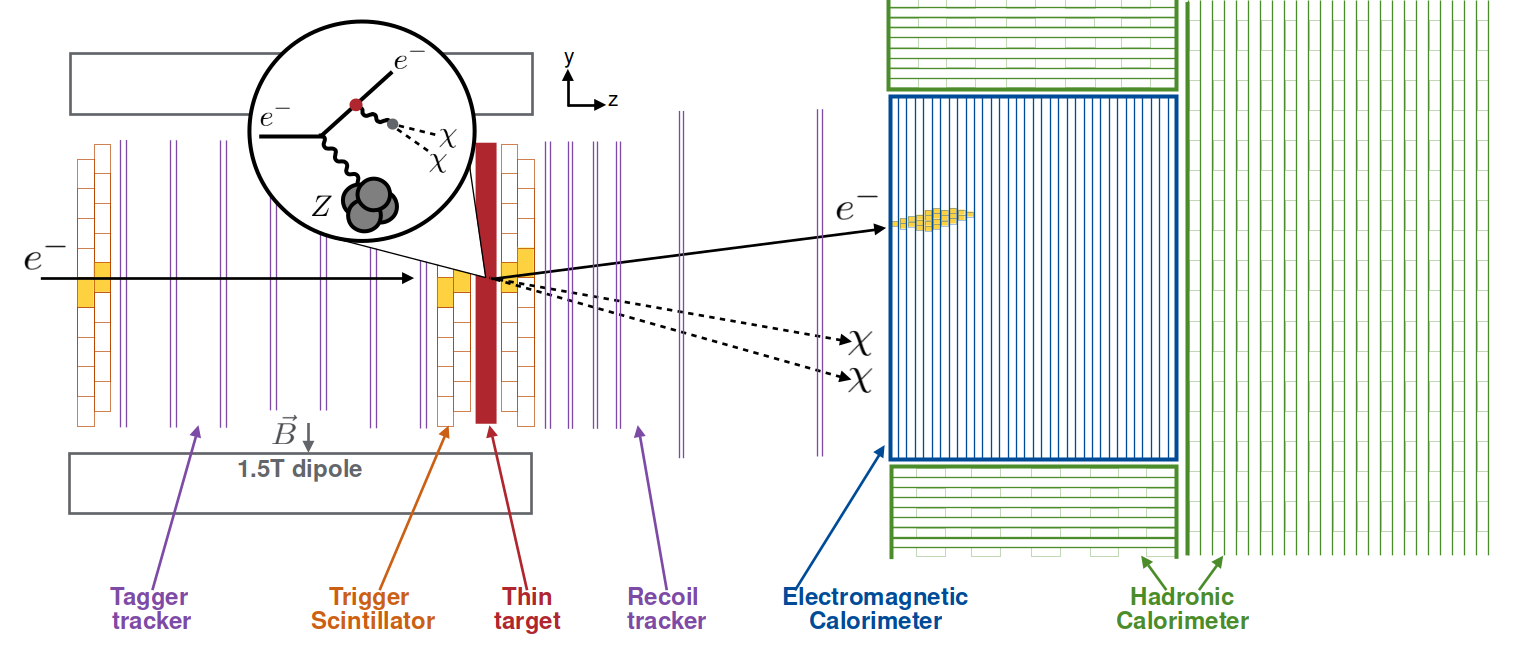
\includegraphics[width=\textwidth]{../figures/ldmx/experiment/detector.png}
      \\
      \resizebox{!}{\textwidth}{../figures/hps/experiment/hps-diagram}
    \end{column}
  \end{columns}
\end{frame}

\note[itemize]{
\item Background to get us on the same footing and using the same vocabulary
\item Motivate category of DM that experiments are searching for
\item Go through my analyses within both experiments
}

\ssection{Background}

\subsection{HEP Vocabulary}

\begin{frame}{Standard Model}
  \begin{columns}
    \begin{column}{0.4\textwidth}
      \begin{figure}
        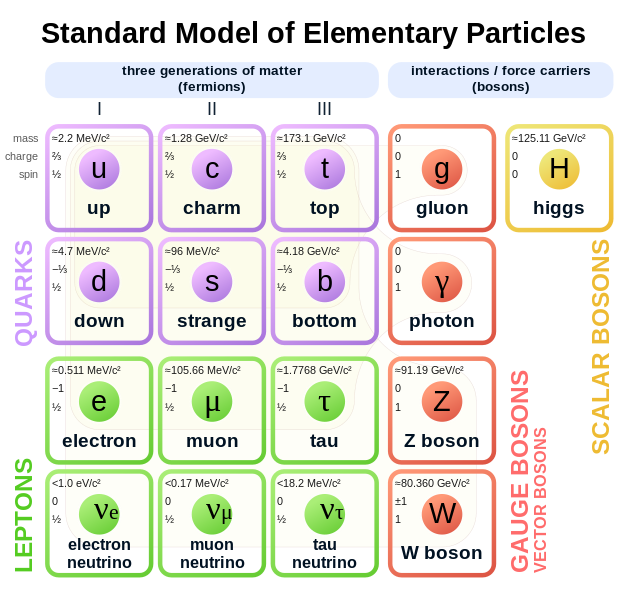
\includegraphics[width=\textwidth]{../figures/intro/Standard_Model_of_Elementary_Particles.svg.png}
        \caption{Credit to user Cush on wikipedia for providing this diagram.}
      \end{figure}
    \end{column}
    \begin{column}{0.6\textwidth}
      \begin{itemize}
        \item \boldcol{UMNSunny}{Law} -- summary of a set of consistent observations about phenomena
        \item \boldcol{UMNSunny}{Model} -- package of ``laws'' and their mathematical forms from which we can make predictions about future observations
        \item \boldcol{UMNSunny}{Orthogonal} -- used to emphasize that two different analyses are statistically independent
%        \item \boldcol{UMNSunny}{Event} -- a piece of data (one ``row'' of our data ``table''), a short period of time around a single electron entering the detector volume
      \end{itemize}
    \end{column}
  \end{columns}
\end{frame}

\note[itemize]{
\item Laws are summaries of observations and models
  are just packaging these laws with some mathematical sugar
\item The SM is the most quantitatively accurate physics model ever known to human kind.
\item It is a package of particles and their interactions (also represented by particles)
  from which we can -- with a specific mathematical framework -- make predictions about
  our observations.
\item \textbf{BUT} it fails to account for all observed phenomena (e.g. \emph{gravity})
}

%\begin{frame}{Feynman Diagram}
%\end{frame}
%
%\begin{frame}{Particle Mixing}
%  \begin{columns}
%    \begin{column}{0.4\textwidth}
%      \begin{figure}
%        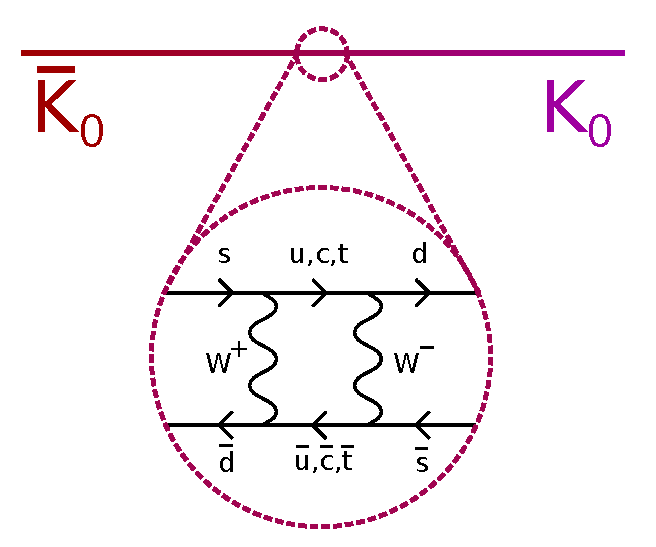
\includegraphics[width=\textwidth]{%
%          ../figures/intro/Kaon-box-diagram-with-bar.pdf%
%        }
%        \caption{Figure created by user NikNaks on Wikipedia.}
%      \end{figure}
%    \end{column}
%  \end{columns}
%\end{frame}
%
%\begin{frame}{Displaced Decay Vertices}
%  \begin{columns}
%    \begin{column}{0.5\textwidth}
%      \begin{figure}
%        \begin{tikzimage}[0.6\textwidth]{../figures/intro/bubble-chamber.jpeg}
%          \definecolor{brilliantrose}{rgb}{1.0, 0.33, 0.64}
%          % \draw[step=0.1,black,thin] (0.0,0.0) grid (1.0,1.0);
%          \node (prod) at (0.4,0.54) {};
%          \node[circle,draw=brilliantrose] (decay) at (0.515,0.54) {};
%          \draw[dashed,brilliantrose,thick] (prod) -- (decay);
%      
%          \node (beam1) at (0.1,0.5) {\color{brilliantrose}\(\pi^-\)};
%          \node (beam2) at (0.2,0.5) {};
%          \draw[->,brilliantrose,thick] (beam1) -- (beam2);
%        \end{tikzimage}
%        \caption{Image of CERN's first liquid hydrogen bubble chamber from 1960.}
%      \end{figure}
%    \end{column}
%  \end{columns}
%\end{frame}

\subsection{Dark Matter}
\begin{frame}{Dark Matter}
  \begin{columns}
    \begin{column}{0.5\textwidth}
      \begin{figure}
        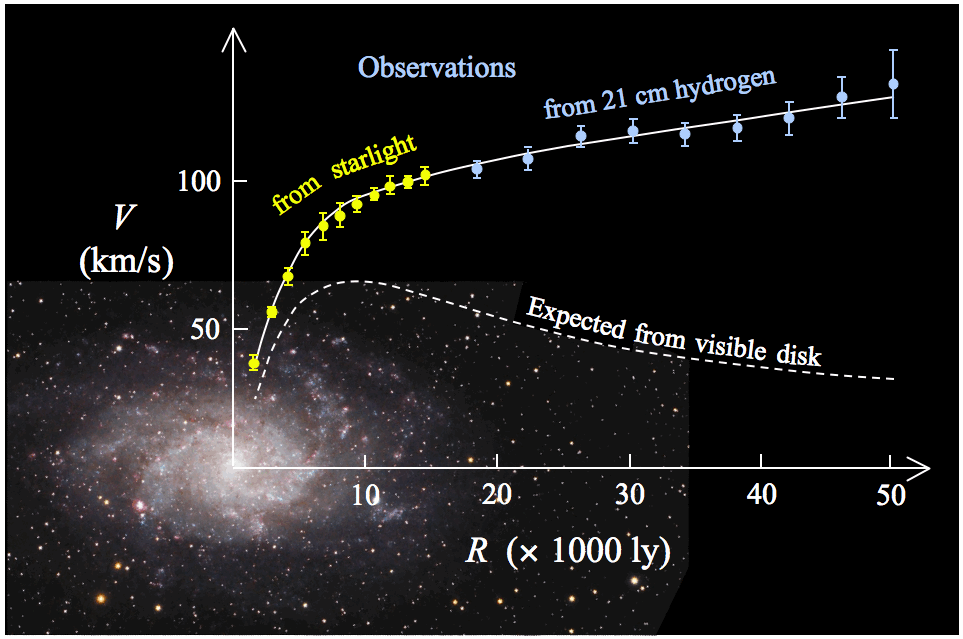
\includegraphics[width=\textwidth]{../figures/theory/rotation-curve-evidence-for-dm.png}
        \caption{Stuff is spinning too fast!}
      \end{figure}
    \end{column}
    \begin{column}{0.5\textwidth}
      \begin{figure}
        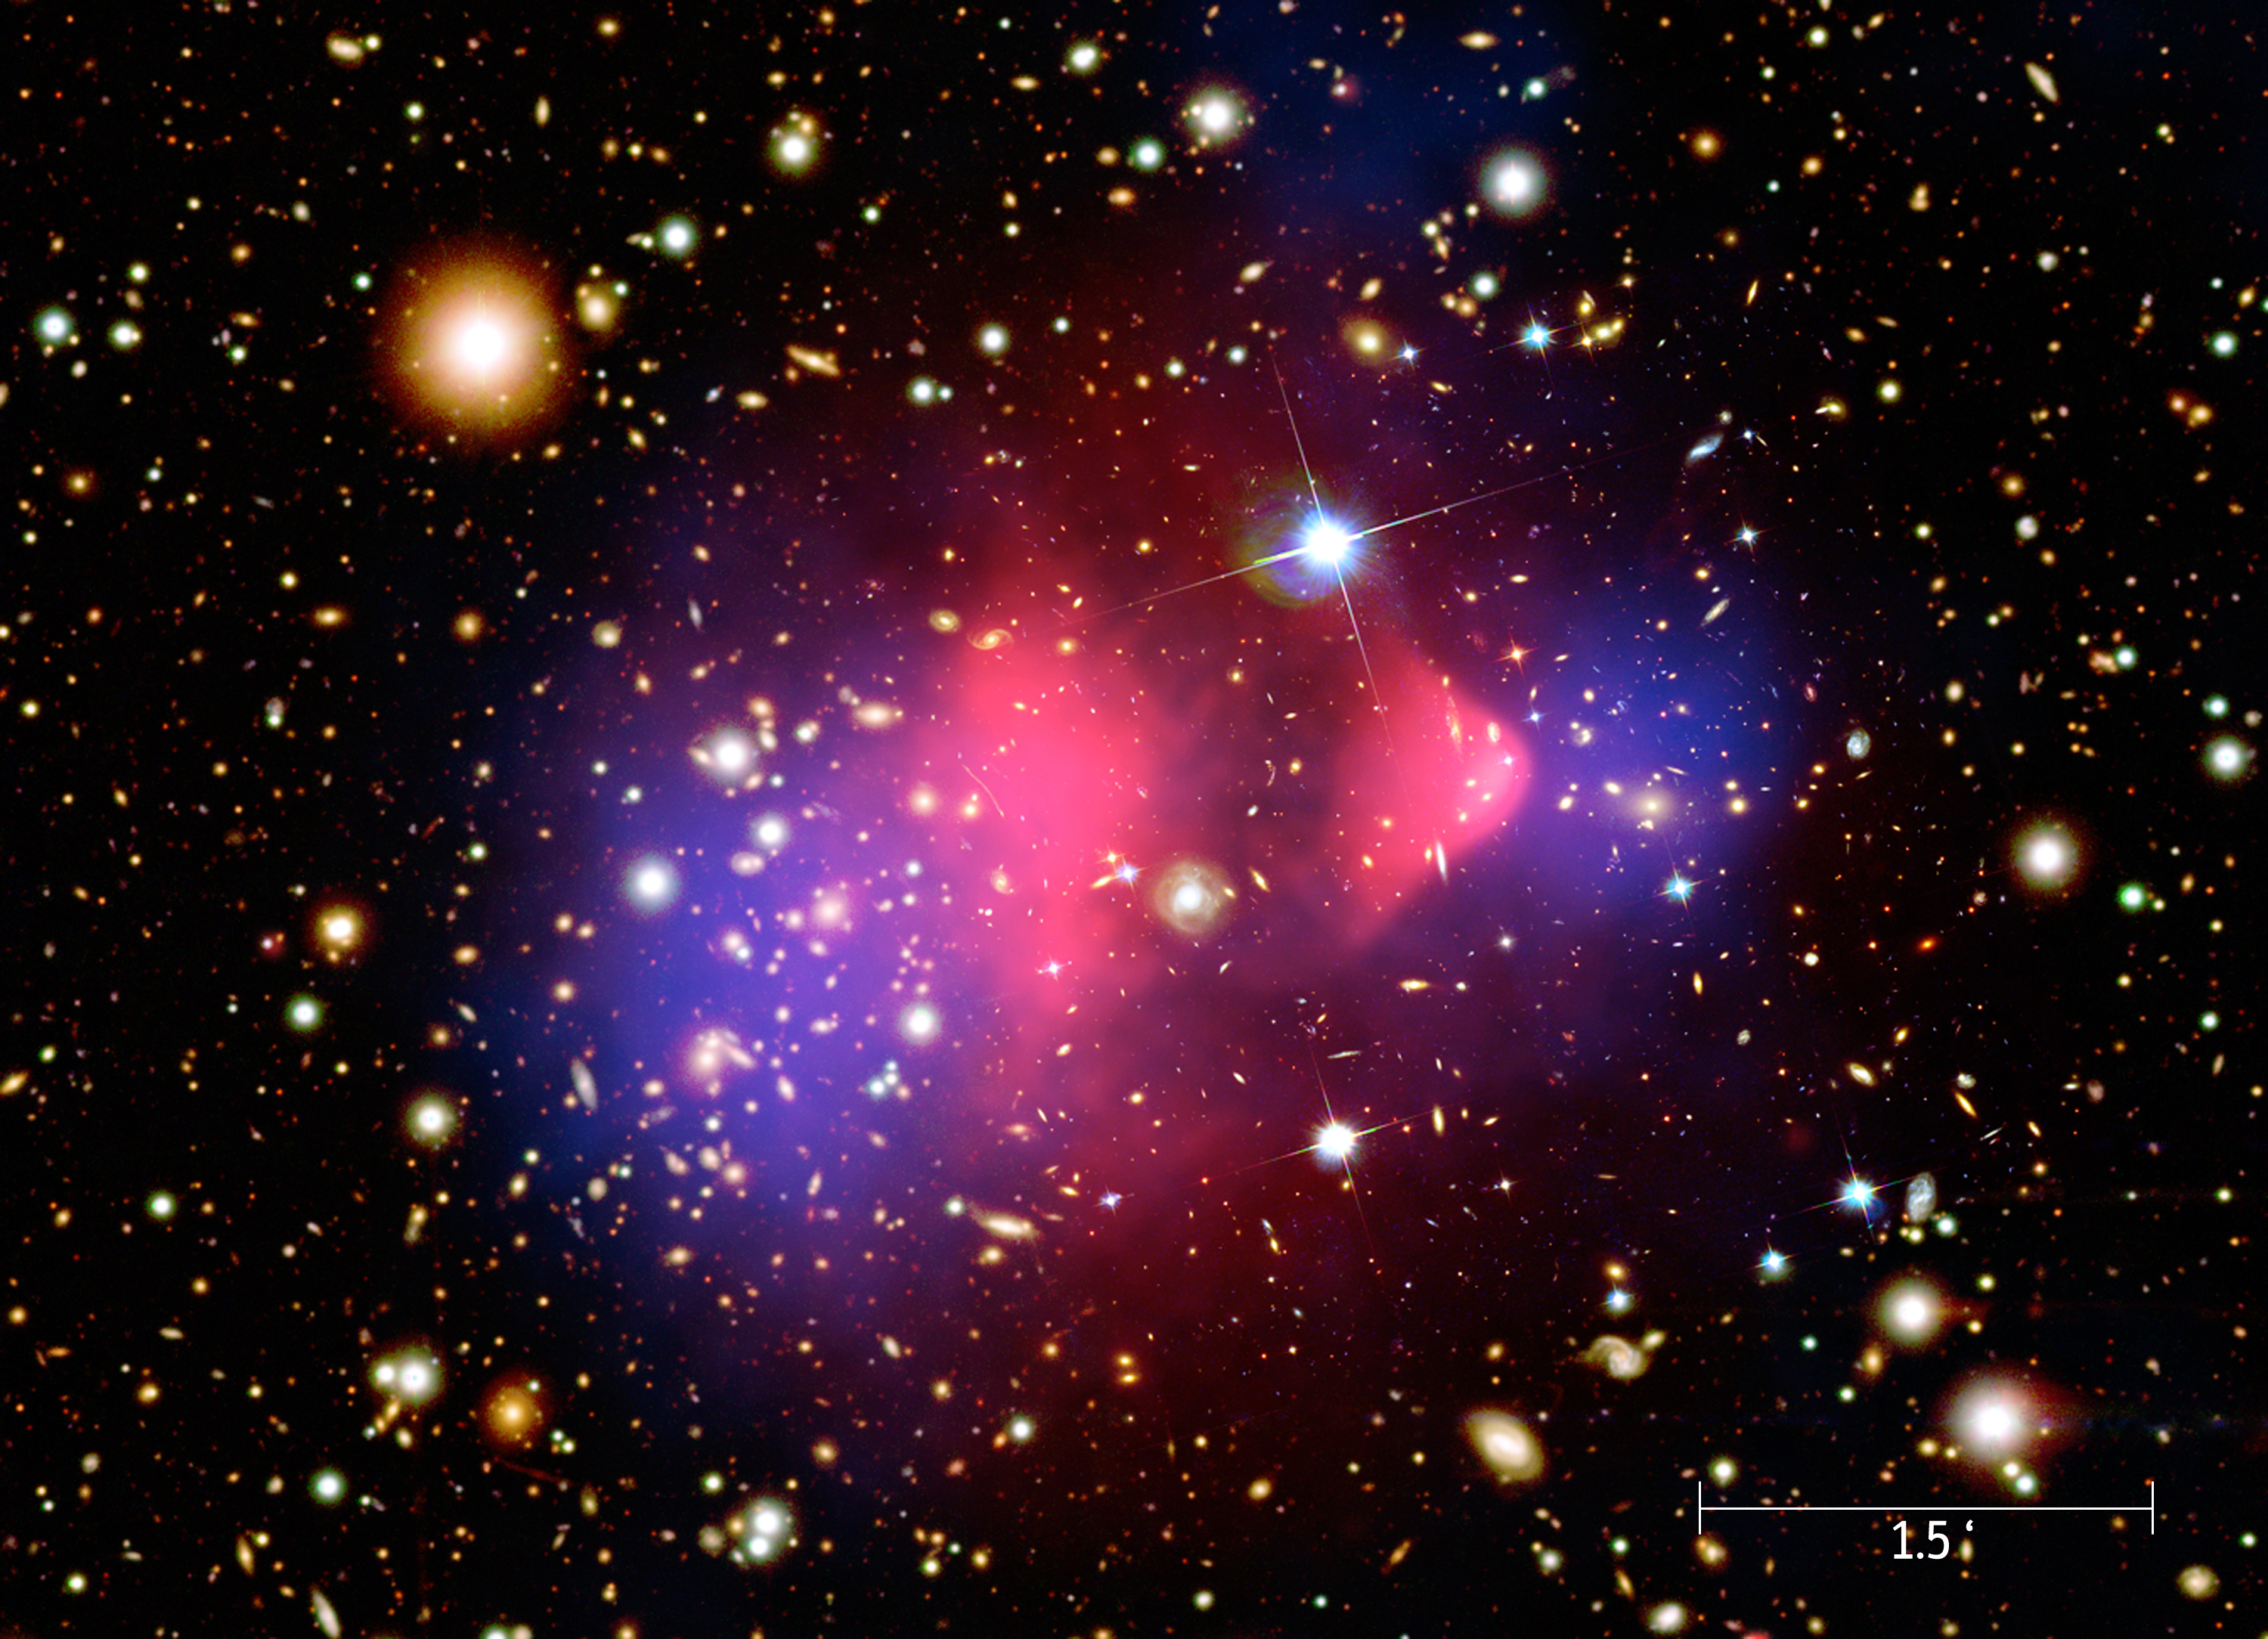
\includegraphics[width=\textwidth]{%
          ../figures/intro/bullet-cluster.jpg
        }
        \caption{Gravitational lensing (blue) and infrared (pink) observations
        show mass in different places!}
      \end{figure}
    \end{column}
  \end{columns}
\end{frame}

\note[itemize]{
\item One of the phenomena the SM doesn't account for is DM
\item We know it exists
\item Galactic rotation curves
  \begin{itemize}
    \item Expected from visible matter in dashed line
    \item Observed yellow/blue data points
    \item Either more matter we can't see helping hold these stars
      in or our model of gravity is wrong
  \end{itemize}
\item Grav lensing
  \begin{itemize}
    \item Very confident our model of gravity is correct from other measurements
    \item Additionally, grav lensing data of the bullet cluster
    \item Infrared signals (pink) differ in location than grav lensing (blue)
    \item ``heavy'' matter separate from ``visible'' matter
  \end{itemize}
}

\begin{frame}{Thermal Relic Dark Matter}
  \begin{block}{Narrow Wealth of Possibilities}
    Make the simple assumption that \ac{dm} has always been here.
  \end{block}
  \vfill
  \begin{figure}
    \centering
    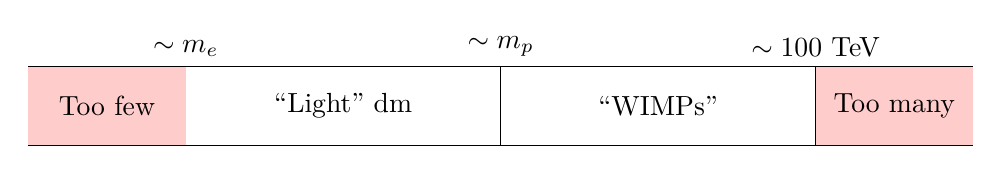
\begin{tikzpicture}
    % horizontal top/bottom lines
    \draw (0,0) -- (12,0);
    \draw (0,1) -- (12,1);
    % dividing lines along with relevant scale markers
    \draw (2,0) -- (2,1) node[above] {$\sim m_e$};
    \draw (6,0) -- (6,1) node[above] {$\sim m_p$};
    \draw (10,0) -- (10,1) node[above] {$\sim100~$TeV};
    % fill non-thermal ranges with light red
    \fill [red!20!white] (0,0) rectangle (2,1);
    \fill [red!20!white] (10,0) rectangle (12,1);
    % labels offering descriptions of ranges inside the boxes
    \node at (1,0.5) {Too few};
    \node at (4,0.5) {``Light'' \gls{dm}};
    \node at (8,0.5) {``WIMPs''};
    \node at (11,0.5) {Too many};
\end{tikzpicture}
    \caption{Mass scale of Thermal Relic \ac{dm}.
      The regions in red are excluded by applying the thermal relic assumption
      to our observations of the universe's early evolution.}
    \label{fig:dm-mass-scale}
  \end{figure}
  \boldcol{UMNSunny}{Both LDMX and HPS are searching for production of Light DM with electrons.}
\end{frame}

\note[itemize]{
\item Simplifying assumption: Dark Matter has always been here (like standard matter)
  and was in thermal equilibrium with standard matter in the early universe
\item (Observations of the CMB also imply this so its a decently motivated assumption.)
\item Limits the scale of mass of DM particles by connecting the mass to the interaction
  strength
\item Above $m_p\sim\qty{1}{\GeV}$, the interaction could be provided by the standard Weak
  force (so-called WIMPs), many experiments searching in this region
\item Below $m_p$, the interaction needs to be even weaker than the standard Weak force
\item Particles are lighter than WIMPs so referred to as Light DM
}

\begin{frame}{A Benchmark Model}
  \begin{columns}
    \begin{column}{0.5\textwidth}
      \begin{figure}
        \centering
        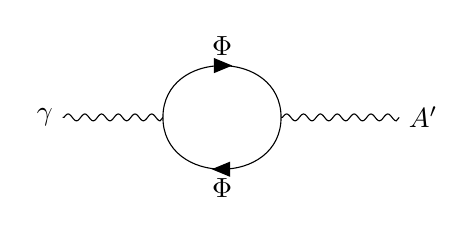
\begin{tikzpicture}
  \begin{feynman}
    \vertex (standard) {\(\gamma\)};
    \vertex [right=of standard] (loopleft);
    \vertex [right=of loopleft] (loopright);
    \vertex [right=of loopright] (dark) {\(A'\)};

    \diagram*{
    (standard)
    -- [photon] (loopleft)
    -- [fermion, half left, edge label=\(\Phi\)] (loopright)
    -- [photon] (dark),
    (loopright)
    -- [fermion, half left, edge label=\(\Phi\)] (loopleft),
    };
  \end{feynman}
\end{tikzpicture}

        \caption{Heavy field $\Phi$ enabling mixing between standard and dark photons.}
      \end{figure}

      The required connection between standard and dark sector provides an
      effective mixing of the standard and dark photons at our energy scales.
    \end{column}
    \begin{column}{0.5\textwidth}
      \begin{figure}
        \centering
        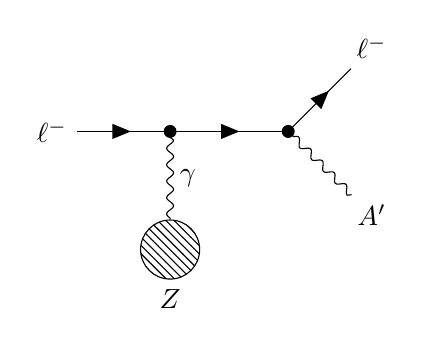
\begin{tikzpicture}
  \begin{feynman}
    \vertex (in) {\(\ell^-\)};
    \vertex [right=of in, dot] (nuc) {};
    \vertex [below=of nuc, blob, label={below:\(Z\)}] (nucleus) {};
    \vertex [right=of nuc, dot] (emit) {};
    \vertex [above right=of emit] (recoil) {\(\ell^-\)};
    \vertex [below right=of emit] (decay) {\(A'\)};
    % \vertex [above right=of decay] (chi2) {\(\overline{\chi}\)};
    % \vertex [below right=of decay] (chi1) {\(\chi\)};

    \diagram*{
    (in) -- [fermion] (nuc) -- [fermion] (emit) -- [fermion] (recoil),
    (nucleus) -- [photon, edge label'=\(\gamma\)] (nuc),
    (emit) -- [photon] (decay),
    % (emit) -- [photon, edge label'=\(A'\)] (decay),
    % (chi2) -- [fermion] (decay) -- [fermion] (chi1),
    };
  \end{feynman}
\end{tikzpicture}

        \caption{Dark bremsstrahlung process.}
      \end{figure}
      
      Mixing allows for a new process producing dark particles

      \boldcol{UMNSunny}{Both HPS and LDMX search for this production mechanism}
    \end{column}
  \end{columns}
\end{frame}

\note[itemize]{
\item The thermal relic assumption combined with curiosity for the lower masses
  requires the introduction of a new field which is presumably much heavier
  (i.e. harder to produce and observe) than our current energies.
\item This required connection does provide an effictive mixing of the standard
  and dark photons (like how kaons can mix) at our energy scales
\item Allowing for this mixing then gives a new process that can produce
  dark particles in our experiments -- dark bremsstrahlung
\item Both HPS and LDMX search for dark brem; however, they have different
  tactics to look for it
}

\ssection{LDMX}

\note[itemize]{
\item First, let's talk about the experiment I started with
\item The Light Dark Matter eXperiment is a \textbf{Missing Momentum} search for
  the dark bremsstralung production of dark particles with an electron beam
\item i.e. We assume that the dark photon that is produced ``stays in'' the dark sector
  and the momentum it had is not observable by our detector
}

\subsection{Experiment}
\begin{frame}{Missing Momentum Search}
  \begin{columns}
    \begin{column}{0.25\textwidth}
      \begin{block}{To Do MM Search}
        \begin{itemize}
          \item Know fate of every single electron
          \item Need faithful ID of even very rare SM processes
        \end{itemize}
      \end{block}
    \end{column}
    \begin{column}{0.7\textwidth}
      \begin{figure}
        \centering
        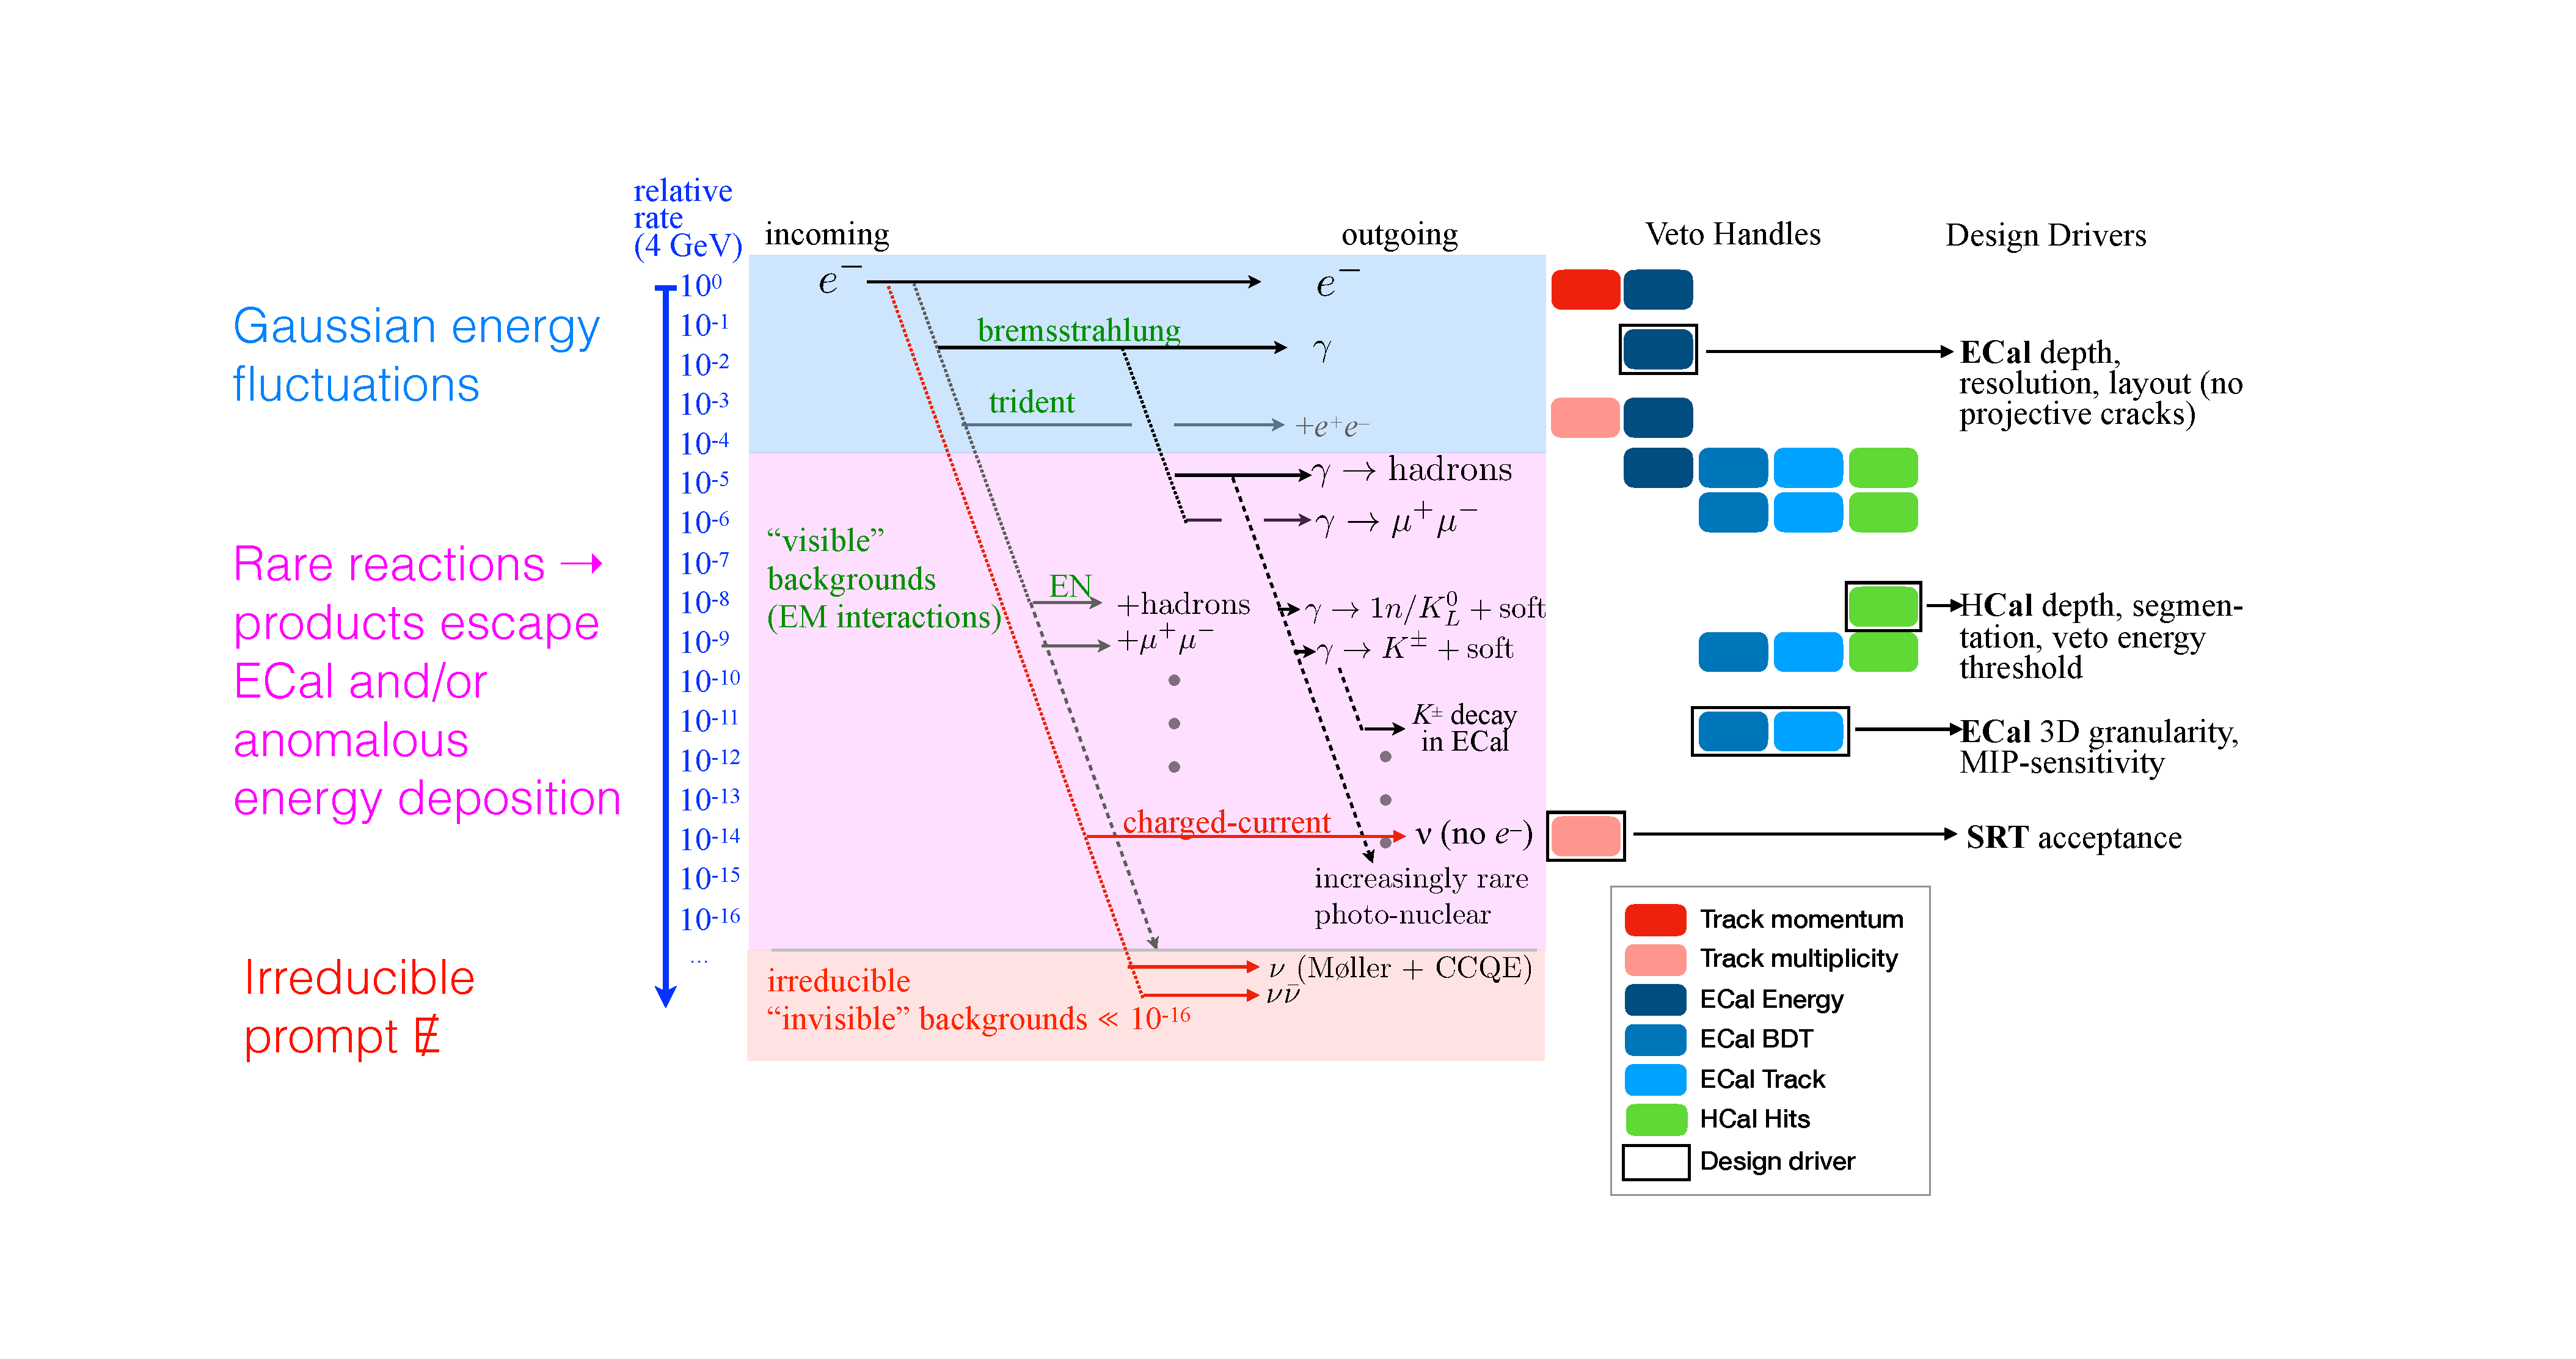
\includegraphics[width=\textwidth]{../figures/ldmx/experiment/reaction_staircase_with_designDrivers.pdf}
        \caption{Credit to Tim Nelson}
      \end{figure}
    \end{column}
  \end{columns}
\end{frame}

\note[itemize]{
\item LDMX, as mentioned, is a MM search and, to do MM, we need to
  know the fate of \textbf{every single electron}
  and be able to faithfully ID very rare SM processes
\item Here is a diagram of prominent SM processes ordered by their relative rate
\item Blue -- would happen in any target "brem" and "trident"
  \begin{itemize}
    \item Need tracker to measure incident and outgoing momenta of electron
    \item Need ECal to measure photon if brem ocurs
  \end{itemize}
\item Pink -- sometimes the photon gets up to some funky stuff in the ECal
  that makes the ECal's measurement more complicated
  \begin{itemize}
    \item rarer processes requiring more granular information about what happens
    \item stuff that is hard for the ECal to measure motivates a seconadary
      calorimeter for these particles (HCal)
  \end{itemize}
\item Red -- very rare processes that we will not be able to remove
  (but could constrain using measurements of these processes by other experiments)
}

\begin{frame}{Experiment}
  \begin{figure}
    \centering
    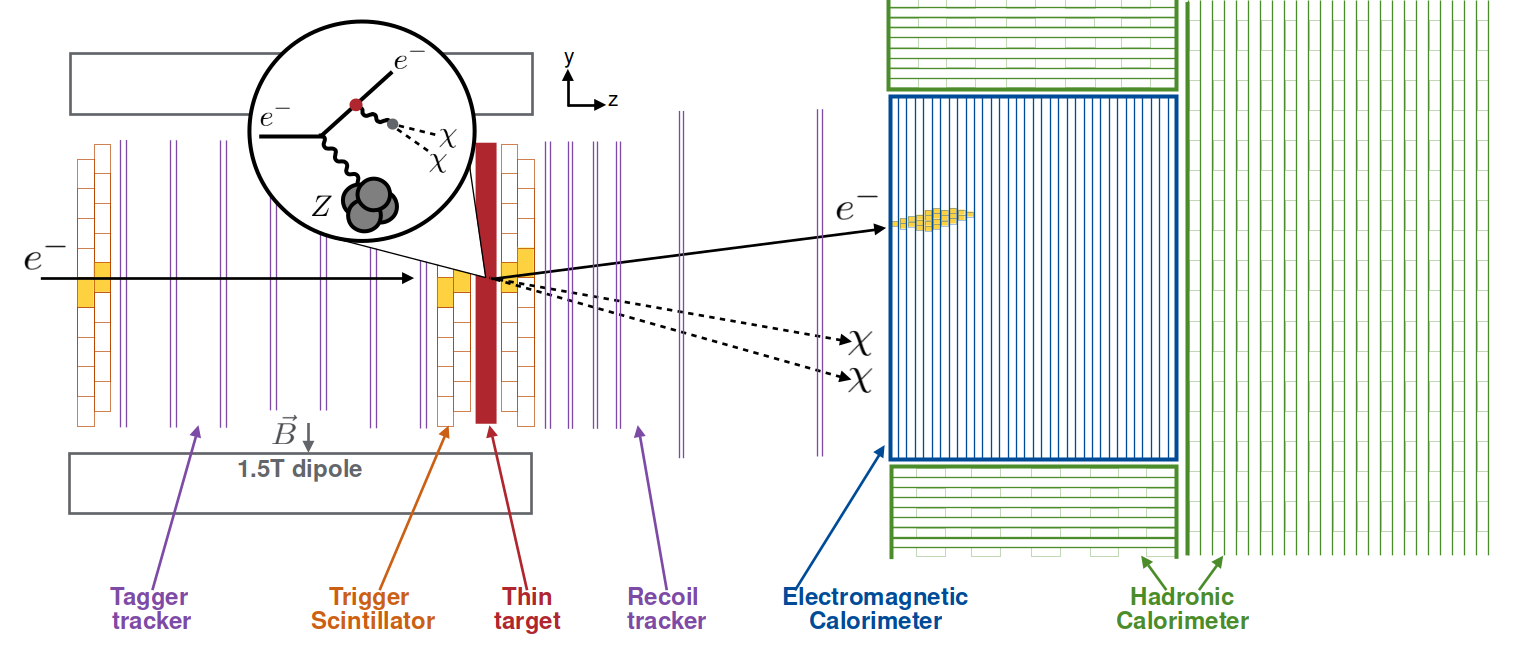
\includegraphics[width=\textwidth]{../figures/ldmx/experiment/detector.png}
    \caption{Credit to Christian Herwig for original diagram}
  \end{figure}
\end{frame}

\note[itemize]{
\item These processes motivate a staged design
  \begin{itemize}
    \item a tracker (tagger for incoming and recoil for outgoing)
    \item ECal for electrons/positrons and photons
    \item HCal for hadrons (e.g. protons/neutrons) and muons
    \item a TrigScint to quickly count electrons and help ECal make trigger decision in time.
  \end{itemize}
\item Hosted at SLAC Natl Accelerator Lab, recieving beam from LCLS-II 
\item Beam facility upgrading from \qty{4}{\GeV} to \qty{8}{\GeV}, LDMX may see
  some \qty{4}{\GeV} beam depending on how schedules line up but a majority
  of data will be taken with \qty{8}{\GeV}
\item \textbf{Thin target to help momentum resolution.} -- most electrons pass through
  only minimally interacting
\item Can we still use this data we would collect anyways?
}

\subsection{New, Orthogonal Analysis Channel}
\begin{frame}{Using the ECal as Target}
  \begin{figure}
    \centering
    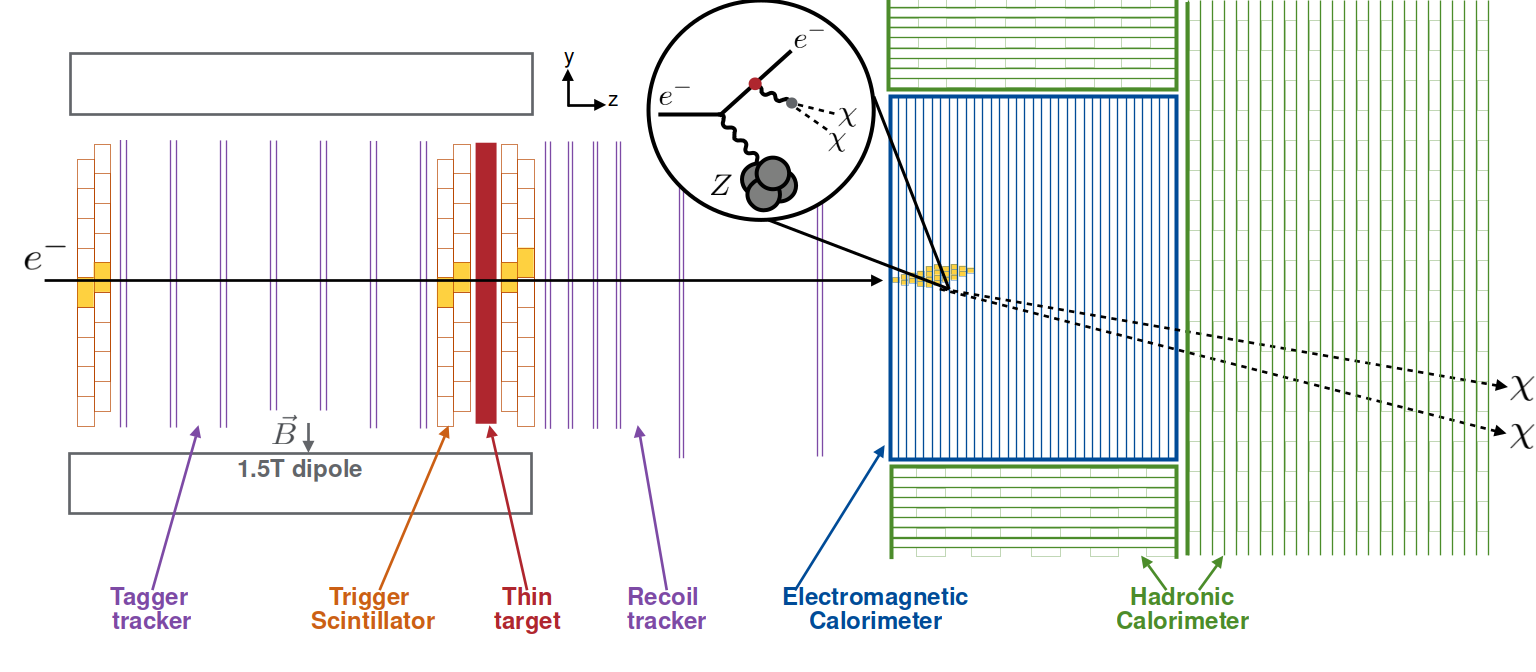
\includegraphics[width=\textwidth]{figs/detector-eat-signal.png}
    \caption{Credit to Christian Herwig for original diagram}
  \end{figure}
\end{frame}

\note[itemize]{
\item Yes we can!
\item If the dark brem process exists and would happen in the thin target,
  it would also happen within other parts of our detector -- namely the ECal
  which has a lot of material and would recieve similar numbers of electrons as
  the target
\item Use the Ecal as another Target for our dark brem search
\item Shift focus to \textbf{Missing Energy} search
\item Use upstream detectors to confirm near-beam-energy electron entering ECal \\
  (orthogonality condition, MM search requires significant loss within thin target)
\item ECal has more material $\to$ more ``chances'' for dark brem to happen \\
  (about $\sim 3$ times more when accounting for acceptance and trigger efficiency)
}

\begin{frame}{Familiar Culprits}
  \begin{columns}
    \begin{column}{0.45\textwidth}
      \begin{figure}
        \centering
        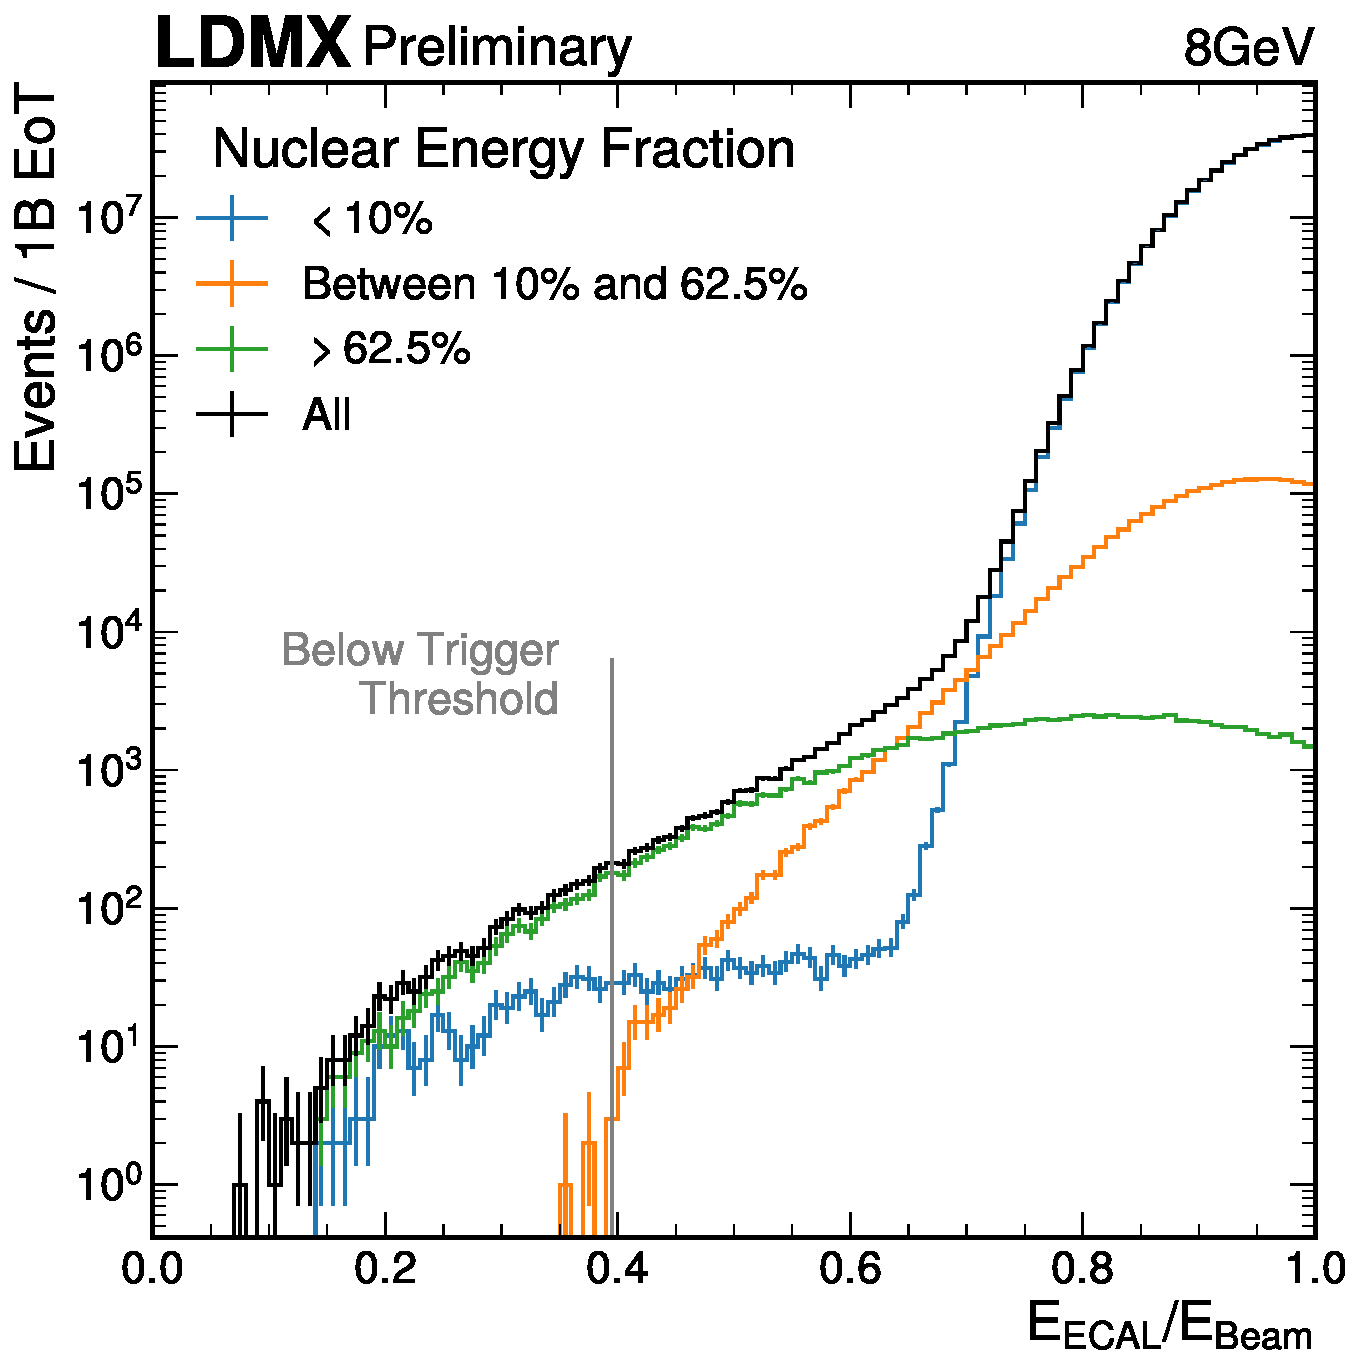
\includegraphics[width=0.9\textwidth]{../figures/ldmx/simulation/8gev-ecal-by-nuc.pdf}
        \caption{\footnotesize Reconstructed energy fraction separated by 
        energy going into nuclear processes.}
      \end{figure}
    \end{column}
    \begin{column}{0.55\textwidth}
      \begin{block}{Simulation Requirement}
        Electron reaches ECal with $> 87.5\%$ of the original beam energy.
      \end{block}

      Standard processes mimicking our signal are similar to thin-target analysis
      \begin{itemize}
        \item ``Nuclear'' processes (electrons and photons interacting with nuclei to produce hadrons)
        \item Muon pair production (via high-energy photon)
      \end{itemize}
    \end{column}
  \end{columns}
\end{frame}

\note[itemize]{
\item The standard processes we need to identify are familiar culprits
  \begin{itemize}
    \item ``Nuclear'' processes
    \item ``Di-Muon'' production via high-energy photons
  \end{itemize}
\item Handling these background will depend on the volume of data we collect
}

\subsection{Sensitivity in Early Running}
\begin{frame}{Target Data Volume}
  \begin{columns}
    \begin{column}{0.45\textwidth}
      \begin{figure}
        \centering
        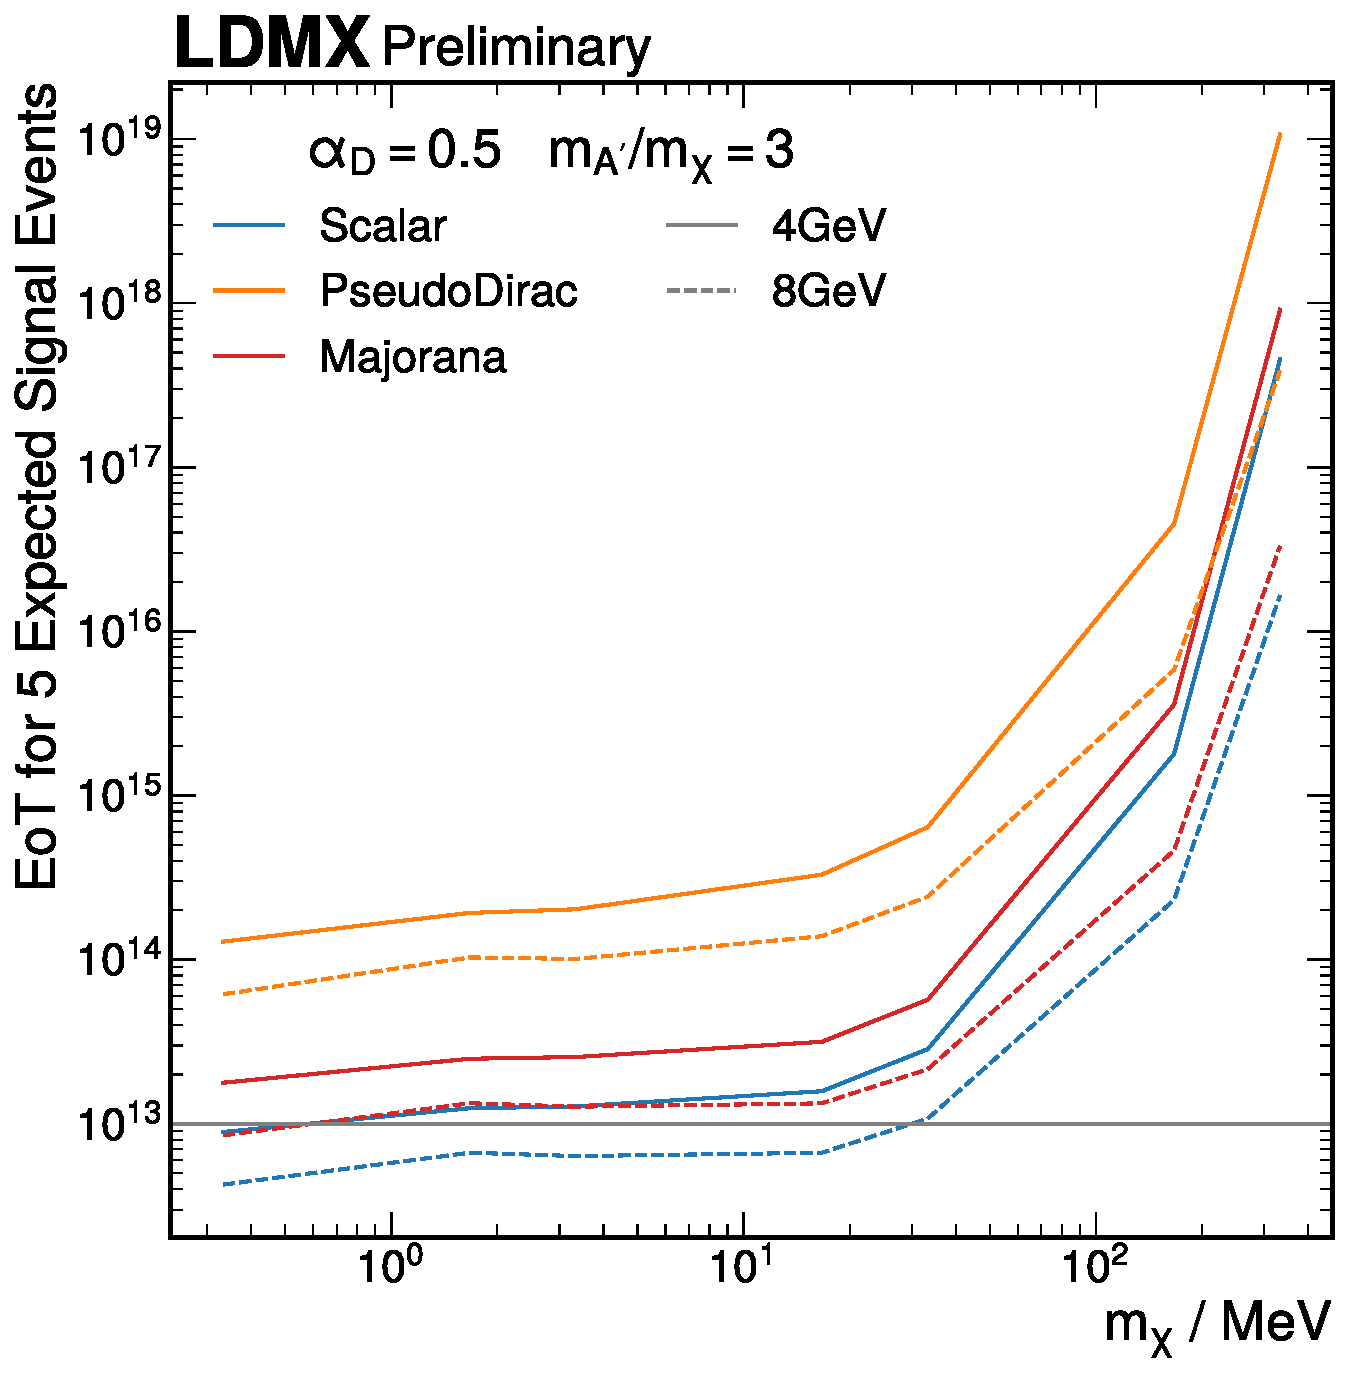
\includegraphics[width=0.9\textwidth]{figs/eot-for-n-signal.pdf}
      \end{figure}
    \end{column}
    \begin{column}{0.55\textwidth}
      \begin{itemize}
        \item Targeting $\sim 5$ expected signal events for a few possible thermal relic models
        \item Focus on \num{1e13} \ac{eot}
        \item $\sim\qty{2}{week}$ nominal beam time
      \end{itemize}

      \begin{block}{Early Running}
        Focus on first contact with real data
      \end{block}
    \end{column}
  \end{columns}
\end{frame}

\note[itemize]{
\item We choose to focuse on \num{1e13} \ac{eot} for two key reasons
  \begin{enumerate}
    \item Amounts to $\sim 5$ signal events for a few possible thermal relic models \\
      (discovery is hard for EaT -- focusing on exclusion)
    \item Only would require $\sim\qty{2}{week}$ nominal beam time
  \end{enumerate}
\item Also points out that this EaT analysis can probably be a first-contact analysis
\item Add goals of simplicity and robustness to insulate analysis from complexities of first data
}

\begin{frame}{Mid-shower Simulation Samples}
  Requirements
  \begin{itemize}
    \item Save computer time
    \item Save computer space
    \item focus on specific processes that are interesting to us \\
      (signal itself or standard processes that mimick it)
  \end{itemize}
  \vfill
  \begin{block}{Solution for Mid-Shower Samples}
    \begin{enumerate}
      \item \boldcol{UMNSunny}{Sort} simulation so higher-energy particles go first
      \item \boldcol{UMNSunny}{Bias} the process-of-interest for these high-energy particles
      \item \boldcol{UMNSunny}{Filter} out events that do not pass criteria
    \end{enumerate}
  \end{block}
\end{frame}

\note[itemize]{
\item Don't have real data yet -- need to simulate it
\item We also are focusing on specific processes (``Nuclear'' and ``Dimuon'') ocurring
  within the developing shower in the ECal
\item \textit{Requirements}
\item Developed a method to do just that -- \textit{Solution}
\item Since LDMX's beam provider LCLS-II is being upgraded separately,
  we have the potential to observe \fourgev or \eightgev beams.
\item With this technique, generated ``Nuclear'' and ``Dimuon'' samples
  statistically equivalent to \num{1e13} \ac{eot} -- combined to represent
  total ``Background''
\item \eightgev is more likely so I'll default to those figures
}

\begin{frame}{Missing Energy Signature}
  \begin{columns}
    \begin{column}{0.5\textwidth}
      \begin{enumerate}
        \item Energy measurement significantly below beam energy
        \item Nothing ``escaped'' the ECal
        \item Nothing ``funky'' happened in the ECal
      \end{enumerate}
    \end{column}
    \begin{column}{0.5\textwidth}
      \color{red}TODO: diagrams of escaping and funky
    \end{column}
  \end{columns}
\end{frame}

\note[itemize]{
\item Three key ingredients for our missing energy search
}

\begin{frame}[t]{Cuts for Missing Energy Signature}
  \begin{columns}[t]
    \begin{column}{0.32\textwidth}
      \centering
      \framesection{Low Energy Measurement}
      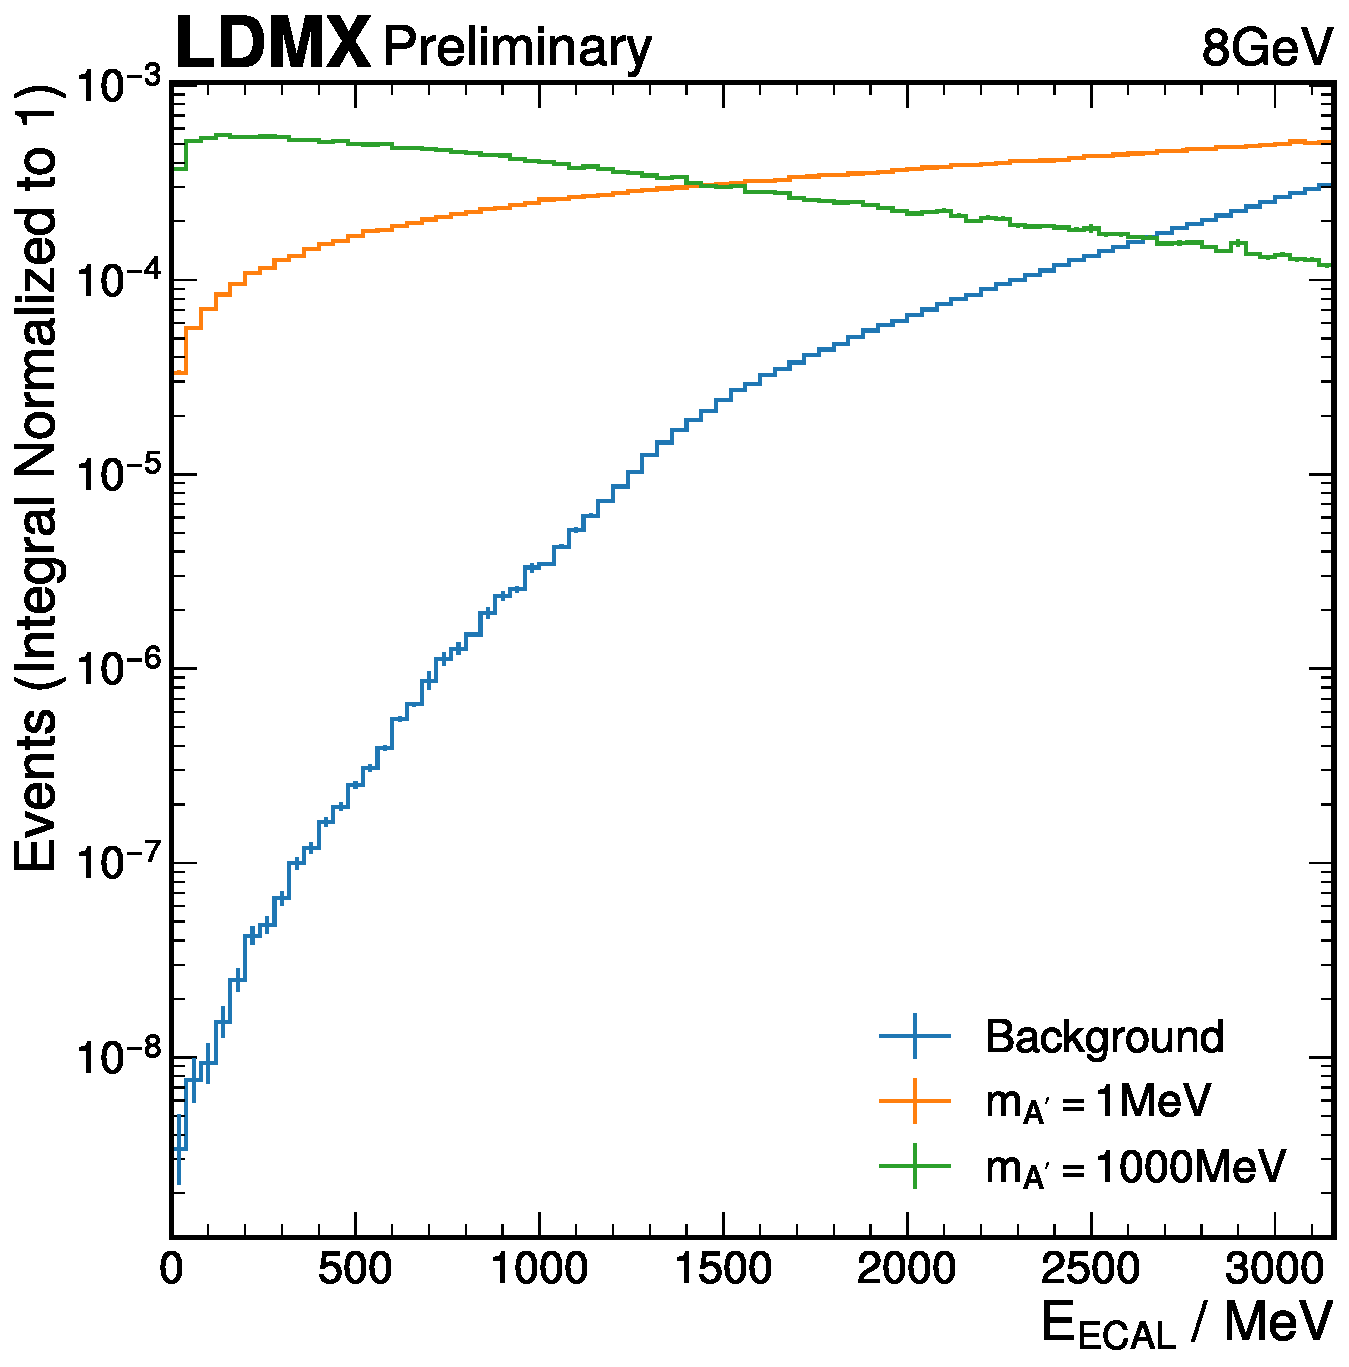
\includegraphics[width=0.9\textwidth]{../figures/ldmx/analysis/energy-after-trigger-8gev.pdf}
      {
        \footnotesize
        \begin{itemize}
          \item Use ME trigger same as nominal analysis
          \item Require lower energy on sum over all layers
        \end{itemize}
      }
    \end{column}
    \begin{column}{0.32\textwidth}
      \centering
      \framesection{Nothing Escapes}
      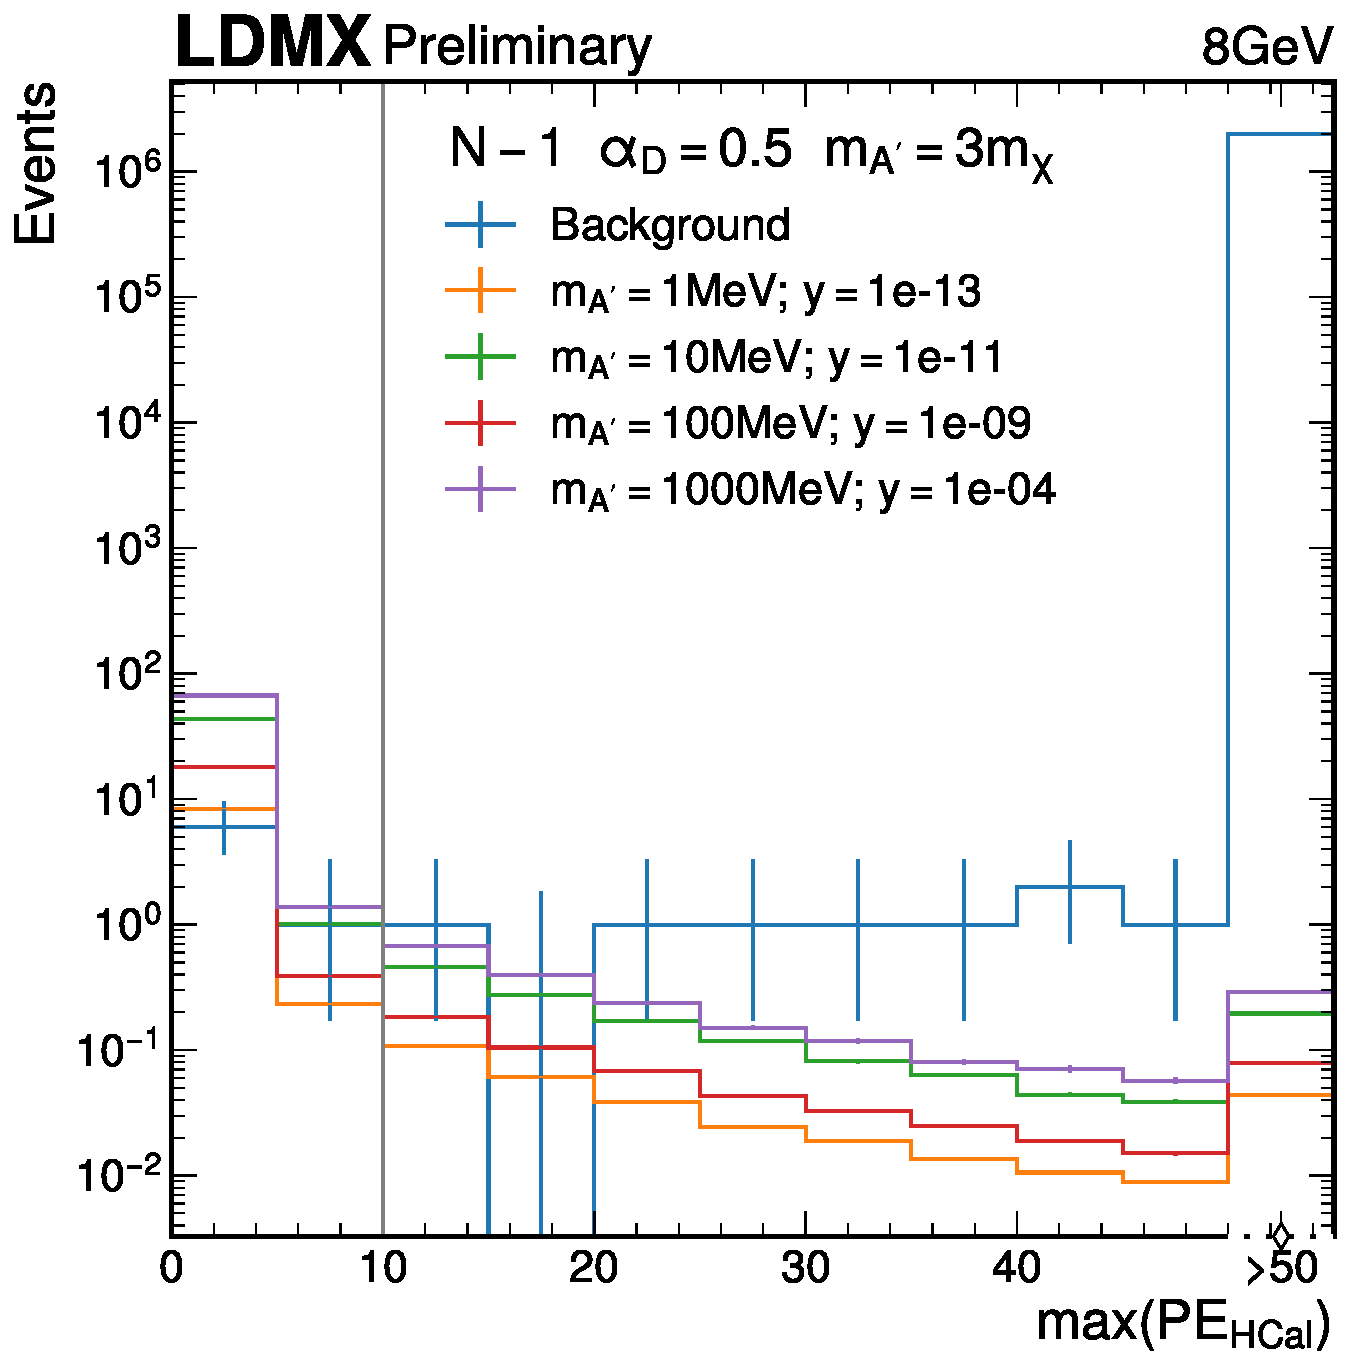
\includegraphics[width=0.9\textwidth]{../figures/ldmx/analysis/nm1-hcal-max-pe-8gev-1e13norm.pdf}
      {
        \footnotesize
        No bar within the HCal with a total signal $> \qty{10}{PE}$
      }
    \end{column}
    \begin{column}{0.32\textwidth}
      \centering
      \framesection{Nothing Funky}
      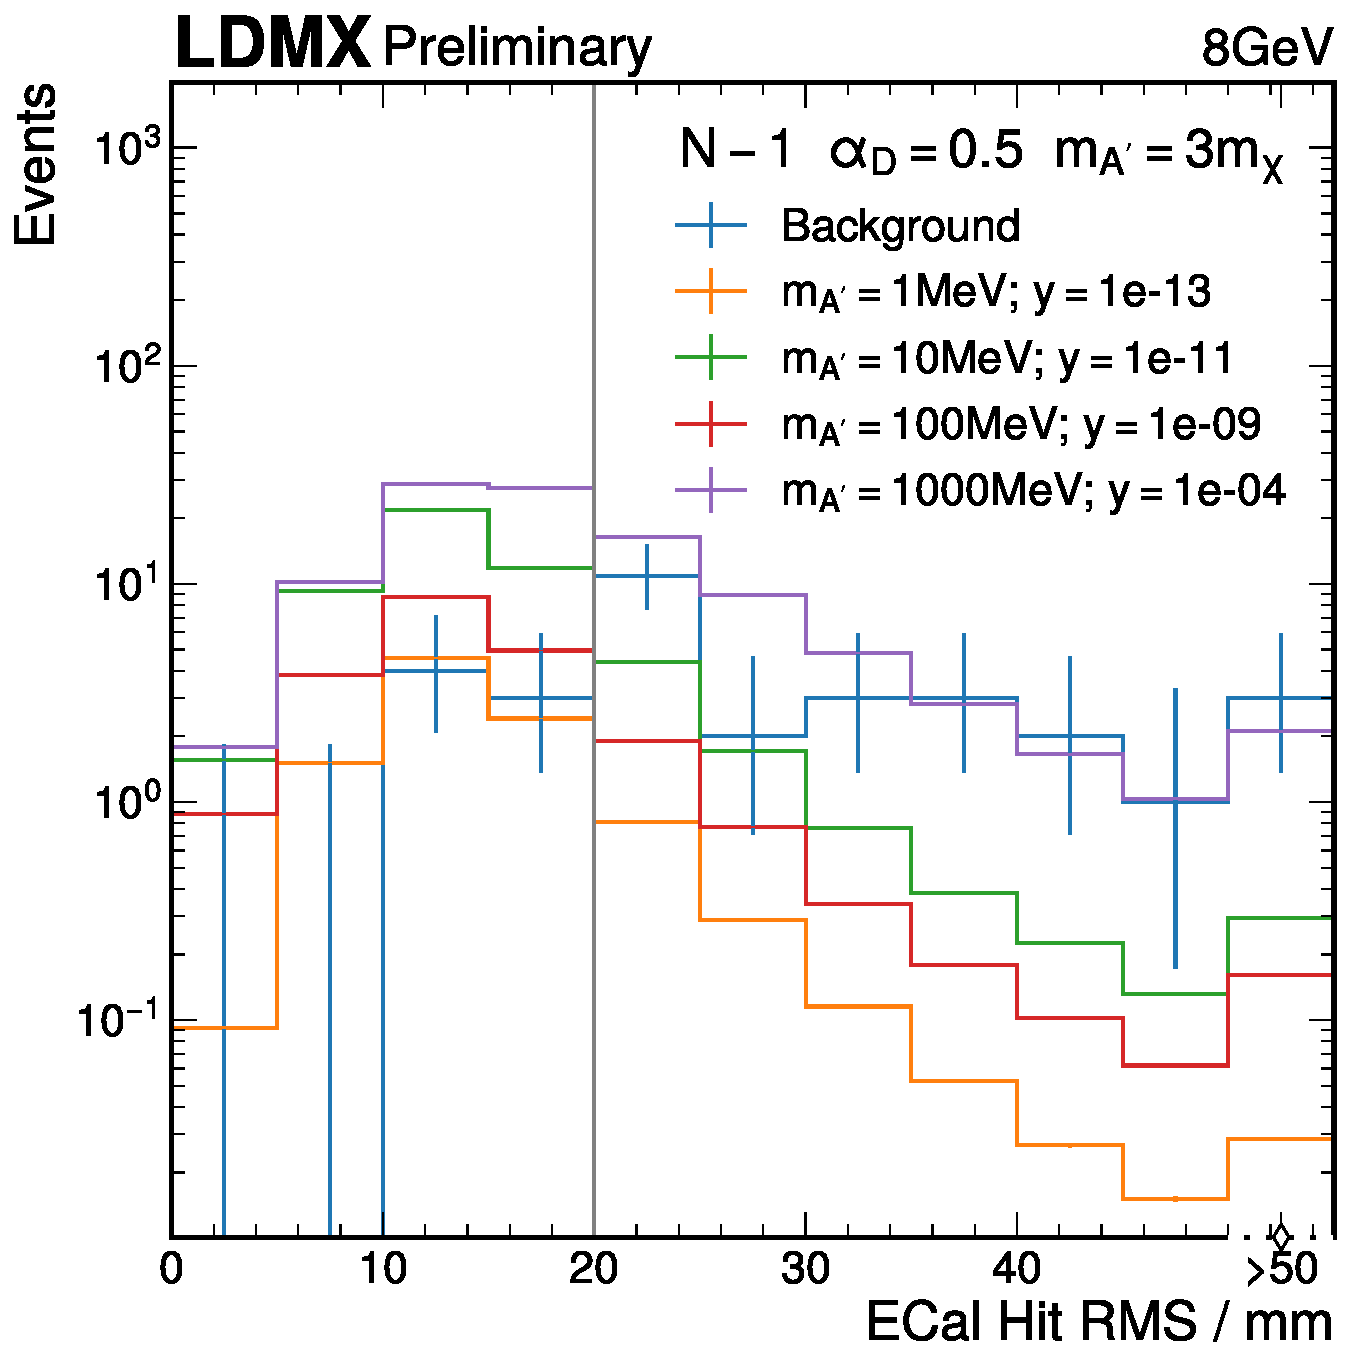
\includegraphics[width=0.9\textwidth]{../figures/ldmx/analysis/nm1-ecal-rms-8gev-1e13norm.pdf}
      {
        \footnotesize
        Energy-weighted transverse RMS of hits with amplitude $\geq 0.5E_\mathrm{MIP}$
        to be $<\qty{20}{\mm}$
      }
    \end{column}
  \end{columns}
\end{frame}

\note[itemize]{
\item Accomplish this signature using three specific variables
\item Energy sum
  \begin{itemize}
    \item After using the same trigger as the thin target MM analysis
    \item Sum over all layers and require the measurement to be \qty{400}{\MeV} less
      than the threshold used for the trigger
    \item Helps avoid contamination from miscalibrations in early running
  \end{itemize}
\item \textit{Explanatory Comma} N-1 plots show the cut variable in question after
  all other selections have been applied. Evidence that the cut is being helpful.
\item Quiet HCal
  \begin{itemize}
    \item Typical signals from muons are $\sim\qty{80}{PE}$ and other particles have higher typical signals
    \item Require no bar within HCal to register signal higher than \qty{10}{PE}
  \end{itemize}
\item Thin Shower
  \begin{itemize}
    \item Indirectly remove ``funky'' interactions by requiring hits to be close to each other
    \item Avoid hits below half a MIP 
  \end{itemize}
}

\begin{frame}{Summary of Cutflow}
  \begin{table}
    \begin{tabular}{|r|c||c|c|c|c|}
    \hline
    \multirow{2}{*}{Analysis Stage for \fourgev Beam} & 
      Background & 
      \multicolumn{4}{c|}{Signal Efficiency (\%)} 
      \\ \cline{3-6} 
    & Event Yield & $1$~MeV & $10$~MeV & $100$~MeV & $1$~GeV \\ \hline
    \ecal Trigger ($E_{20} < 1.5$~GeV) &
      \num{4.60e+07} & 58 & 67 & 71 & 83 \\
    \ecal Energy ($E_{\mathrm{\ecal}} < 1.1$~GeV) & 
      \num{1.95e+06} & 35 & 48 & 53 & 72 \\
    $\max(\text{PE}_{\text{\hcal}}) < 10$ &
      \num{1.15e+03} & 34 & 47 & 52 & 69 \\
    ECal Hit RMS $< 20\;\mathrm{mm}$ &
      126 & 28 & 37 & 41 & 33 \\
    \hline
    \hline
    \multirow{2}{*}{Analysis Stage for \eightgev Beam} & 
      Background & 
      \multicolumn{4}{c|}{Signal Efficiency (\%)} 
      \\ \cline{3-6} 
    & Event Yield & $1$~MeV & $10$~MeV & $100$~MeV & $1$~GeV \\ \hline
    \ecal Trigger ($E_{20} < 3.16$~GeV) &
      \num{6.10e+07} & 66 & 74 & 79 & 89 \\
    \ecal Energy ($E_{\text{\ecal}} < 2.76$~GeV) &
      \num{6.88e+06} & 52 & 63 & 69 & 84 \\
    $\max(\text{PE}_{\text{\hcal}}) < 10$ &
      31.8 & 50 & 61 & 67 & 81 \\
    ECal Hit RMS $< 20\;\mathrm{mm}$ &
      7 & 43 & 52 & 56 & 52
    \\ \hline
\end{tabular}

    \caption{Cutflow for this analysis.
    Background event yields are estimates for $10^{13}$ EoT.}
  \end{table}
  \vfill
\end{frame}

\note[itemize]{
\item After these simple, physically-defined selections -- background is reduced by 5 or 7
  orders of magnitude while maintaining $\sim\qty{50}{\%}$ signal efficiency
\item Still some background left, how to handle it?
}

\begin{frame}{Multi-Channel Analysis}
  \begin{block}{}
    Search within adjacent ``channels'' or ``bins'' using different shapes to our advantage
  \end{block}
  \vfill
  \begin{columns}
    \begin{column}{0.35\textwidth}
      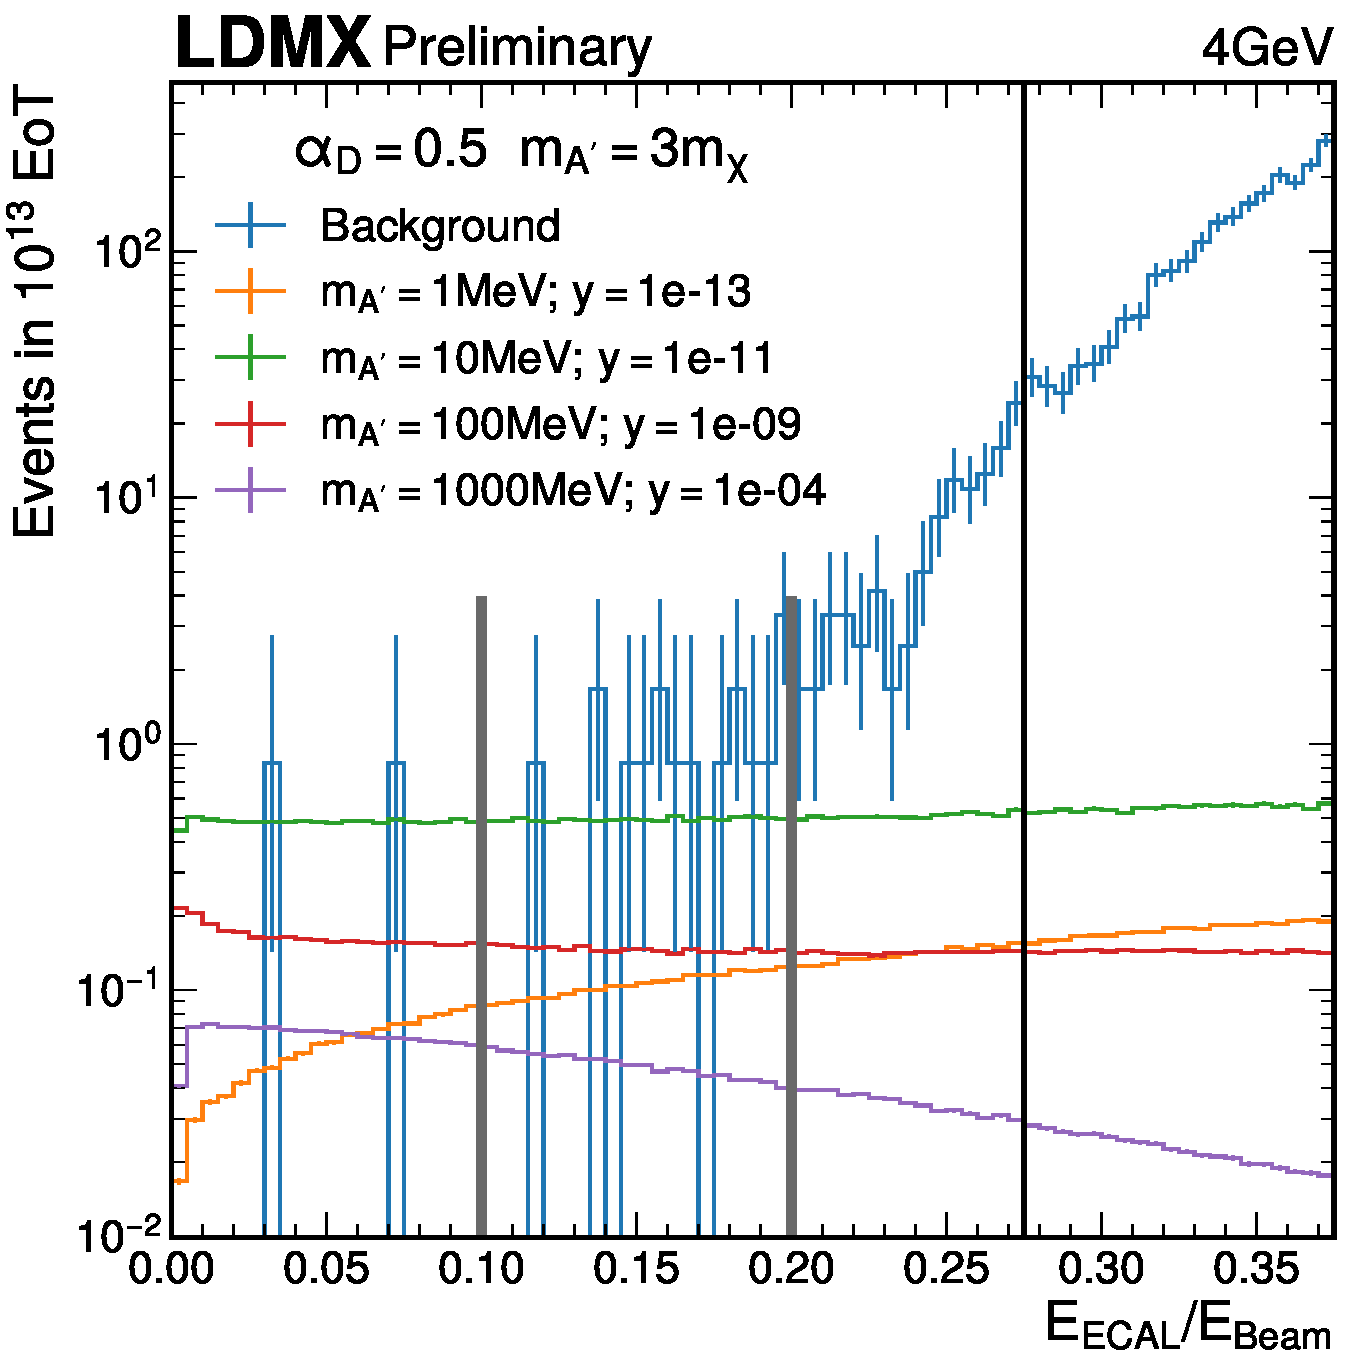
\includegraphics[width=\textwidth]{%
        ../figures/ldmx/analysis/final-selection-with-ana-bin-edges-4gev.pdf}
    \end{column}
    \begin{column}{0.35\textwidth}
      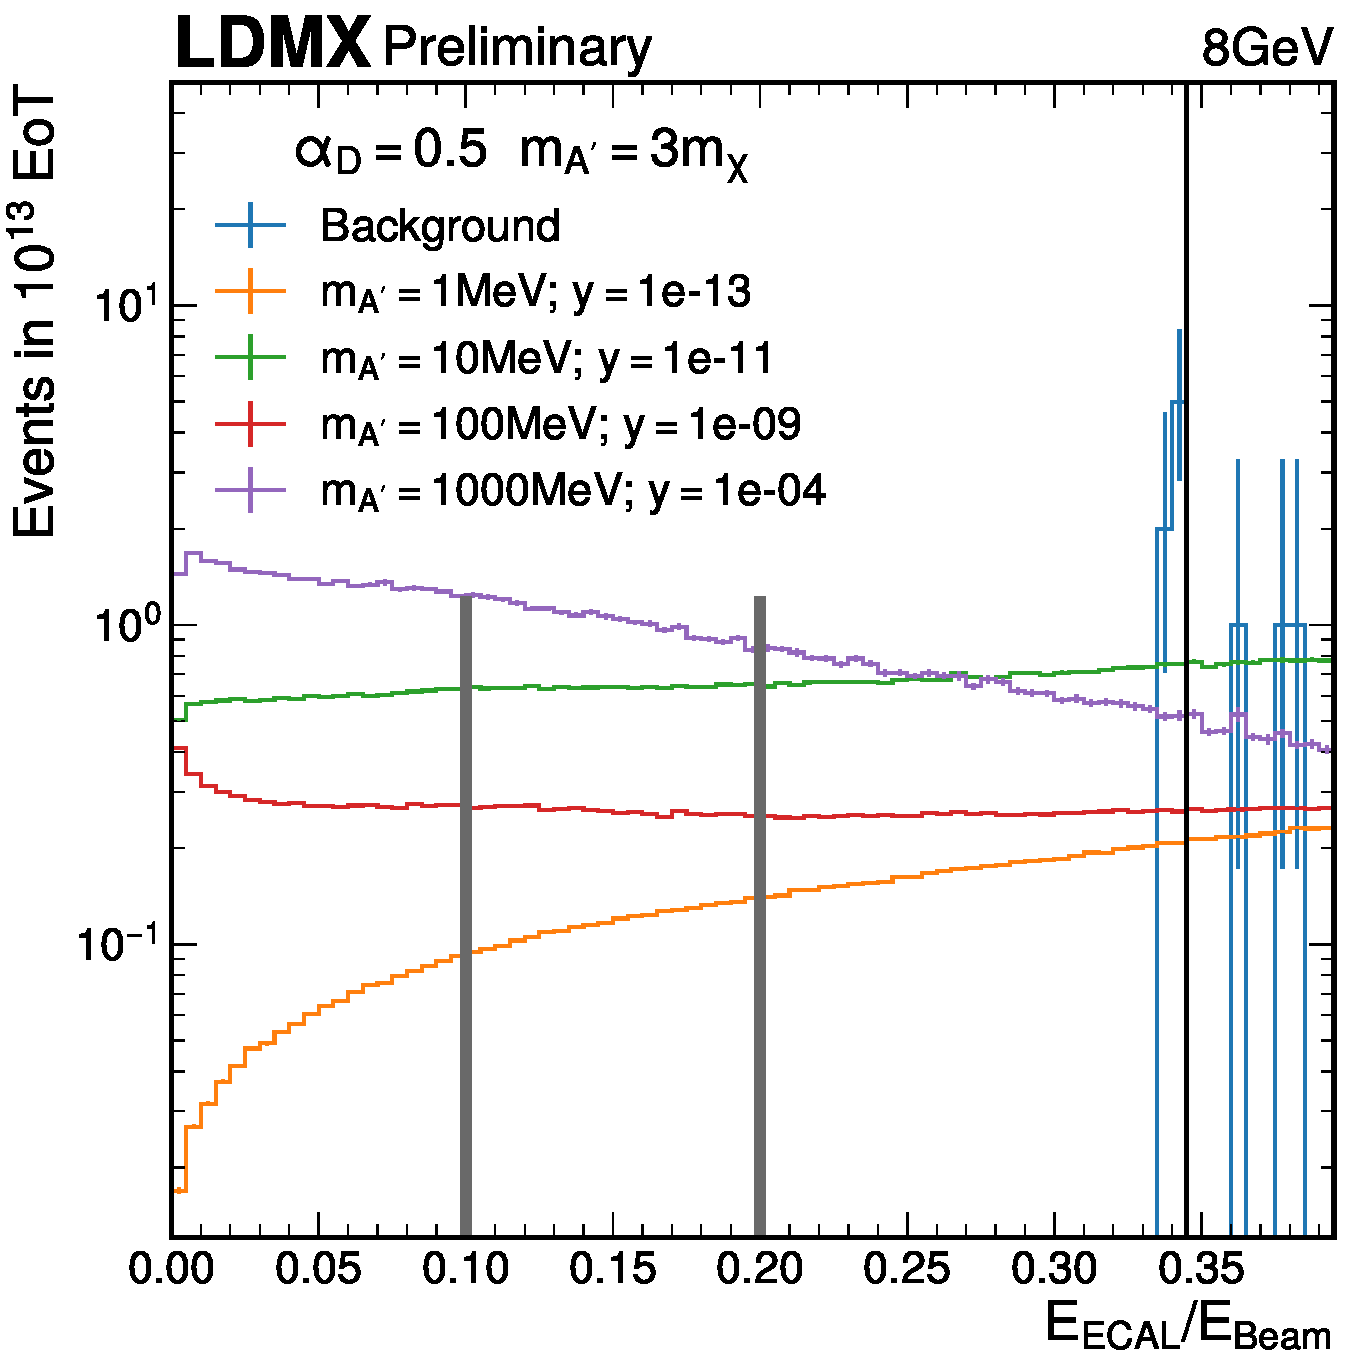
\includegraphics[width=\textwidth]{%
        ../figures/ldmx/analysis/final-selection-with-ana-bin-edges-8gev.pdf}
    \end{column}
    \begin{column}{0.3\textwidth}
      \footnotesize
      \begin{enumerate}
        \item Fit background with simple exponential function
        \item Predict background yield in three channels
        \item Separate signal efficiency into three channels
        \item Include systematic uncertainties for ECal miscalibration
          and HCal PE variation
        \item \textsc{Combine} estimates 95\% CL upper limit on signal
          production yield
      \end{enumerate}
    \end{column}
  \end{columns}
\end{frame}

\note[itemize]{
\item Can still use different shapes between signal and background to our advantage
\item Cut up final energy distribution into three bins (gray lines) with an adjacent
  control region above analysis energy threshold (black line) up to trigger threshold
  (right edge)
\item Signal is roughly evenly distributed across three bins
\item Background is sharply falling
\item Fit with control region to help constrain shape and statistical uncertainties
\item Include systematic uncertainties for ECal miscalibration and HCal PE variation
\item Use \textsc{Combine} statistical tool to estimate 95\% CL median expected limit
  on signal production yield
}

\begin{frame}{Sensitivity in Early Running}
  \begin{columns}
    \begin{column}{0.45\textwidth}
      \begin{figure}
        \centering
        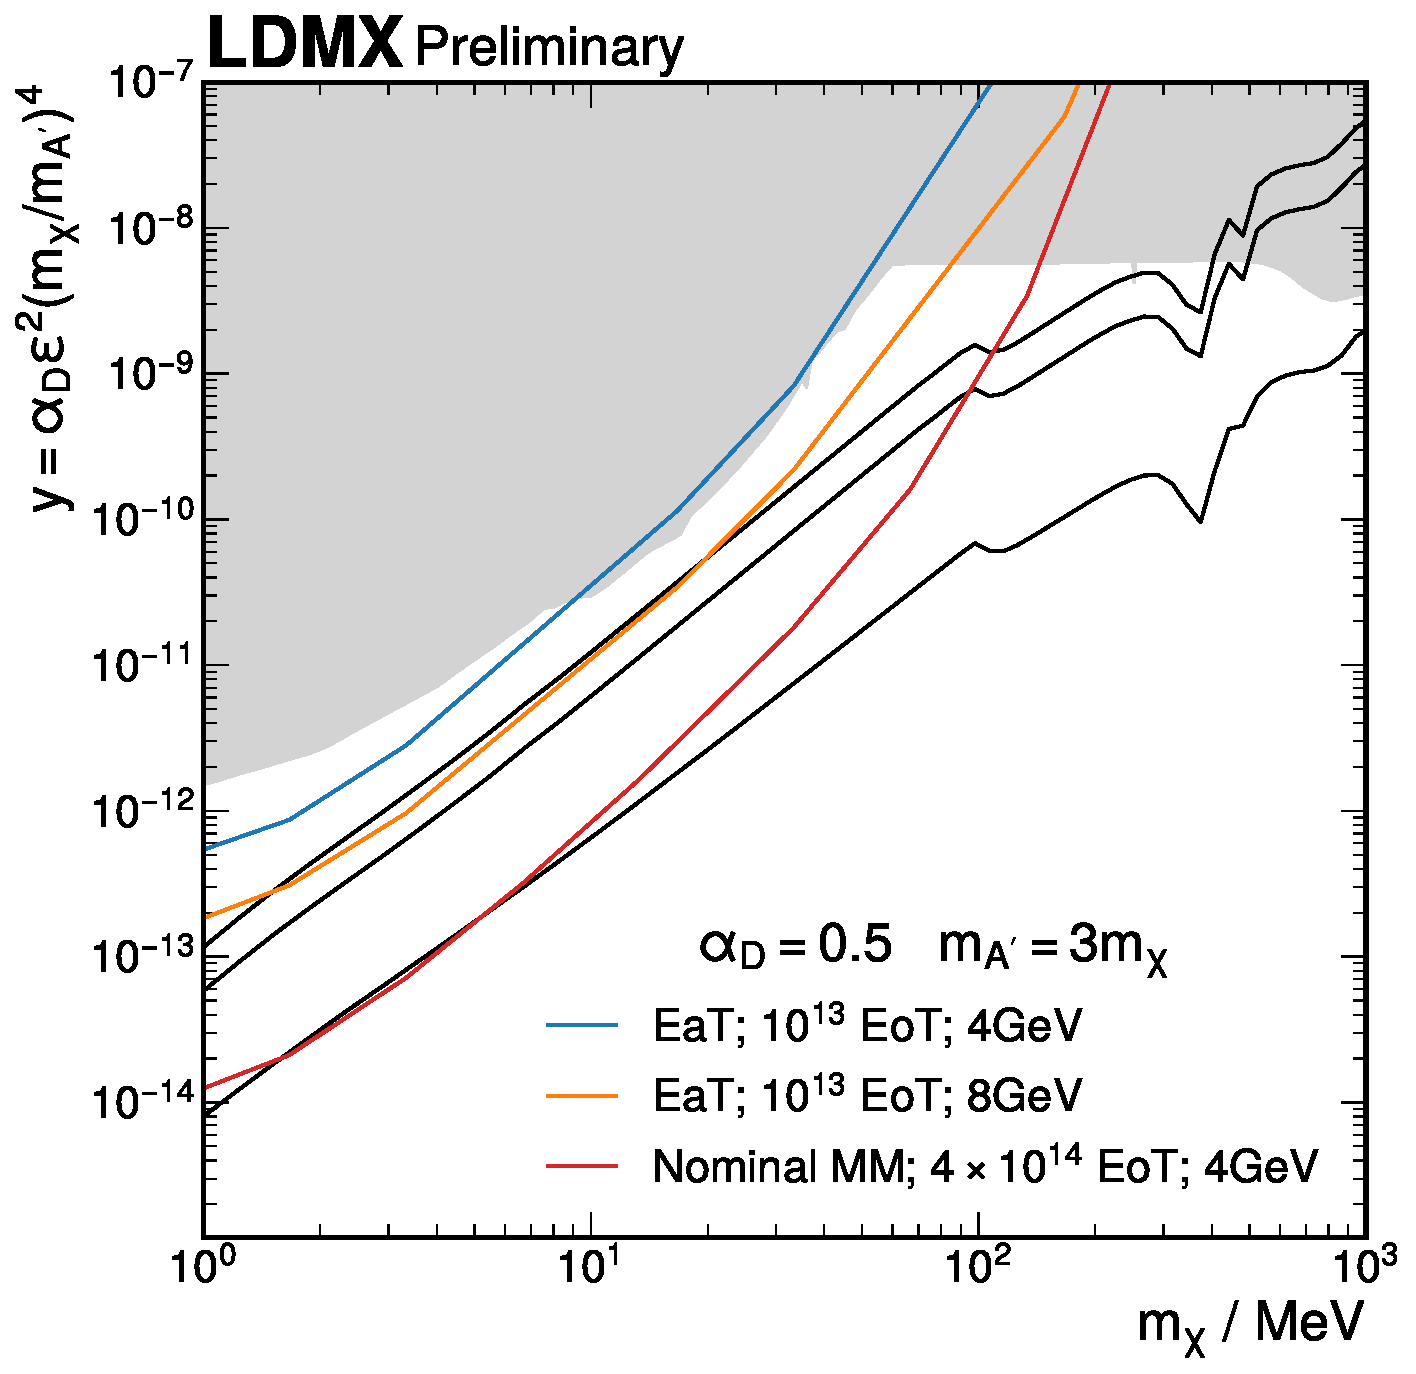
\includegraphics[width=\textwidth]{../figures/ldmx/analysis/reach.pdf}
      \end{figure}
    \end{column}
    \begin{column}{0.55\textwidth}
      \begin{itemize}
        \item For easier comparison, scale upper limit on production yield
          to lower limit on effective interaction strength $y$ using
          estimate of signal production rate
      \end{itemize}
      \vfill 
      \begin{block}{New Territory}
        Able to explore new territory of possible DM while
        learning more about our detector and setting up for
        more data enabling the full nominal analysis.
      \end{block}
    \end{column}
  \end{columns}
\end{frame}

\note[itemize]{
\item Gray is already excluded territory from experiments like NA64, BaBar, and COHERENT
\item Black lines are specific thermal relic theory expectations (From the top: Scalar, Majorana, Pseudo-Dirac)
\item Blue (Orange) is expected limit for this \fourgev (\eightgev) analysis
\item Red is nominal (missing momentum) analysis with 40x more data at \fourgev
}

\ssection{HPS}

\note[itemize]{
\item Heavy Photon Search experiment
\item HPS takes a different approach towards searching for dark brem
\item Instead of looking for extra events with missing energy/momentum,
  we look for extra events with a specific reconstructed quantities
}

\subsection{Experiment}
\begin{frame}{Visible Signature}
  {\color{red}Physics reset, remind of goals}
\end{frame}

\note[itemize]{
\item HPS can throw away a majority of the electrons that don't do anything interesting
\item Searching for highly-displaced electron-positron pairs with specific mass
}

\begin{frame}{Experiment}
  \resizebox{\textwidth}{!}{\begin{tikzpicture}
  \drawhps
\end{tikzpicture}
}
  \vfill
  \begin{columns}
    \begin{column}{0.32\textwidth}
      High rate $\sim\qty{500}{\MHz}$ of incident electrons
    \end{column}
    \begin{column}{0.32\textwidth}
      \qty{15}{mrad} opening angle to avoid detector damage
    \end{column}
    \begin{column}{0.32\textwidth}
      ECal for trigger and energy, SVT for tracks and vertices
    \end{column}
  \end{columns}
\end{frame}

\note[itemize]{
\item HPS installed at Thomas Jefferson Natl Lab
\item Took physics data in 2016, 2019, and 2021 -- scheduled for more data collection in coming years
\item ECal to quickly observe multiple candidate particles and make data collection decision
\item Silicon Vertex Tracker to reconstruct tracks and vertices
\item Benefits
  \begin{itemize}
    \item Physical quantities come with any DM observation
    \item More specific event topology required for standard process to be considered background
  \end{itemize}
\item Downsides
  \begin{itemize}
    \item Need to ``go through'' mixing twice and thus need much higher data volume
    \item Dark sector needs to be ``more defined'' so we can predict
      how it decays back into standard particles
  \end{itemize}
\item Many possible dark sectors yield the correct thermal relic abundance
  simpler one (dark photon returns back to ele-pos pair) has already been searched for
\item Choose one to focus on for further analysis
}

\subsection{Dark Sector Model}
\begin{frame}{Strongly-Interacting Dark Sector}
  \begin{columns}
    \begin{column}{0.6\textwidth}
      \begin{figure}
        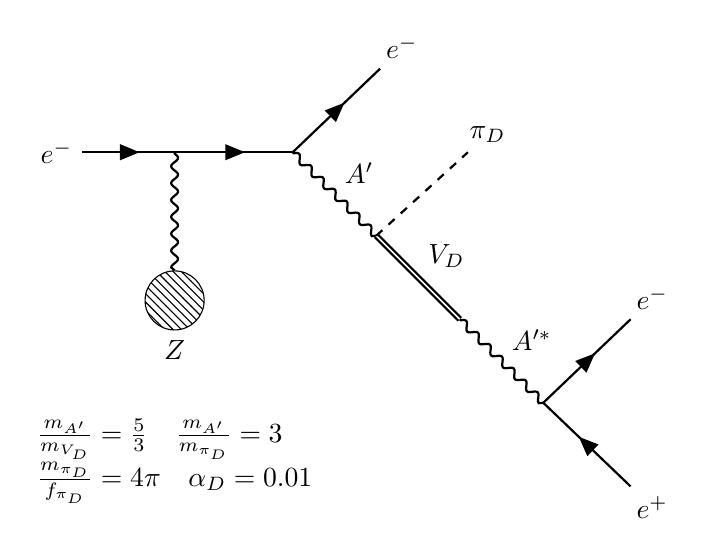
\begin{tikzpicture}
  \begin{feynman}
    \vertex (a) {$e^{-}$};
    \vertex [right= of a](d);
    \vertex [below=of d, blob,label={below:$Z$}] (e) {};
    \vertex [right= of d] (b);
    \vertex [above right= of b] (g) {$e^{-}$};
    \vertex [below right= of b] (aprime_decay);
    \vertex [below right= of aprime_decay] (rhod_decay);
    \vertex [above right= of aprime_decay] (dm) {$\pi_D$};
    \vertex [below right= of rhod_decay] (i);
    \vertex [above right= of i] (j) {$e^{-}$};
    \vertex [below right= of i] (k) {$e^{+}$};
    \diagram*[large] {
    (a) -- [fermion] (d),
    (d) -- [boson] (e),
    (d) -- [fermion] (b),
    (b) -- [fermion] (g),
    (b) -- [boson, edge label={$A'$}] (aprime_decay) -- [double, edge label={$V_D$}] (rhod_decay),
    (aprime_decay) -- [scalar] (dm),
    (rhod_decay) -- [boson, edge label={$A'^*$}] (i),
    (k) -- [fermion] (i) -- [fermion] (j),
    };
  \end{feynman}

  \node [below=of e,align=left] (param)
    {\(\frac{m_{A'}}{m_{V_D}} = \frac{5}{3}\quad\frac{m_{A'}}{m_{\pi_D}} = 3\)\\%
    \(\frac{m_{\pi_D}}{f_{\pi_D}} = 4\pi\quad\alpha_D = 0.01\)};
\end{tikzpicture}

      \end{figure}
    \end{column}
    \begin{column}{0.4\textwidth}
      {\color{UMNMaroon}
      \textbf{S}trongly-\textbf{I}nteracting \\
      \textbf{M}assive \textbf{P}articles
      }
      \begin{itemize}
        \item Dark sector contains ``dark quarks'' -- $\pi_D$ and $V_D$ are mesons like
          standard $\pi$ and $\rho$
        \good Decouples production rate from decay rate
        \bad  Extra missing energy lost to $\pi_D$ during decay chain
      \end{itemize}
      $$
        m_\mathrm{reco} = m_{V_D} \qquad
        z_\mathrm{reco} \sim e^{-z/(c\tau_{V_D})}
      $$
    \end{column}
  \end{columns}
\end{frame}

\note[itemize]{
\item HPS's 2016 dataset is relatively small meaning a simpler dark sector that has
  the dark photon decaying back to electron-positron pair itself was not reachable
\item SIMPs decouple the production and decay rate allowing real sensitivity for HPS
  within this smaller dataset
\item Observables
  \begin{itemize}
    \item[$\to$] Reconstructed mass peaking at dark vector mass
    \item[$\to$] Excess of highly-displaced vertices from decay length of dark vector
  \end{itemize}
\item HPS geometric and trigger acceptance basically requires $A'$ and $V_D$ to be
  colinear with incident electron
  \begin{itemize}
    \item Not difficult for $A'$ since it takes a vast majority of the incident electrons' energy
  \end{itemize}
}

\begin{frame}{Data Collection Trigger}
  \begin{figure}
    \centering
    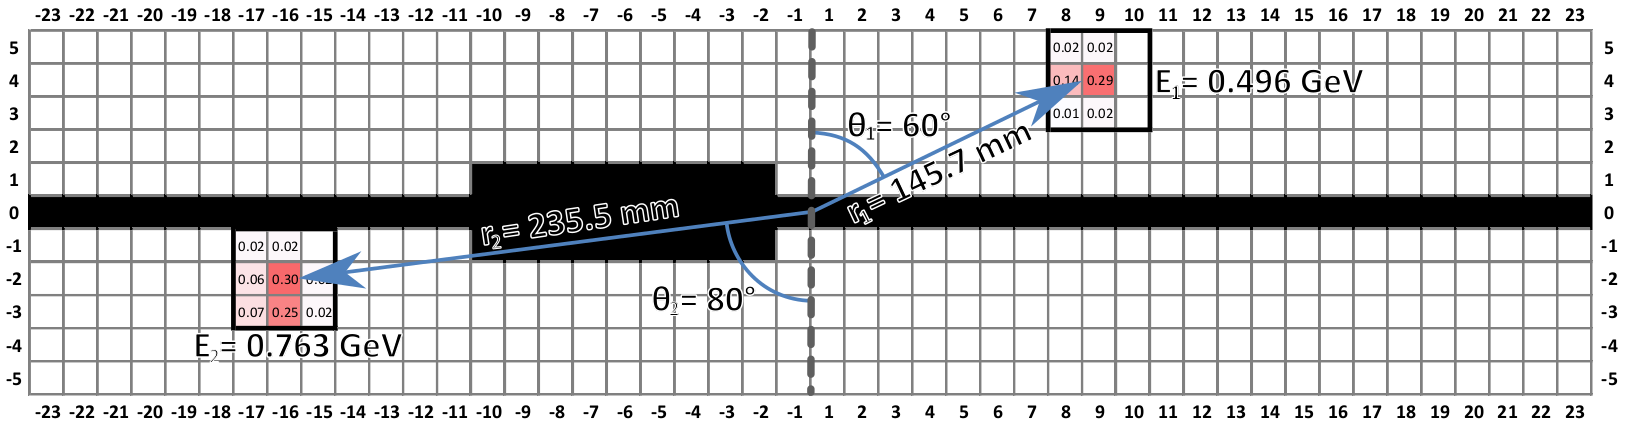
\includegraphics[width=\textwidth]{%
      ../figures/hps/experiment/skmccarty-thesis-fig-27-pair-trigger-depiction.png}
    \caption{Diagram of ECal Pair Trigger. Fig 27 from S K McCarty Thesis 2020.}
  \end{figure}
\end{frame}

\note[itemize]{
\item Credit to SK McCarty for studying and tuning these trigger parameters
\item Individual clusters have at least 2 hits and \qty{0.15}{\GeV} and at most \qty{1.40}{\GeV}
\item Pair energy sum has between \qty{0.6}{\GeV} and \qty{2}{\GeV}
\item Pair energy difference less than \qty{1.14}{\GeV}
\item Low energy cluster matching curvature from magnetic field (roughly)
\item Pair within \qty{35}{\degree} of opposite
}

\begin{frame}{Preliminary Quality Selections}
  \begin{columns}
    \begin{column}{0.35\textwidth}
      \centering
      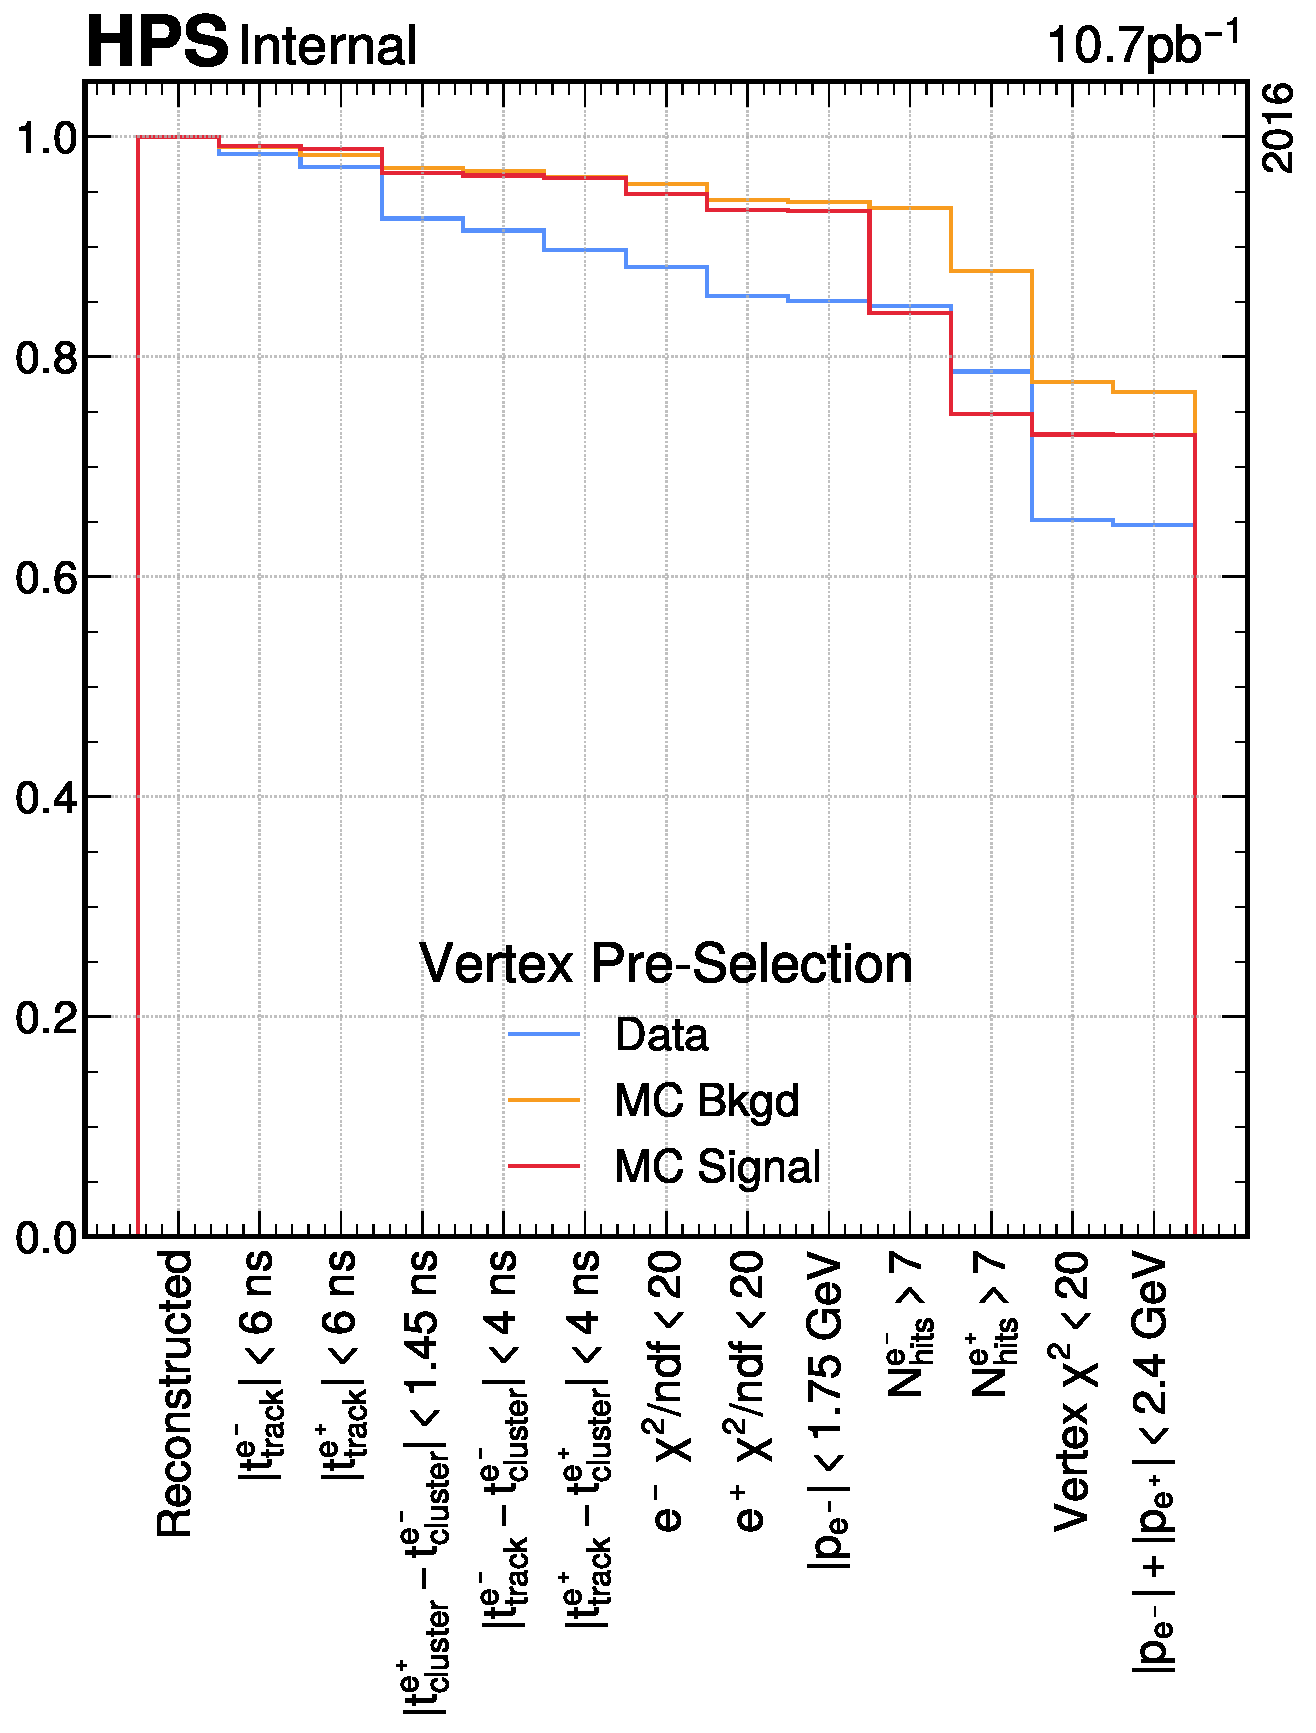
\includegraphics[width=\textwidth]{%
        ../figures/hps/dataset/vertex-pre-selection-efficiency.pdf}
    \end{column}
    \begin{column}{0.3\textwidth}
      Count number of vertices passing the
      quality selections
    \end{column}
    \begin{column}{0.35\textwidth}
      \centering
      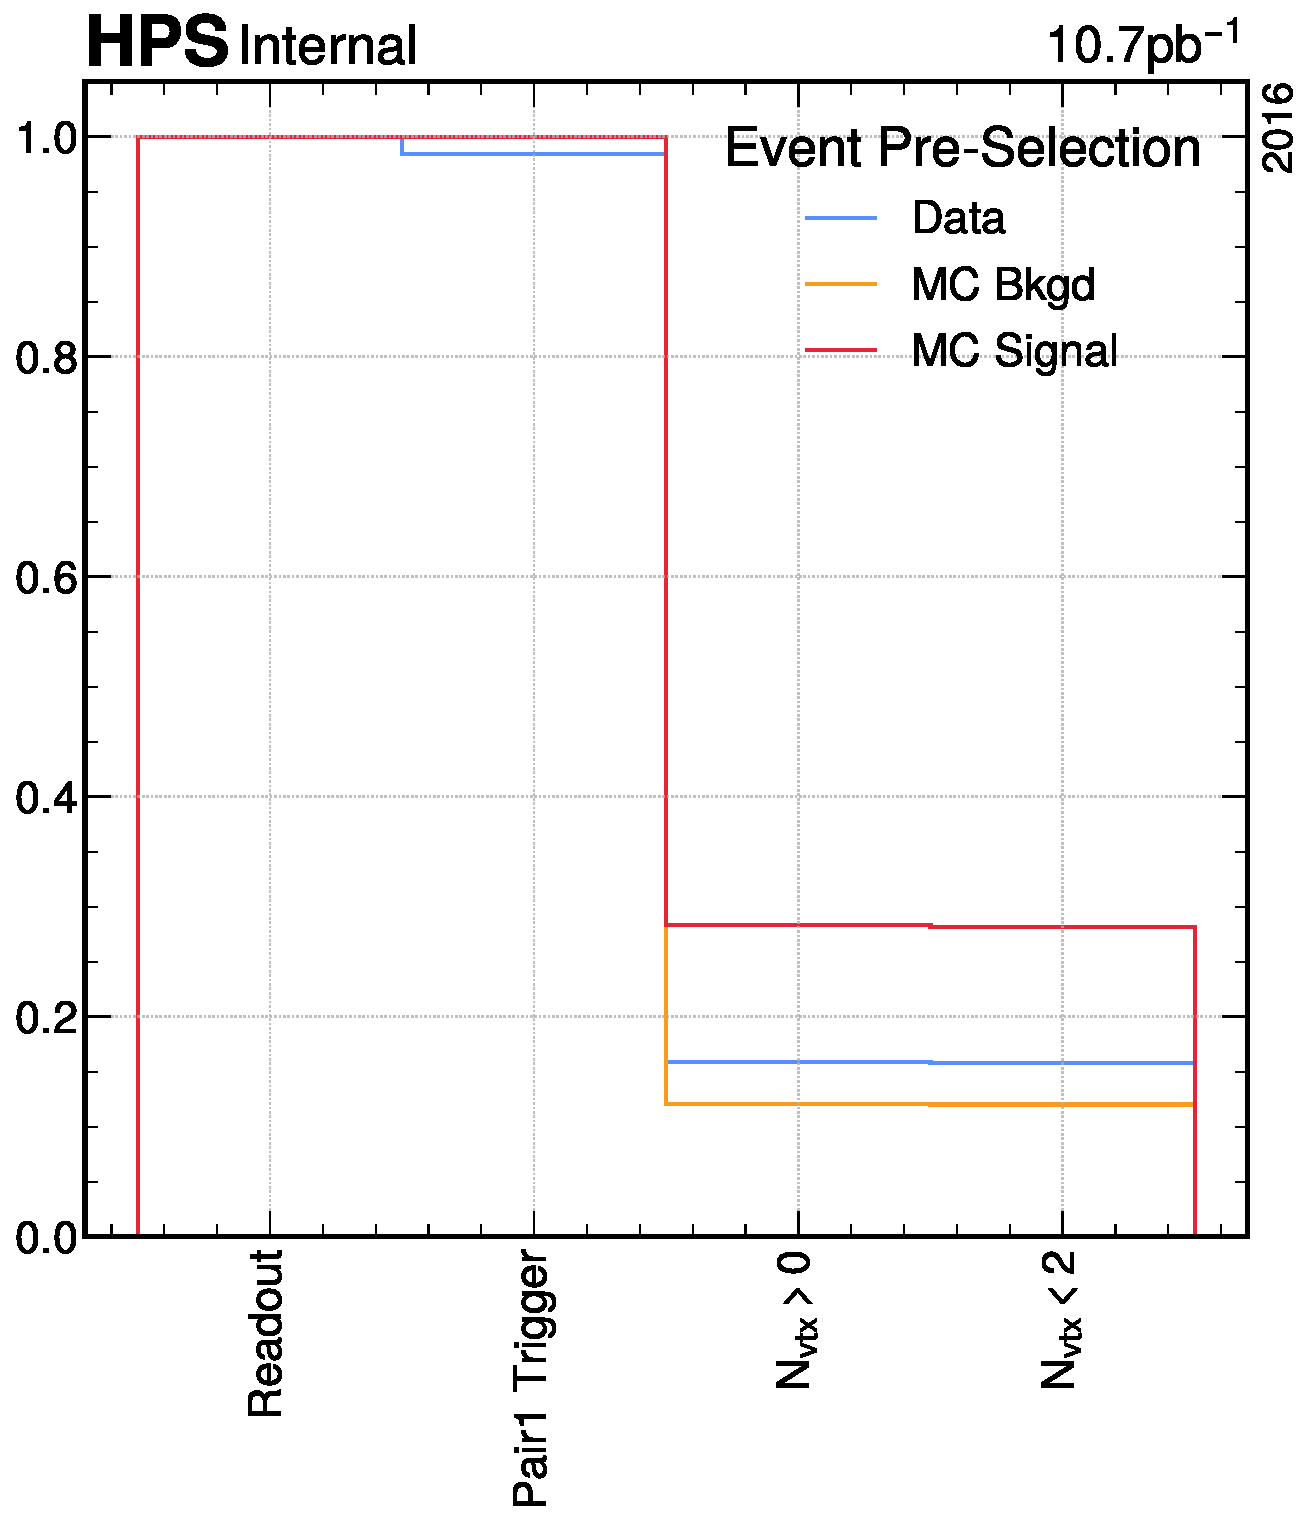
\includegraphics[width=\textwidth]{%
        ../figures/hps/dataset/event-pre-selection-efficiency.pdf}
    \end{column}
  \end{columns}
\end{frame}

\note[itemize]{
\item After this trigger selection, we apply some more selections to focus
  on higher quality vertices
\item Credit to A Spellmen for studying and tuning this pre-selection
\item Requirement that a vertex is reconstructed is biggest difficulty,
  reflects (roughly) the geometric acceptance of the detector
\item Onto a few more detailed selections focused on separating signal from background
}

\subsection{Orthogonal Reconstruction Categories}
\begin{frame}{L1L1 and L1L2}
  \begin{columns}
    \begin{column}{0.3\textwidth}
      \resizebox{\textwidth}{!}{\begin{tikzpicture}
  \drawhpsfirsttwolayers
  \node at (\targetx,+2) {L1L1};
  \node at (\targetx+1,0.1) [circle,fill,inner sep=1.5pt] {};
  \draw[black,->] (\targetx+1,0.1) -- (2.5,2) node[anchor=north west] {\(e^-\)};
  \draw[black,->] (\targetx+1,0.1) -- (2.5,-1.9) node[anchor=south west] {\(e^+\)};
\end{tikzpicture}
}
      \resizebox{\textwidth}{!}{\begin{tikzpicture}
  \drawhpsfirsttwolayers
  \node at (\targetx,+2) {L1L2};
  \node at (\targetx+2.0,0.1) [circle,fill,inner sep=1.5pt] {};
  \draw[black,->] (\targetx+2.0,0.1) -- (2.5,2) node[anchor=north west] {\(e^-\)};
  \draw[black,->] (\targetx+2.0,0.1) -- (2.5,-1.8) node[anchor=south west] {\(e^+\)};
\end{tikzpicture}
}
    \end{column}
    \begin{column}{0.6\textwidth}
      Quality of reconstruction is closely tied with how many (and which)
      tracker layers are hit.
      \begin{itemize}
        \item Helpful to separate analyses into reconstruction categories
      \end{itemize}
      \vfill
      \begin{block}{Orthogonal Analyses}
        Experiment design categories (should) have no effect on observable
        physics so they are helpful cross checks for each other.
      \end{block}
    \end{column}
  \end{columns}
\end{frame}

\note[itemize]{
\item \textit{Quality -- Categories}
\item L1L1 requires all four sensors in first two layers to have hits for both tracks
\item L1L2 drops the first layer requirement for only one of the tracks
\item L1L2 vertices are more ``contaminated'' but also reach to higher displacements
}

\begin{frame}{Basic, Fixed Selection}
  \begin{itemize}
    \item \boldcol{UMNSunny}{L1L2}: In the vertex, one of the particles 
      must have a hit in both sensors in Layer 1 and Layer 2
      while the other must have a hit in both sensors in Layer 2 and Layer 3.
      \begin{itemize}
        \item The reconstruction category I am studying
      \end{itemize}
    \item \boldcol{UMNSunny}{Low Momentum Sum}:
      $\qty{1.0}{\GeV} < P_\mathrm{sum} < \qty{1.9}{\GeV}$
      \begin{itemize}
        \item Missing energy ``lost`` to $\pi_D$
      \end{itemize}
    \item \boldcol{UMNSunny}{Decay after Target}: $z > z_\mathrm{target}$
      \begin{itemize}
        \item Redundant with the \minyzero cut, but ensures decay weights
          don't unphysically diverge
      \end{itemize}
    \item \boldcol{UMNSunny}{Mass Window}: $p_m < 2.8$ (exclusion), $p_m < 1.5$ (search SR),
      $1.5 < p_m < 4.5$ (search sideband)
      \begin{itemize}
        \item electron-positron pair has mass within resolution of $V_D$ test mass
      \end{itemize}
  \end{itemize}
  $$
    p_m = \frac{|m_\mathrm{reco}-m_{V_D}|}{\sigma_m}
  $$

  \begin{block}{Optimization}
    Optimize further cuts on 10\% subsample of data
  \end{block}
\end{frame}

\note[itemize]{
\item The L1L1 category, consisting of higher-quality vertices, has already
  been studied, helpfully optimizing many selections that are easily applicable
  to the L1L2 category as well
\item \textit{Selections}
\item Using sub-sample of data in order to avoid background simulation that
  is not trustworthy
}

\subsection{Cut Optimization Procedure}
\begin{frame}{Helpful Physics Variables}
  \begin{columns}
    \begin{column}{0.3\textwidth}
      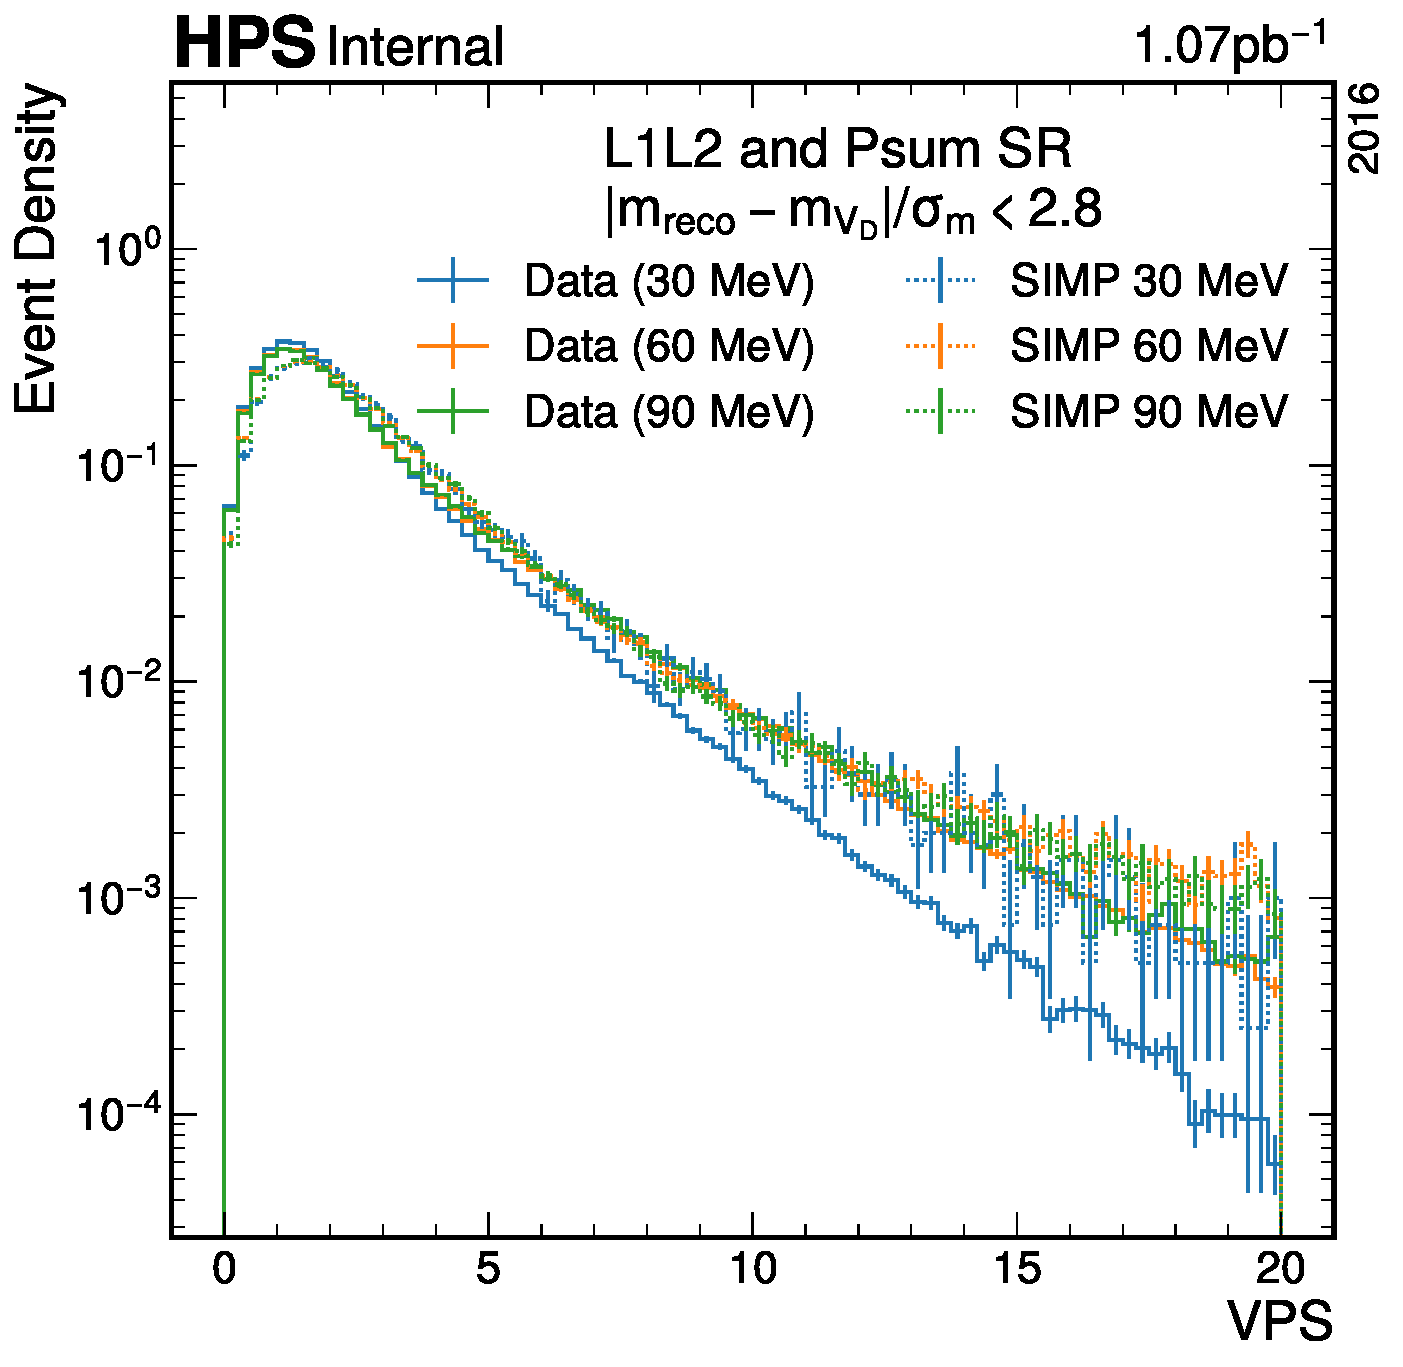
\includegraphics[width=\textwidth]{%
        ../figures/hps/analysis/vtx_proj_sig-distribution.pdf}
      \ac{vps} measures how close vertex
      is to originating from beam spot
    \end{column}
    \begin{column}{0.3\textwidth}
      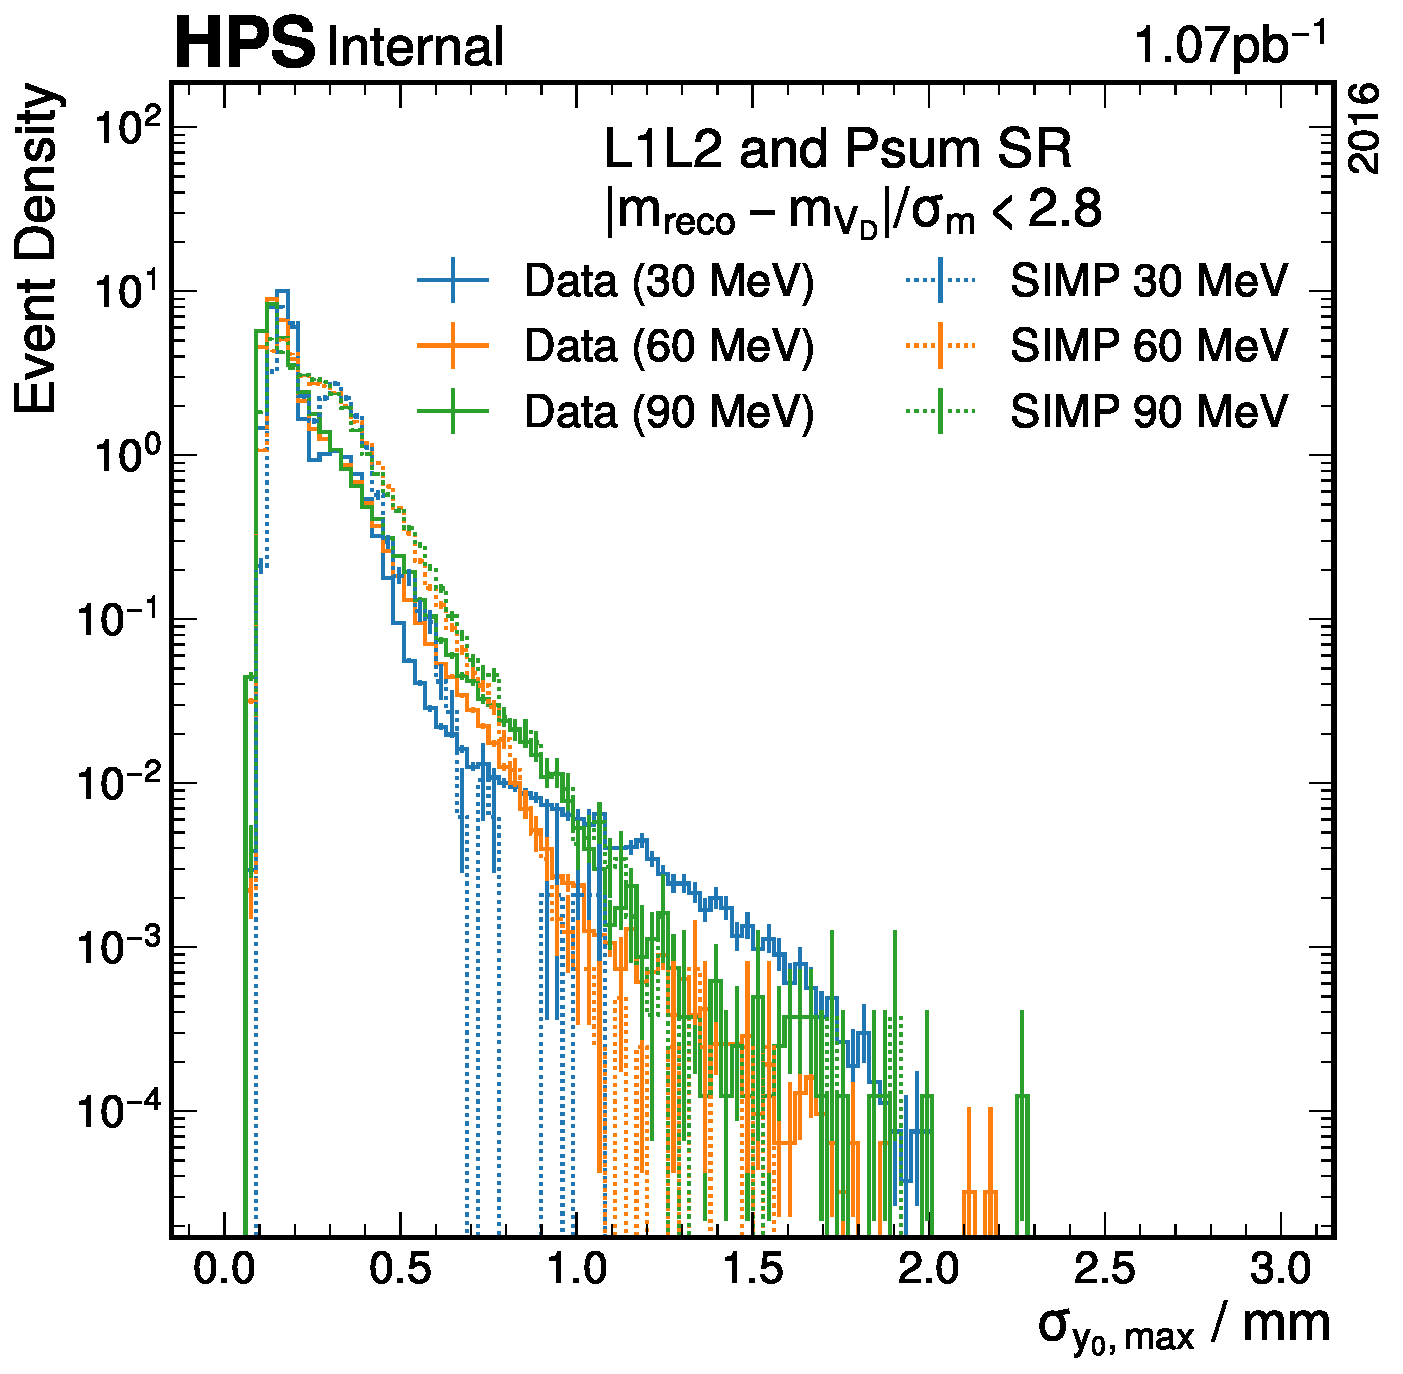
\includegraphics[width=\textwidth]{%
        ../figures/hps/analysis/max_y0_err-distribution.pdf}
      \maxyzeroerr requires high precision
      of vertical impact parameter
    \end{column}
    \begin{column}{0.3\textwidth}
      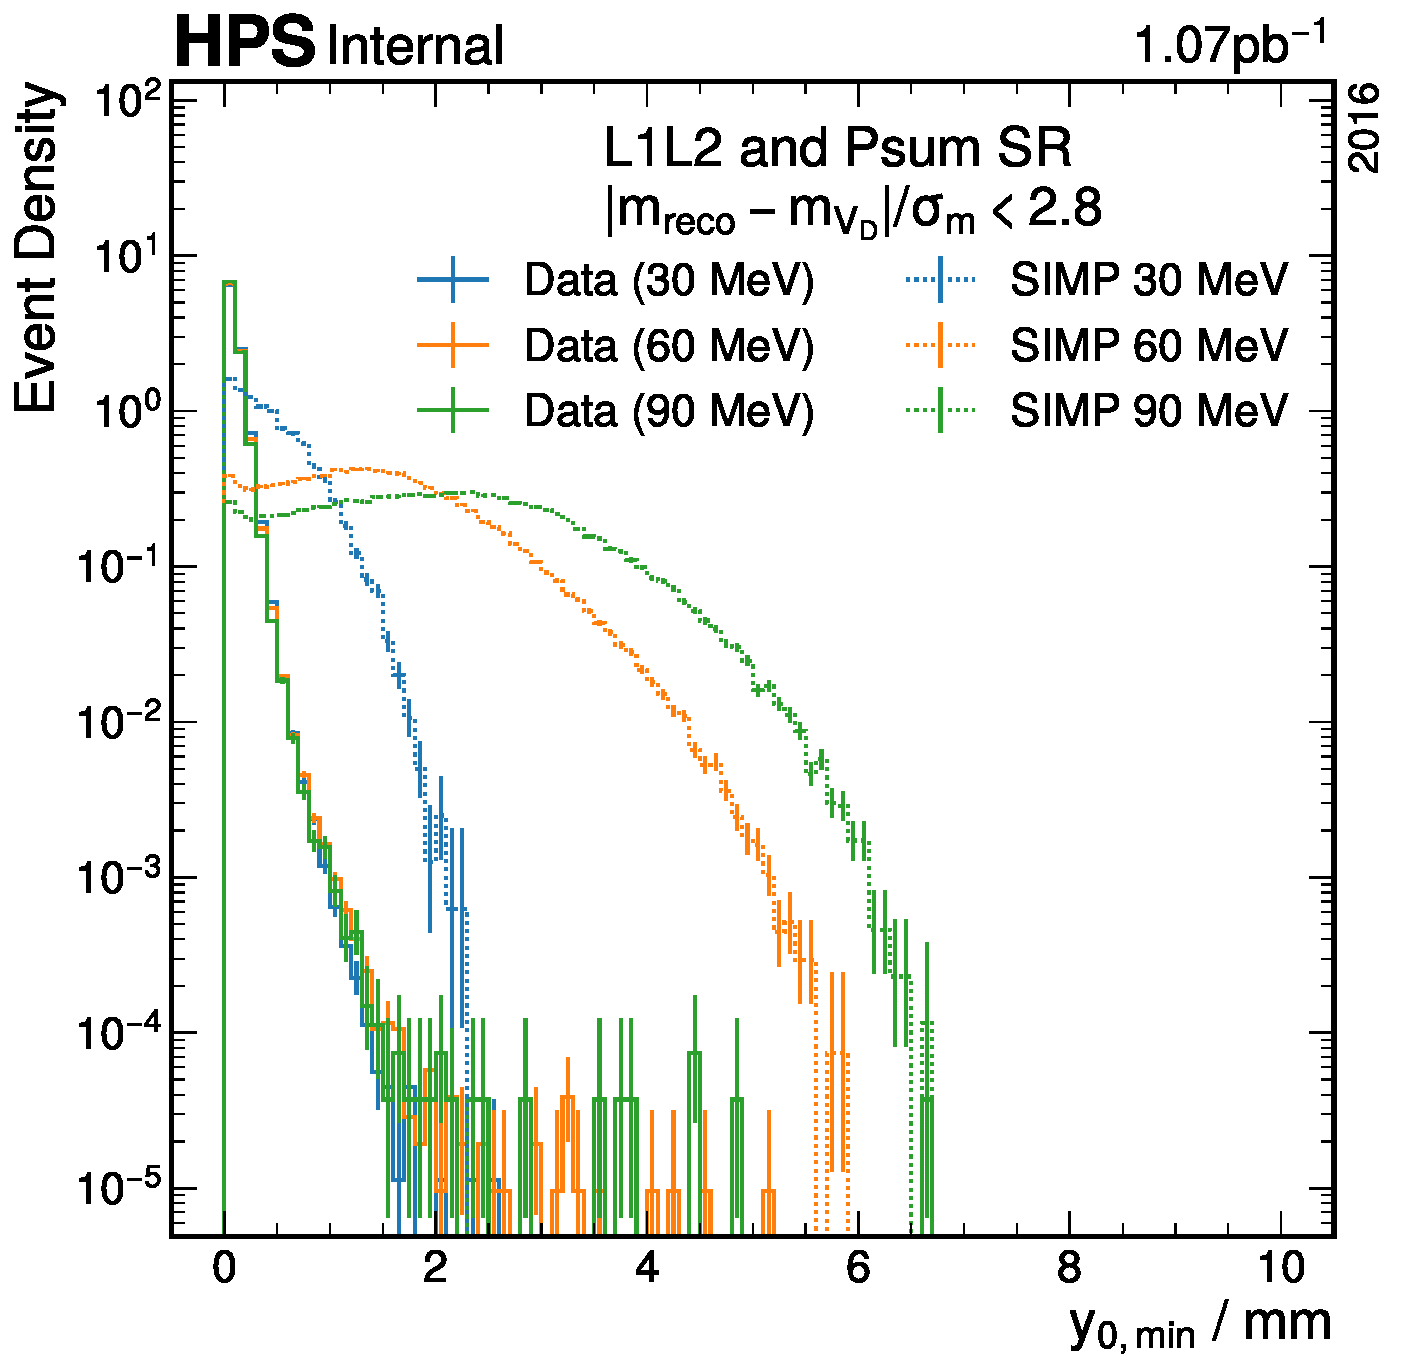
\includegraphics[width=\textwidth]{%
        ../figures/hps/analysis/min_y0-distribution.pdf}
      \minyzero separates signal and background
      with better resolution compared to others
      (like $z$ for example)
    \end{column}
  \end{columns}
\end{frame}

\note[itemize]{
\item Searching the data has shown these variables to provide help separating
  signal and background
\item Two additional quality requirements (\ac{vps} and \maxyzeroerr) followed by
  \minyzero separation
}

\begin{frame}{Optimization Procedure}
  \begin{columns}
    \begin{column}{0.3\textwidth}
      {Keep relative signal efficiency high ($> \qty{80}{\%}$)
      while trimming data tail of \minyzero distribution.}
      
      \vfill

      {
      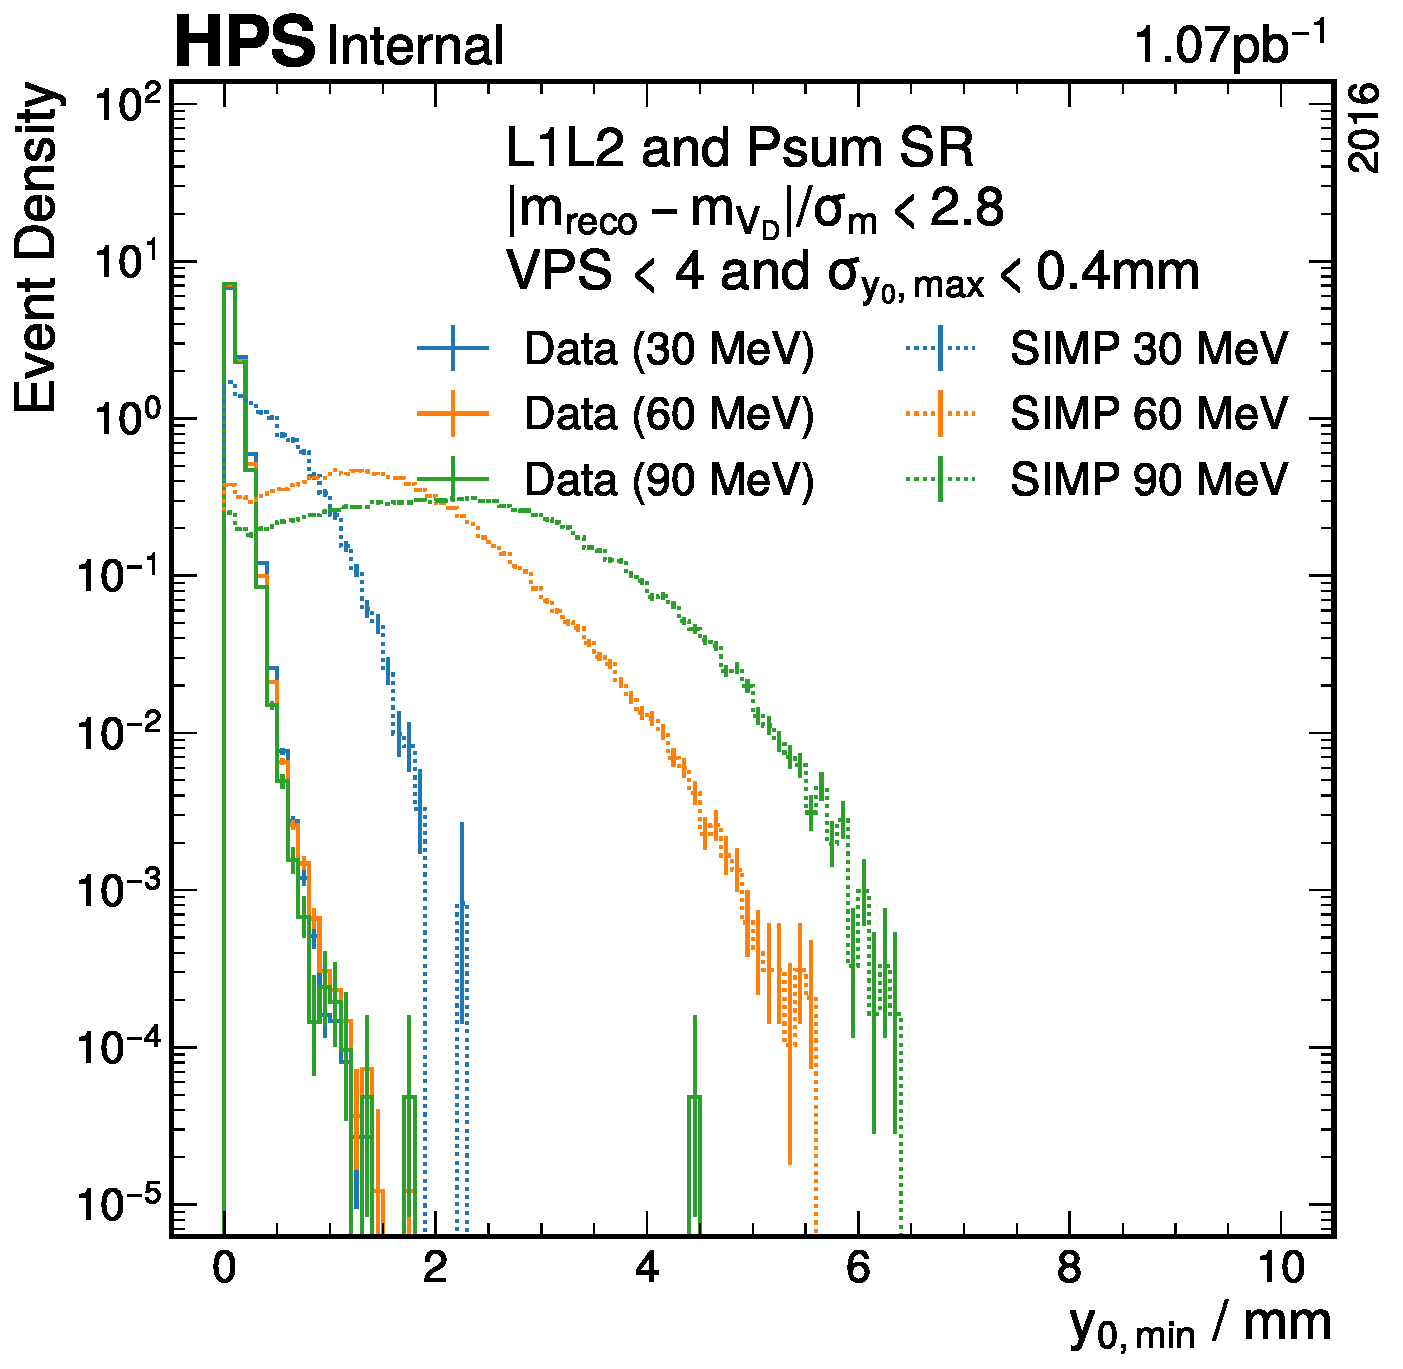
\includegraphics[width=\textwidth]{%
        ../figures/hps/analysis/min-y0-after-others.pdf}
      }
    \end{column}
    \begin{column}{0.69\textwidth}
      \begin{block}{Binomial Significance}
        Maximize binomial significance $Z_\mathrm{Bi}$
        within core mass region with best sensitivity
        and then smooth with a linear fit.
      \end{block}
      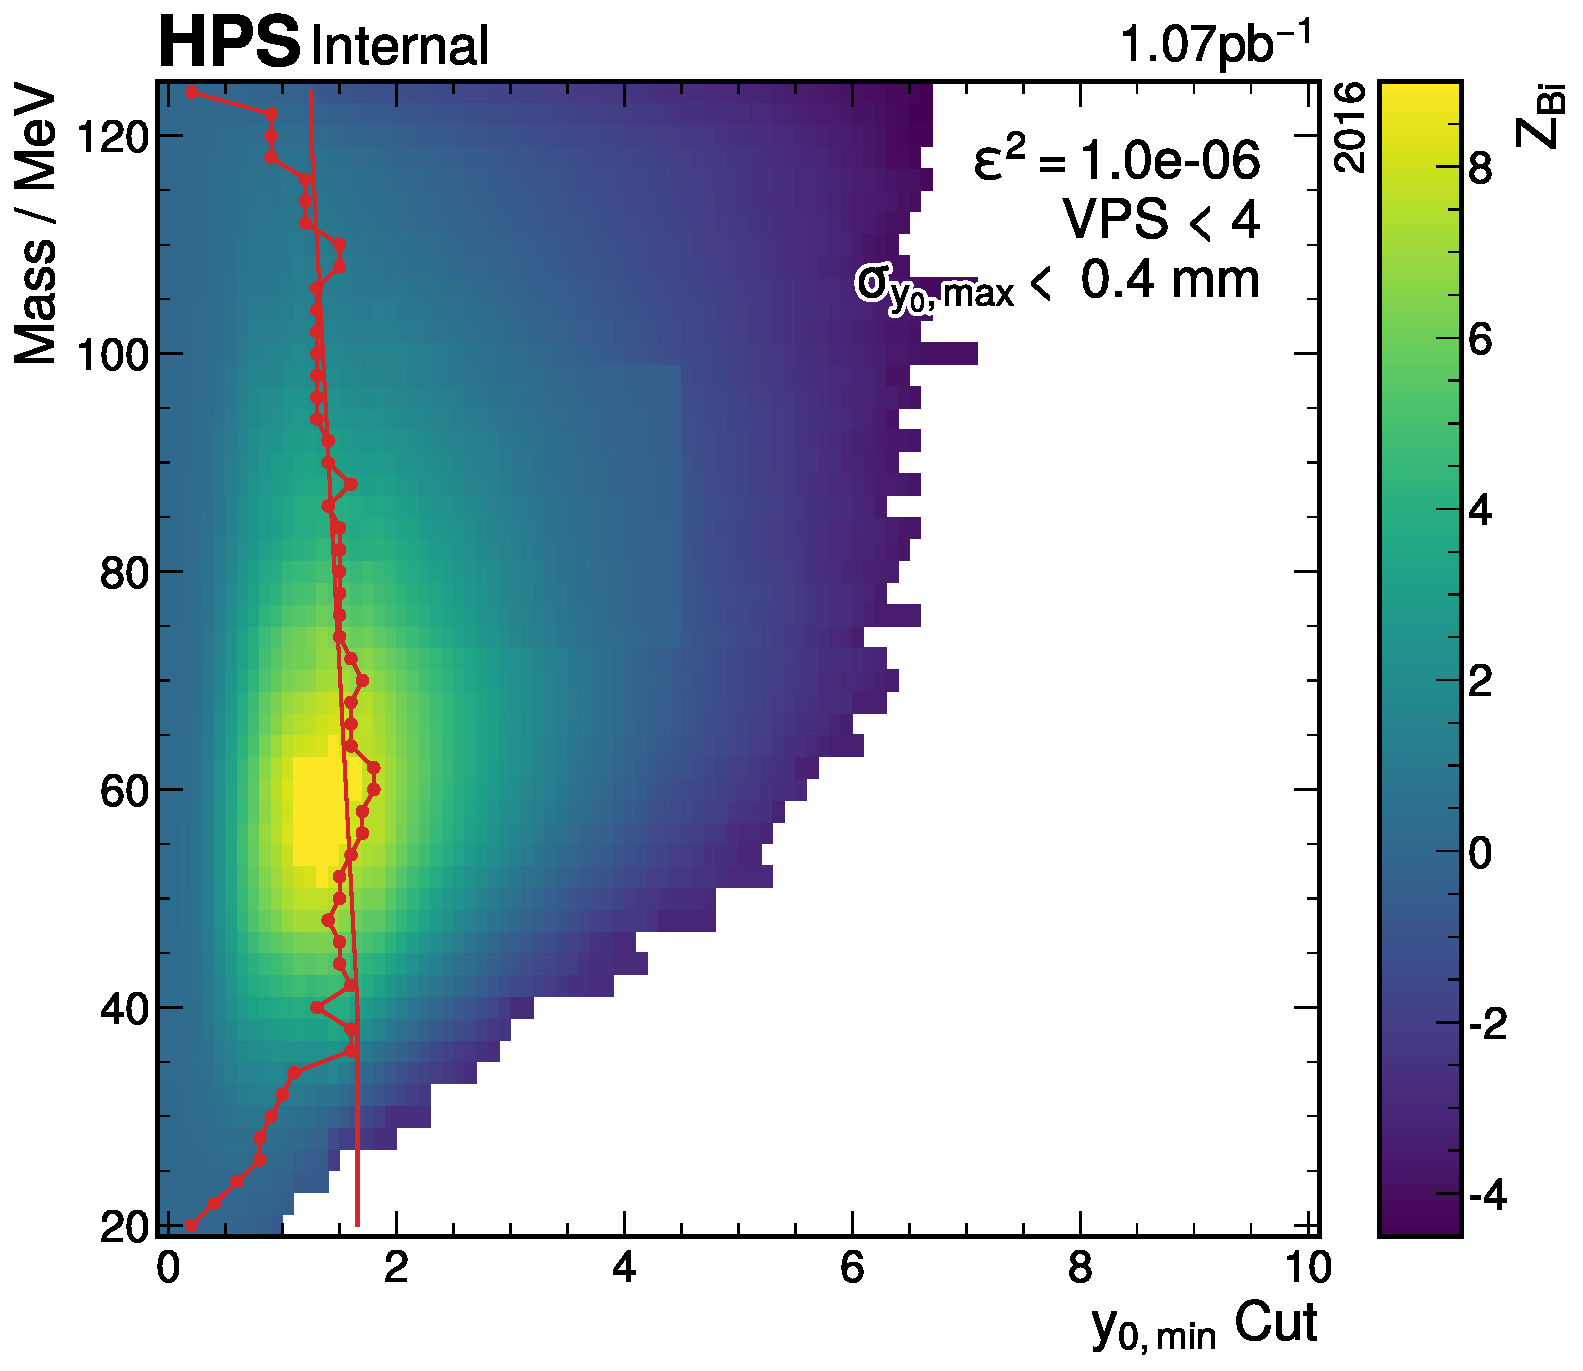
\includegraphics[width=0.48\textwidth]{%
        ../figures/hps/analysis/miny0-after-others-zbi-eps2-1e-6.pdf}
      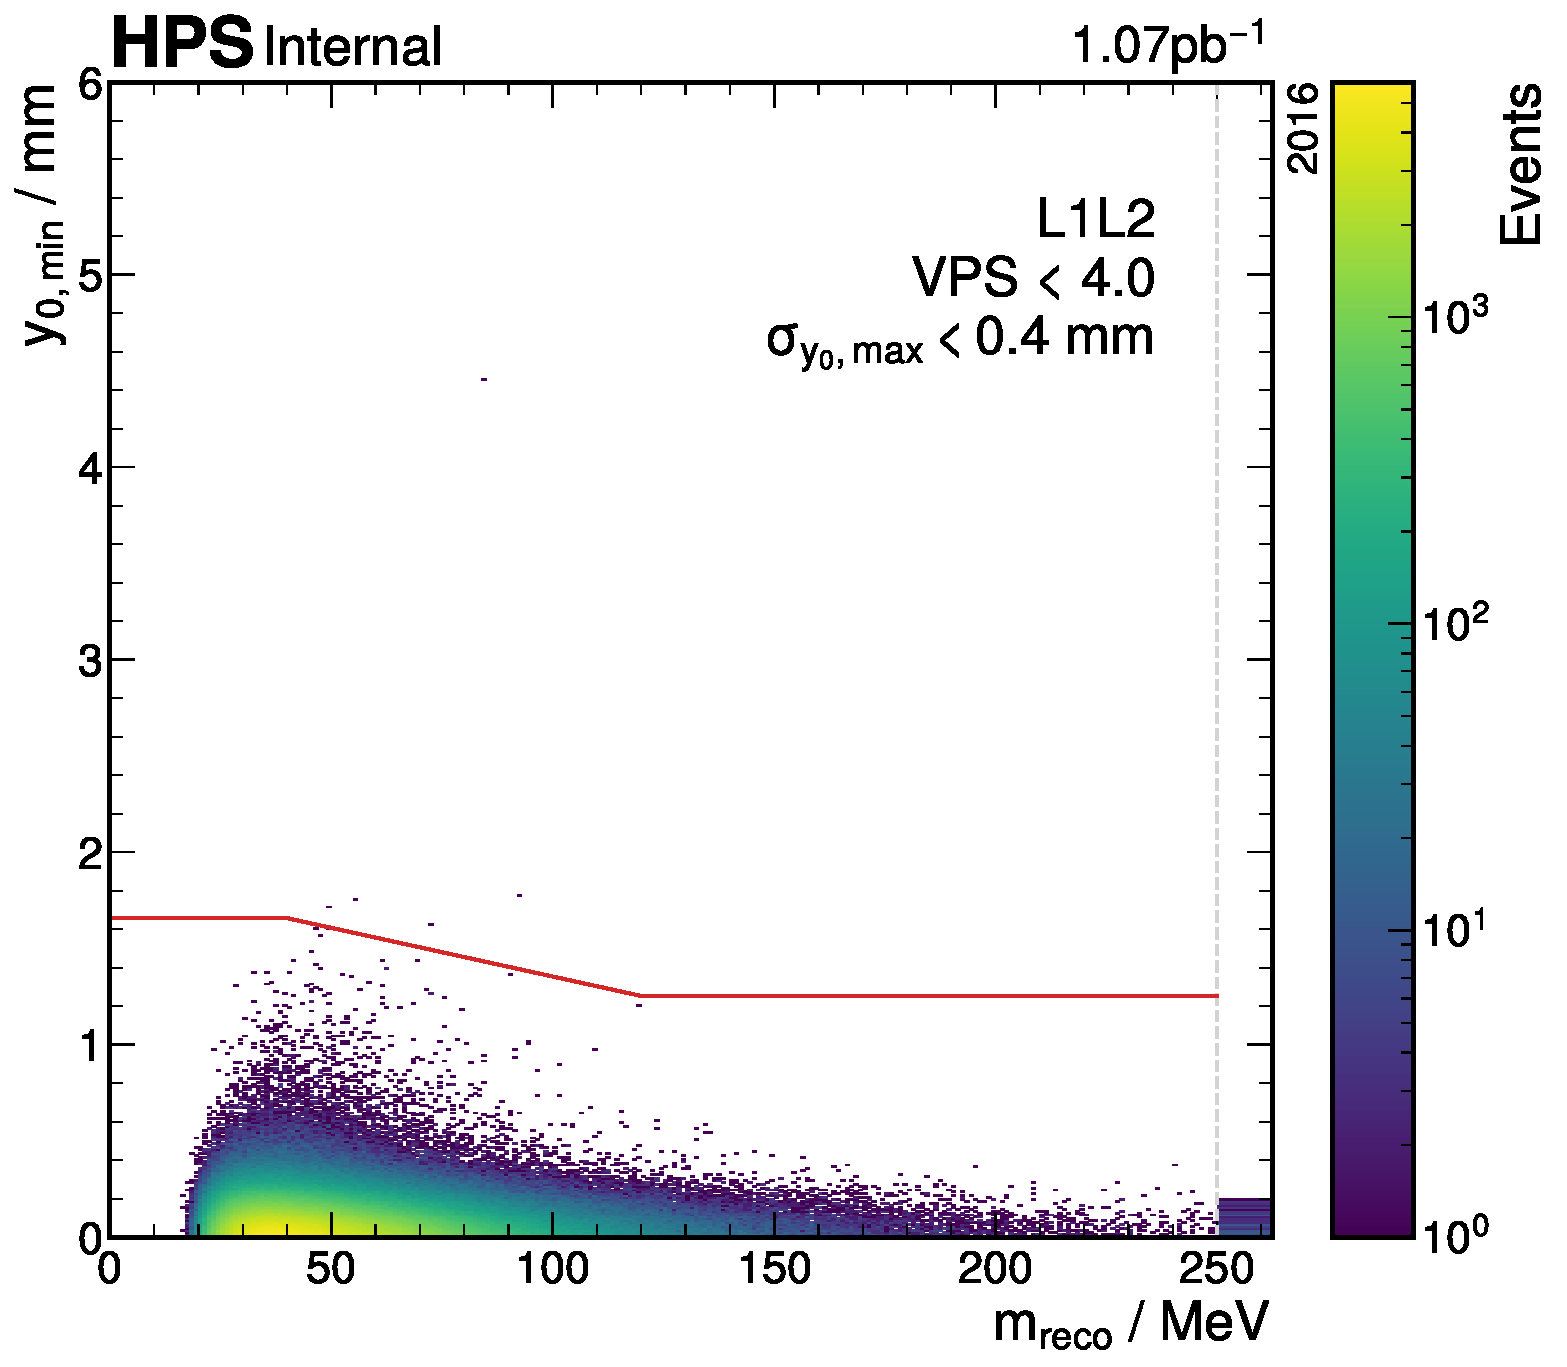
\includegraphics[width=0.48\textwidth]{%
        ../figures/hps/analysis/results/y0-cut-on-data.pdf}
    \end{column}
  \end{columns}
\end{frame}

\note[itemize]{
\item Trim the data tail of the \minyzero distribution while keeping the signal efficiency
  high
\item After some searching and double-checking, landed on \ac{vps} $< 4$
  and \maxyzeroerr$< \qty{0.4}{\mm}$
\item After these additional quality cuts, we then focus on maximizing the binomial
  significance of the hypothetical signal on top of the background distribution
  \begin{itemize}
    \item Signal yield needed to be artificially scaled so that it was on the same
      order of magnitude as the observed data
    \item Varying this scale did not alter the chosen cuts except in extreme cases
  \end{itemize}
\item The cuts maximizing the $Z_\mathrm{Bi}$ are then smoothed with a linear fit
  to help alleviate statistical bias
\item \minyzero cut extending outside of the fit range with a flat value
\item Undergoing internal HPS review of this selection right now,
  only show results from 10\% subsample since I have not been approved to unblind yet
}

\subsection{Results}

\begin{frame}{Search}
  \begin{columns}
    \begin{column}{0.45\textwidth}
      \centering
      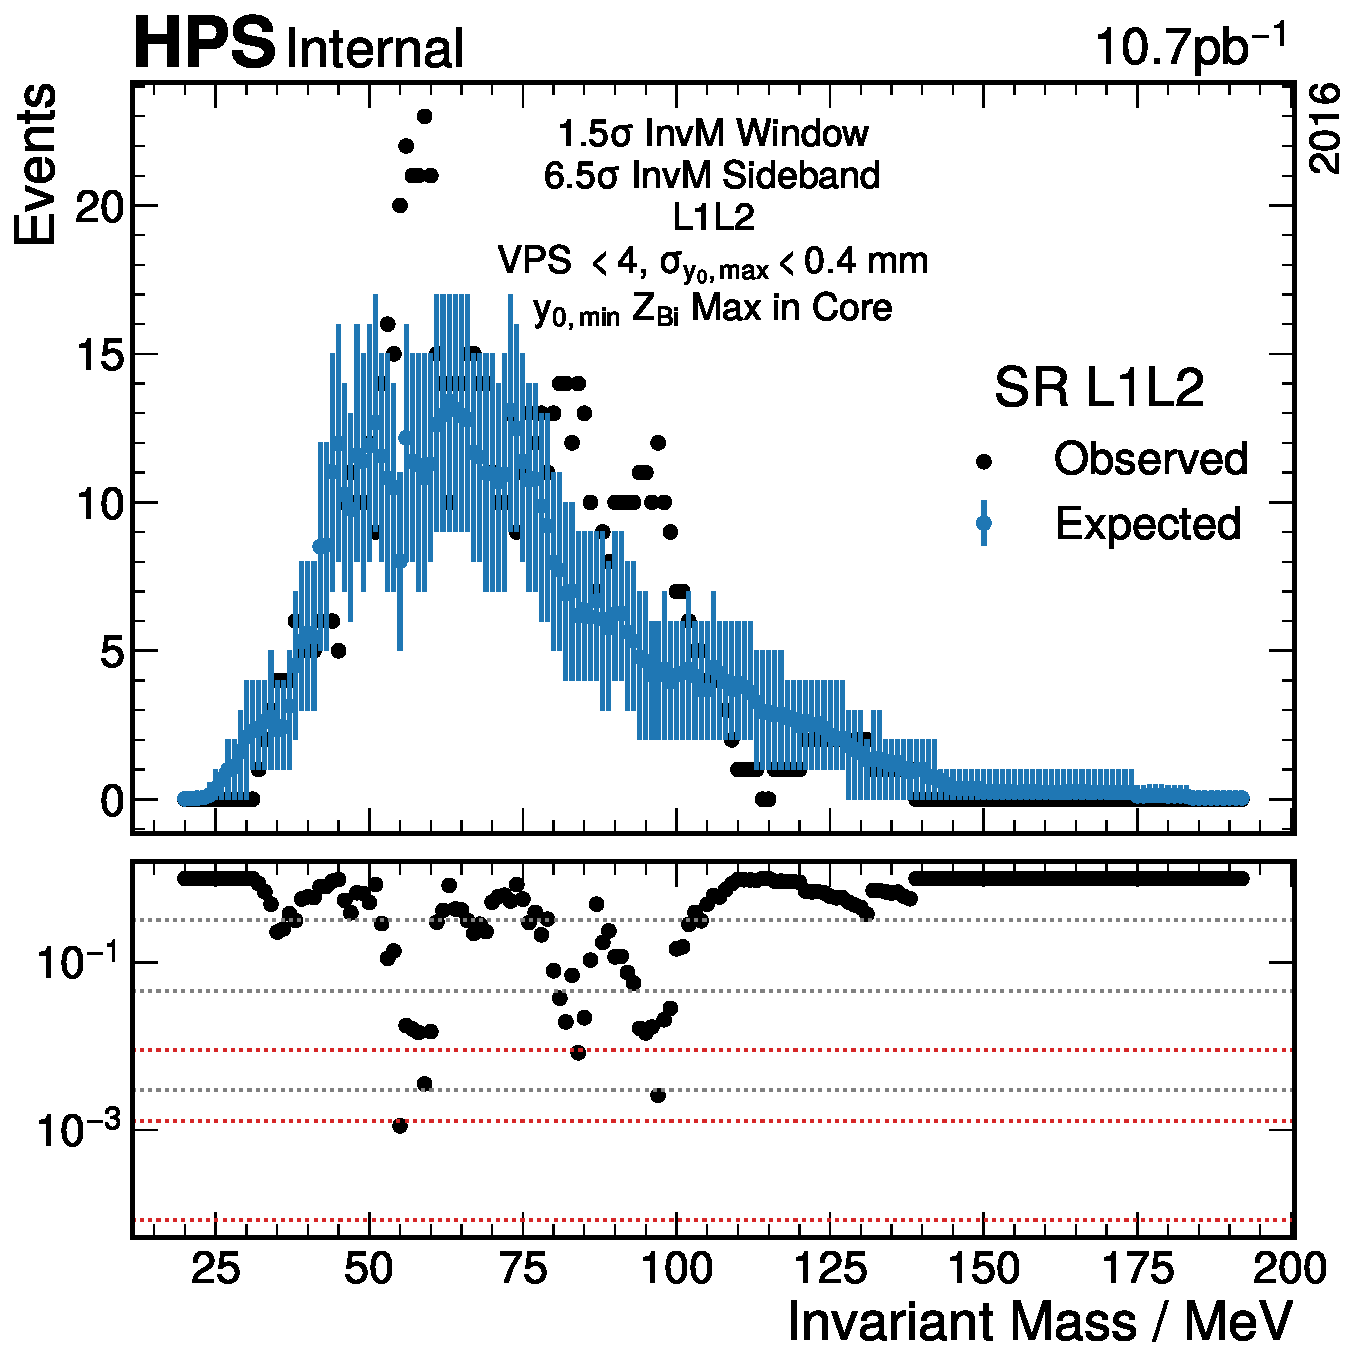
\includegraphics[width=\textwidth]{../figures/hps/analysis/results/search.pdf}
    \end{column}
    \begin{column}{0.55\textwidth}
      \centering
      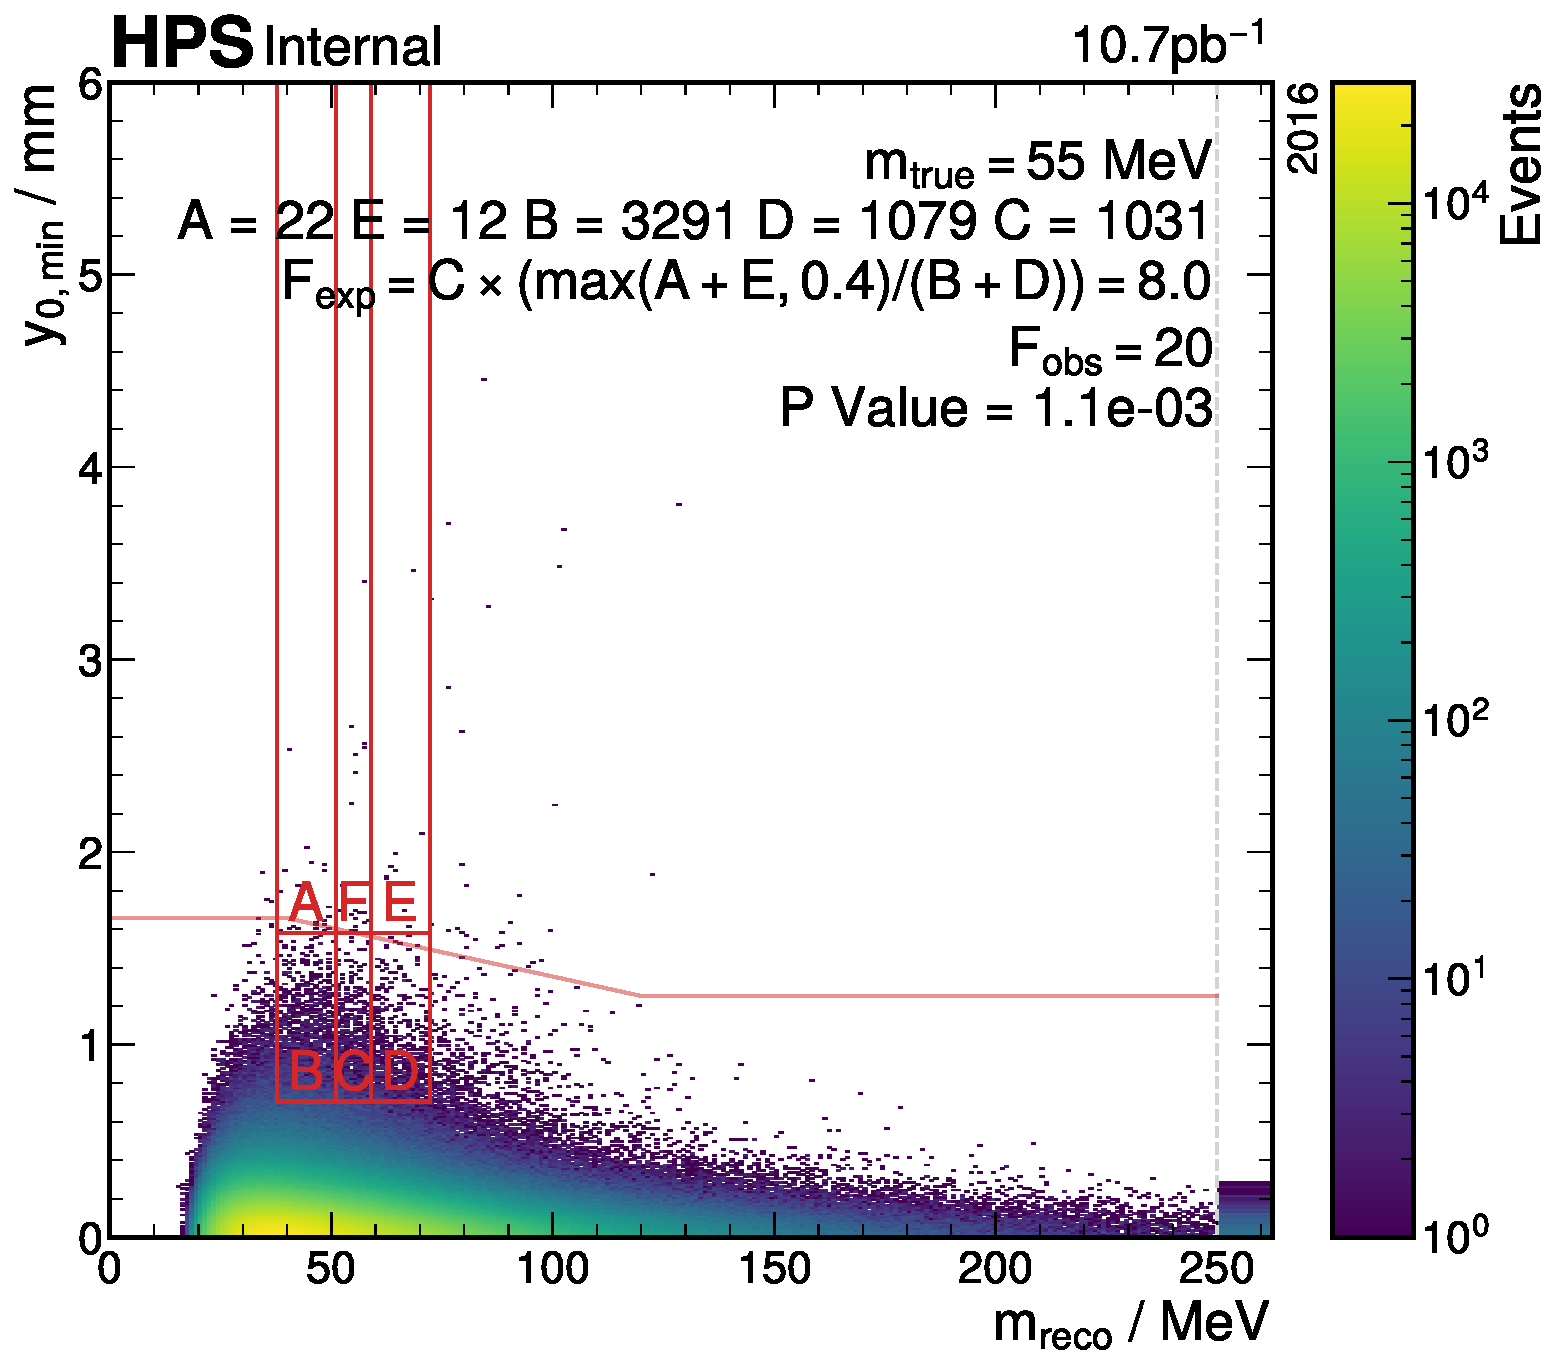
\includegraphics[width=\textwidth]{../figures/hps/analysis/results/search-min-p-val.pdf}
    \end{column}
  \end{columns}
\end{frame}

\note[itemize]{
\item Search for excess in mass-displacement space using a modified ABCD approach
\item Do not observe any excess exceeding one sigma global significance (red lines)
  within the 10\% subsample used for cut optimization
\item No excess $\to$ move to exclusion
}

\begin{frame}{Expected Sensitivity from 10\% Subsample}
  \begin{columns}
    \begin{column}{0.5\textwidth}
      \centering
      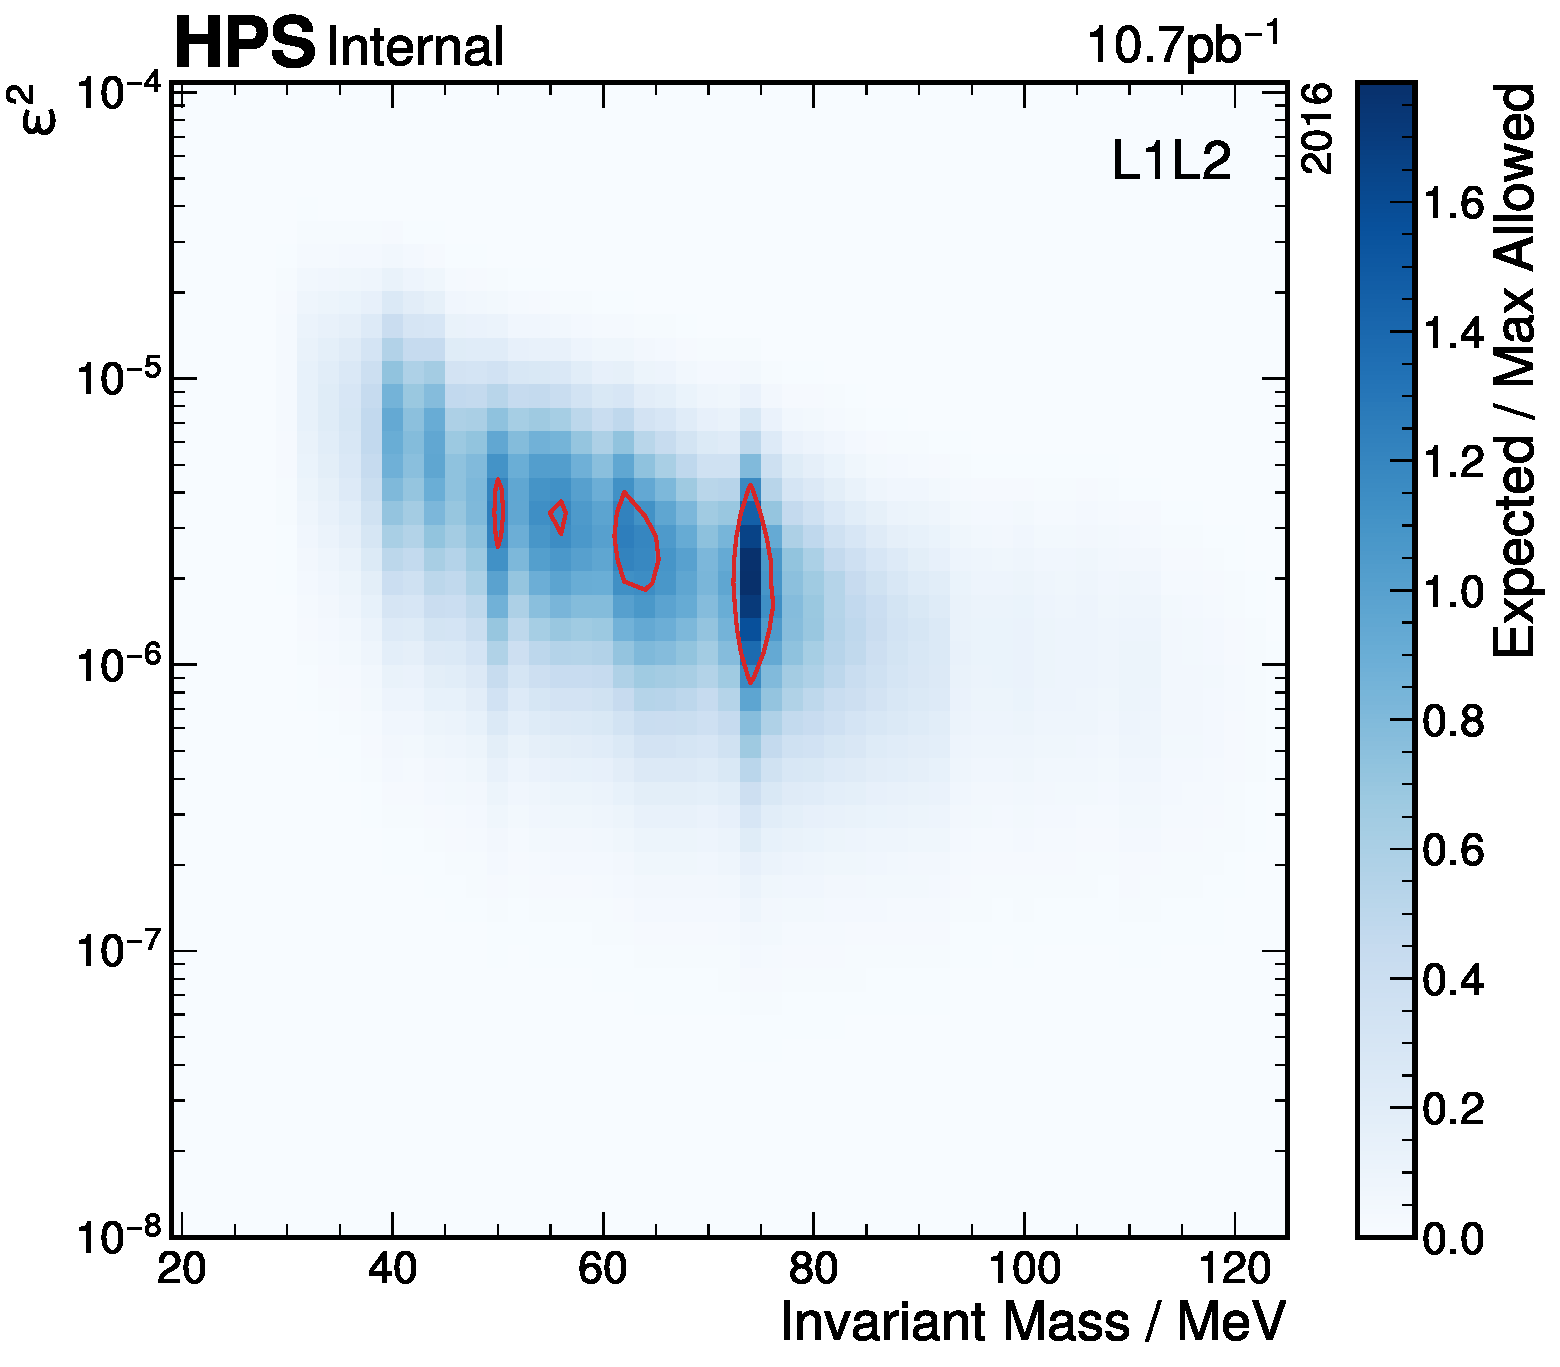
\includegraphics[width=\textwidth]{../figures/hps/analysis/results/exclusion-estimate.pdf}
    \end{column}
    \begin{column}{0.5\textwidth}
      \begin{itemize}
        \item \emph{Naive} (overly-optimistic) estimate
        \item Combination of OIM results with L1L1
          \begin{itemize}
            \item Slightly extends reach in core sensitivity region
          \end{itemize}
      \end{itemize}
      \begin{center}
        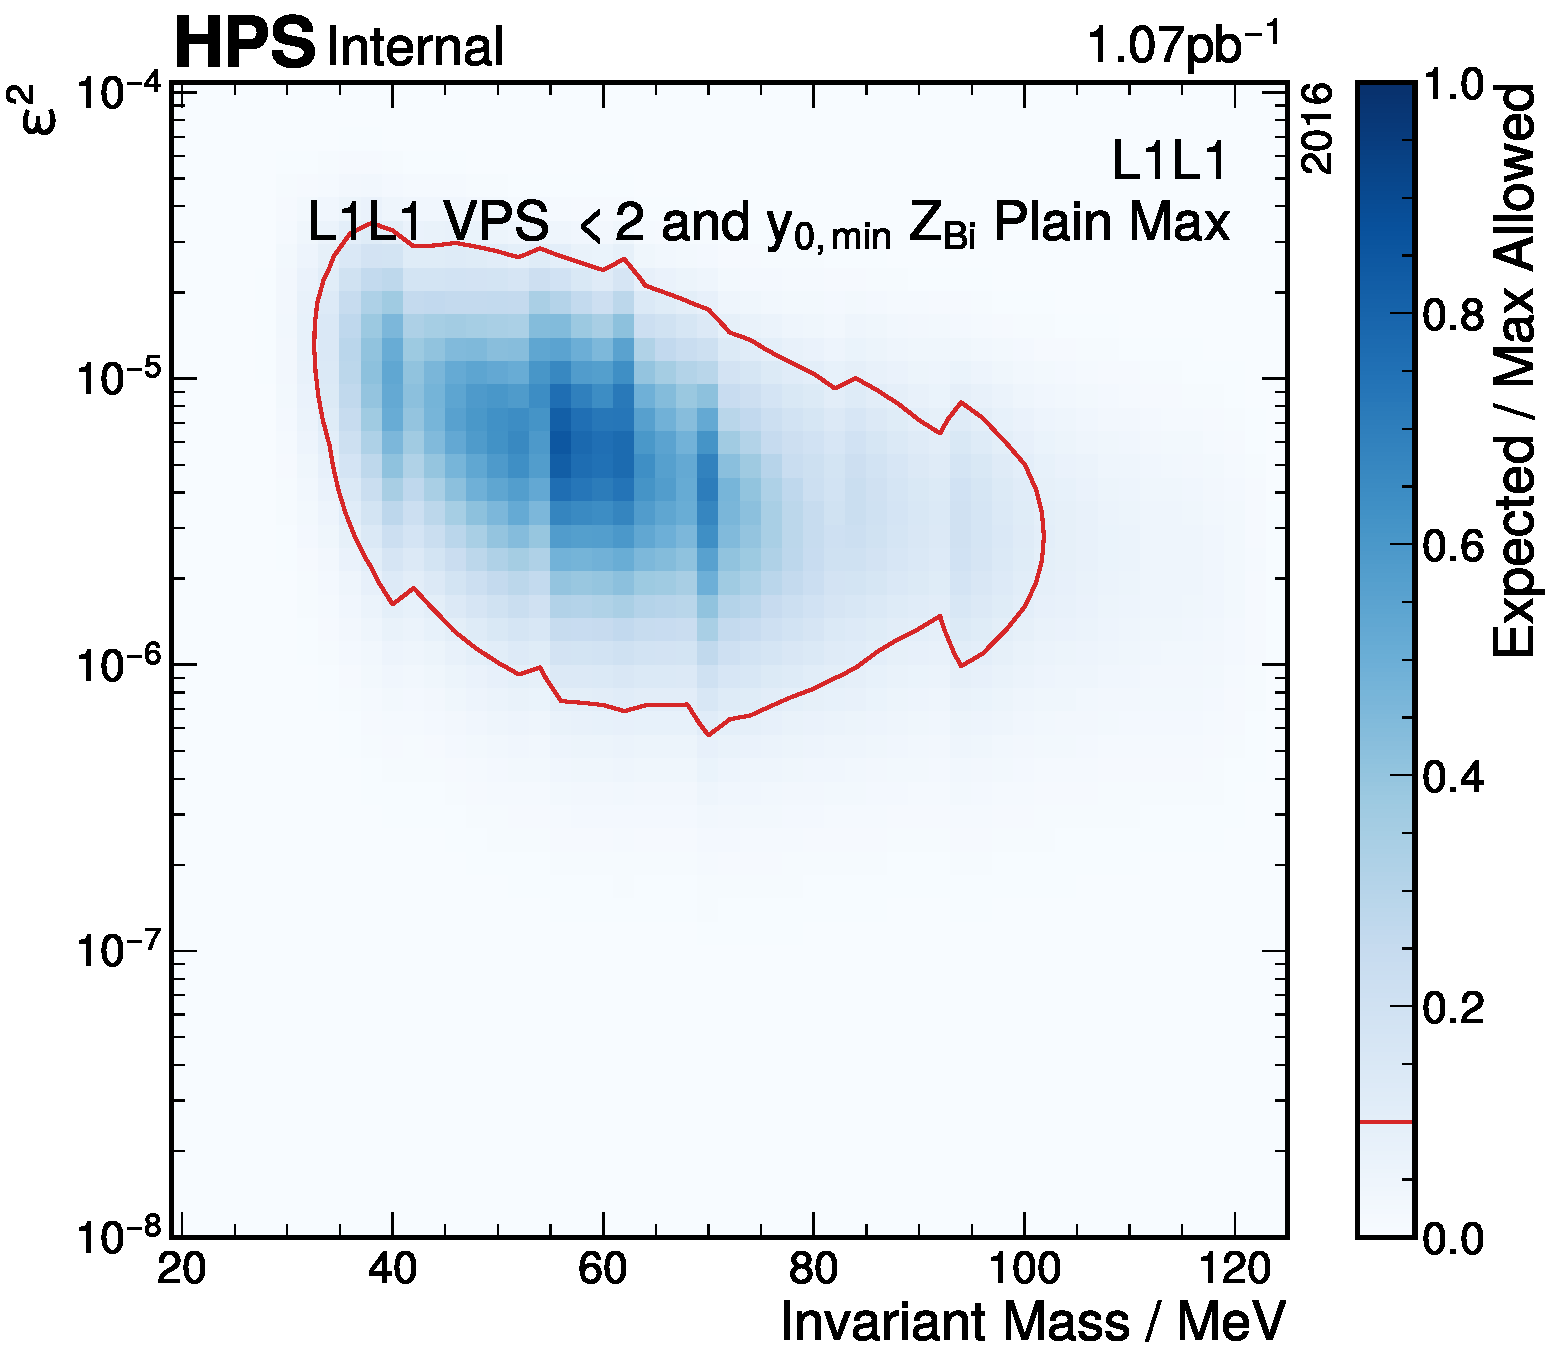
\includegraphics[height=0.4\textheight]{../figures/hps/analysis/results/l1l1-exclusion-estimate.pdf}
      \end{center}
    \end{column}
  \end{columns}
\end{frame}

\note[itemize]{
\item Calculate expected signal using SIMP model and use the \ac{oim}
  to estimate the maximum allowed signal yield
\item Ratio of these quantities gives the sensitivity within 10\%
\item Contour drawn at a value of 0.1 is a naive estimate
\item Combining this result with the L1L1 result solidifies the exclusion
  and lowers the contour in the core mass region
\item Contour Shape roughly made of three lines
  \begin{itemize}
    \item Bottom of triangle determined by data volume (are enough A' produced?)
    \item Top of triangle determined by decay length (does DM decay within HPS acceptance?)
    \item Left side determined by opening angle (smaller mass, more boost, pair more likely to go through central hole of HPS)
  \end{itemize}
}

\ssection{Conclusion}

\begin{frame}{Conclusion}
  Many ways to search for many types of \ac{dm}
  
  \begin{block}{LDMX}
    Missing momentum/energy search still in preparatory stages
  \end{block}

  \begin{block}{HPS}
    Excess highly-displaced events at specific mass searching within
    data for different \ac{dm} models
  \end{block}

  \begin{center}
    \color{UMNSunny}
    Both enable investigation of novel phase space
    in physics' quest to find \ac{dm}
  \end{center}
\end{frame}

\begin{backup}

\begin{frame}{LDMX Midshower Simulation Samples}
  \begin{table}
    \begin{tabular}{|c|c|c|}
    \hline
    Sample & Biasing Factor & Biasing Threshold
    \\ \hline
    Signal & $m_A^{\max(\log_{10}(m_A),2))}/\epsilon^2$ & $0.5E_\text{Beam}$
    \\
    Enriched Nuclear & $200$ & $0.375E_\text{Beam}$
    \\
    Di-Muon & $10^5$ & $0.5E_\text{Beam}$
    \\
    \hline \hline
    Sample & \multicolumn{2}{c|}{Filtering Cuts}
    \\ \hline
    Unbiased  
        & \multicolumn{2}{c|}{$E_{\text{primary}}^{\text{ECal Front}} \geq 0.875E_\text{Beam}$}
    \\
    Signal 
        & \multicolumn{2}{c|}{$E_{\text{primary}}^{\text{ECal Front}} \geq 0.875E_\text{Beam}$ \& $E_{A'}\geq 0.5E_\text{Beam}$}
    \\
    Enriched Nuclear
        & \multicolumn{2}{c|}{$E_{\text{primary}}^{\text{ECal Front}} \geq 0.875E_\text{Beam}$ \& $E_{\text{tot nuc}}\geq 0.625E_\text{Beam}$}
    \\
    Di-Muon
        & \multicolumn{2}{c|}{$E_{\text{primary}}^{\text{ECal Front}} \geq 0.875E_\text{Beam}$ \& $E_{\text{tot}~\mu}\geq 0.5E_\text{Beam}$}
    \\ \hline
\end{tabular}

    \caption{Configuration of the simulation samples used in this analysis. $E_\mathrm{beam}$ is the beam energy being studied ($4$ or $8$ GeV in this work). $m_A$ is the mass of the A' in MeV, $\epsilon$ is the dark brem mixing strength, $E_{\text{primary}}^{\text{ECal Front}}$ is the energy of the primary electron at the front of the ECal, $E_{A'}$ is the energy of the generated A', $E_{\text{tot nuc}}$ is the total energy transferred to nuclear interactions during the event, and $E_{\text{tot}~\mu}$ is the total energy of produced muons.}
  \end{table}
\end{frame}

\begin{frame}{HPS Modified ABCD(EF) Search Method}
  \begin{columns}
    \begin{column}{0.5\textwidth}
      \centering
      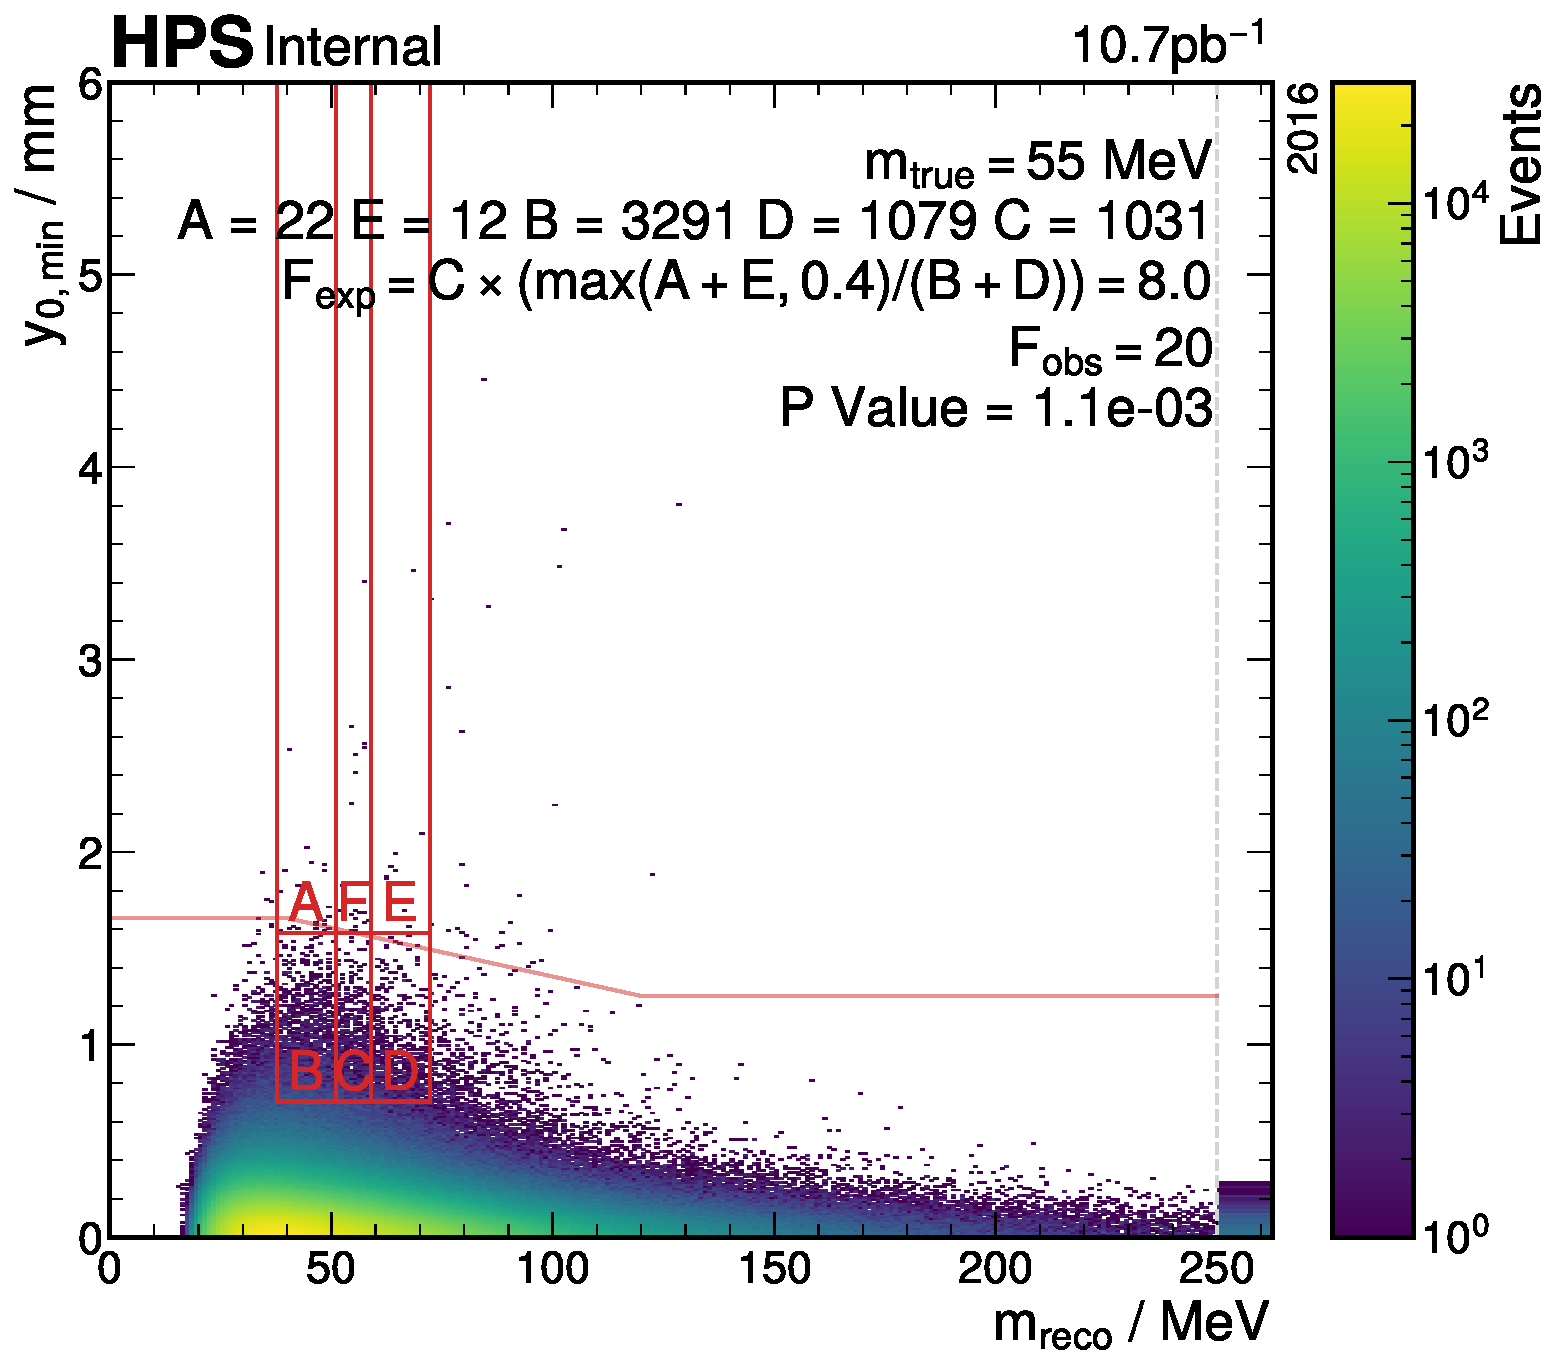
\includegraphics[width=\textwidth]{../figures/hps/analysis/results/search-min-p-val.pdf}
    \end{column}
    \begin{column}{0.5\textwidth}
      \begin{enumerate}
        \item Fill histogram with data
        \item Set mass edges at $1.5\sigma$ and $4.5\sigma$ (values optimized by A Spellmen)
        \item Set upper \minyzero edge at cut value
        \item Lower other \minyzero edge (a.k.a. $y_0$ ``floor'') from the cut value
          until there are at least 1k events in region C
        \item Calculate expected number of events in F
          and compare to observed number of events
        \item Estimate p-value by throwing toy experiments in A+E (Poission), B+D
          and C (Normal) and re-calculating F from these toys
      \end{enumerate}
    \end{column}
  \end{columns}
\end{frame}

\end{backup}

\end{document} 
